% La compilacion se debe hacer con la instruccion de PdfLatex
% para evitar problemas de tamaño de hoja.
% Todos los archivos de figuras deben estar en formato PDF.
% Al momento de imprimir el documento, se debe hacer sin escala de pagina.
\documentclass[letterpaper,12pt]{cicese}
%%%%%%%%%%%%%%%%%%%%%%%%%%%%%%%%%%%%%%%%%%%%%%%%%%%%%%%%%%%%%%%%%%%%%%%%%%%%%%%%%%%%%%%%%%%%%%%%%%%%%%%%%%%%%%%%%%%%%%%%%%%%%%%%%%%%%%%%%%%%%%%%%%%%%%%%%%%%%%%%%%%%%%%%%%%%%%%%%%%%%%%%%%%%%%%%%%%%%%%%%%%%%%%%%%%%%%%%%%%%%%%%%%%%%%%%%%%%%%%%%%%%%%%%%%%%
\usepackage{ marvosym }
\usepackage[letterpaper,left=3cm,right=2cm,top=2cm,bottom=2cm]{geometry}
%%\usepackage[ansinew]{inputenc}   %este paquete es para poner acentos directamente en el codigo de latex. sin barra
%%\usepackage[T1]{fontenc}
%\usepackage[spanish,english]{babel}
%%\usepackage[spanish,mexico,es-lcroman]{babel}
%paquete para insertar hipervinculos en referencias a capitulos, figuras, etc.
\usepackage{helvet}
\renewcommand{\familydefault}{\sfdefault} 
\usepackage[spanish, mexico,es-lcroman]{babel}
\usepackage[utf8x]{inputenc}
\usepackage{mdframed}
\usepackage[acronym]{glossaries}
\makeglossaries
\usepackage[linkcolor=blue]{hyperref}
\usepackage{cicese}
\usepackage{tabularx}
\usepackage{pbox}
\usepackage{makeidx}
\usepackage{eurosym}
\usepackage{amssymb}
\usepackage{amsmath}
\usepackage{gensymb}
\usepackage{graphicx} % figuras
\graphicspath{{figures//}}
\usepackage{natbib} 
\usepackage{emptypage} 
\usepackage{textcomp}
%\usepackage[linesnumbered,ruled,vlined]{algorithm2e}

\setlength{\parskip}{12pt plus 1pt minus 1pt}


% Paquete para pseudocodigo o algoritmos
%\usepackage[lined,boxed,boxruled,linesnumbered,spanish]{algorithm2e}
% Paquete para las graficas
\usepackage{float}
% Paquete para las enumeraciones
\usepackage{enumerate}
% Paquete para pseudocodigo o algoritmos
%este es el que venía:
%\usepackage[lined,boxed,boxruled,linesnumbered,spanish]{algorithm2e}

\usepackage{algorithm}
\usepackage{algorithmic}
\floatname{algorithm}{Algoritmo}
\renewcommand{\listalgorithmname}{Lista de algoritmos}
\renewcommand{\algorithmicrequire}{\textbf{Entrada:}}
\renewcommand{\algorithmicensure}{\textbf{Salida:}}
\renewcommand{\algorithmicend}{\textbf{fin}}
\renewcommand{\algorithmicif}{\textbf{si}}
\renewcommand{\algorithmicthen}{\textbf{entonces}}
\renewcommand{\algorithmicelse}{\textbf{si no}}
\renewcommand{\algorithmicelsif}{\algorithmicelse,\ \algorithmicif}
\renewcommand{\algorithmicendif}{\algorithmicend\ \algorithmicif}
\renewcommand{\algorithmicfor}{\textbf{para}}
\renewcommand{\algorithmicforall}{\textbf{para todo}}
\renewcommand{\algorithmicdo}{\textbf{hacer}}
\renewcommand{\algorithmicendfor}{\algorithmicend\ \algorithmicfor}
\renewcommand{\algorithmicwhile}{\textbf{mientras}}
\renewcommand{\algorithmicendwhile}{\algorithmicend\ \algorithmicwhile}
\renewcommand{\algorithmicloop}{\textbf{repetir}}
\renewcommand{\algorithmicendloop}{\algorithmicend\ \algorithmicloop}
\renewcommand{\algorithmicrepeat}{\textbf{repetir}}
\renewcommand{\algorithmicuntil}{\textbf{hasta que}}
\renewcommand{\algorithmicprint}{\textbf{imprimir}} 
\renewcommand{\algorithmicreturn}{\textbf{regresar}} 
\renewcommand{\algorithmictrue}{\textbf{cierto }} 
\renewcommand{\algorithmicfalse}{\textbf{falso }} 
 % mi archivo de traducción

\usepackage{titlesec}
%\titleformat{\chapter}[display]
%  {\normalfont\huge\bfseries}{\chaptertitlename\ \thechapter}{16pt}{\Huge}
  
\titleformat{\chapter} % command
[hang] % shape
{\normalfont\bfseries\Large} % format
{\chaptertitlename\ \thechapter .} % label
{
16pt
} % sep
{
%    \rule{\textwidth}{1pt}
%    \vspace{1ex}
%    \centering
} % before-code
[
\vspace{-2ex}%
%\rule{\textwidth}{0.3pt}
] % after-code

%\titlespacing{command}{left spacing}{before spacing}{after spacing}[right]
\titlespacing\chapter{0pt}{-40.25pt plus 4pt minus 2pt}{12pt plus 2pt minus 2pt}
\titlespacing\section{0pt}{0pt plus 4pt minus 2pt}{3pt plus 2pt minus 2pt}
\titlespacing\subsection{0pt}{0pt plus 4pt minus 2pt}{3pt plus 2pt minus 2pt}
\titlespacing\subsubsection{0pt}{0pt plus 4pt minus 2pt}{3pt plus 2pt minus 2pt}

  	
% Paquete para estilizar los captions de tablas e imagenes
\usepackage[font=footnotesize,format=plain,labelfont=bf,up,textfont=bf,md,up,justification=justified]{caption}
\captionsetup{labelfont=bf}

% Para cambiar el color de fondo de una celda en una tabla
\usepackage[table]{xcolor}	
% Para rotar una tabla
\usepackage{rotating}
%\usepackage{subfig}
\usepackage{subfigure} % subfiguras
% Asignar espacio personalizado
\usepackage{setspace}
% Para hacer tablas de multiples páginas
\usepackage{longtable}
% Para utilizar multiples renglones en tablas
\usepackage{multirow}
\usepackage{booktabs}


%%%%%%%%%%%%%%%%%%%%%%%%%%%%%%%%%%%%
%para agregar teoremas, etc

\newtheorem{theorem}{Teorema}[chapter]
\newenvironment{proof}{\noindent{\bf Demostraci\'on.}}{\hfill$\blacksquare$} 
\newtheorem{lemma}{Lema}[chapter]
\newtheorem{teo}{Teorema}[chapter]
\newtheorem{obs}{Observaci\'on}[chapter]
\setcounter{MaxMatrixCols}{10}

% Macros for Scientific Word 4.0 documents saved with the LaTeX filter.
% Copyright (C) 2002 Mackichan Software, Inc.

\typeout{TCILATEX Macros for Scientific Word 5.0 <13 Feb 2003>.}
\typeout{NOTICE:  This macro file is NOT proprietary and may be 
freely copied and distributed.}
%
\makeatletter

%%%%%%%%%%%%%%%%%%%%%
% pdfTeX related.
\ifx\pdfoutput\relax\let\pdfoutput=\undefined\fi
\newcount\msipdfoutput
\ifx\pdfoutput\undefined
\else
 \ifcase\pdfoutput
 \else 
    \msipdfoutput=1
    \ifx\paperwidth\undefined
    \else
      \ifdim\paperheight=0pt\relax
      \else
        \pdfpageheight\paperheight
      \fi
      \ifdim\paperwidth=0pt\relax
      \else
        \pdfpagewidth\paperwidth
      \fi
    \fi
  \fi  
\fi

%%%%%%%%%%%%%%%%%%%%%
% FMTeXButton
% This is used for putting TeXButtons in the 
% frontmatter of a document. Add a line like
% \QTagDef{FMTeXButton}{101}{} to the filter 
% section of the cst being used. Also add a
% new section containing:
%     [f_101]
%     ALIAS=FMTexButton
%     TAG_TYPE=FIELD
%     TAG_LEADIN=TeX Button:
%
% It also works to put \defs in the preamble after 
% the \input tcilatex
\def\FMTeXButton#1{#1}
%
%%%%%%%%%%%%%%%%%%%%%%
% macros for time
\newcount\@hour\newcount\@minute\chardef\@x10\chardef\@xv60
\def\tcitime{
\def\@time{%
  \@minute\time\@hour\@minute\divide\@hour\@xv
  \ifnum\@hour<\@x 0\fi\the\@hour:%
  \multiply\@hour\@xv\advance\@minute-\@hour
  \ifnum\@minute<\@x 0\fi\the\@minute
  }}%

%%%%%%%%%%%%%%%%%%%%%%
% macro for hyperref and msihyperref
%\@ifundefined{hyperref}{\def\hyperref#1#2#3#4{#2\ref{#4}#3}}{}

\def\x@hyperref#1#2#3{%
   % Turn off various catcodes before reading parameter 4
   \catcode`\~ = 12
   \catcode`\$ = 12
   \catcode`\_ = 12
   \catcode`\# = 12
   \catcode`\& = 12
   \y@hyperref{#1}{#2}{#3}%
}

\def\y@hyperref#1#2#3#4{%
   #2\ref{#4}#3
   \catcode`\~ = 13
   \catcode`\$ = 3
   \catcode`\_ = 8
   \catcode`\# = 6
   \catcode`\& = 4
}

\@ifundefined{hyperref}{\let\hyperref\x@hyperref}{}
\@ifundefined{msihyperref}{\let\msihyperref\x@hyperref}{}




% macro for external program call
\@ifundefined{qExtProgCall}{\def\qExtProgCall#1#2#3#4#5#6{\relax}}{}
%%%%%%%%%%%%%%%%%%%%%%
%
% macros for graphics
%
\def\FILENAME#1{#1}%
%
\def\QCTOpt[#1]#2{%
  \def\QCTOptB{#1}
  \def\QCTOptA{#2}
}
\def\QCTNOpt#1{%
  \def\QCTOptA{#1}
  \let\QCTOptB\empty
}
\def\Qct{%
  \@ifnextchar[{%
    \QCTOpt}{\QCTNOpt}
}
\def\QCBOpt[#1]#2{%
  \def\QCBOptB{#1}%
  \def\QCBOptA{#2}%
}
\def\QCBNOpt#1{%
  \def\QCBOptA{#1}%
  \let\QCBOptB\empty
}
\def\Qcb{%
  \@ifnextchar[{%
    \QCBOpt}{\QCBNOpt}%
}
\def\PrepCapArgs{%
  \ifx\QCBOptA\empty
    \ifx\QCTOptA\empty
      {}%
    \else
      \ifx\QCTOptB\empty
        {\QCTOptA}%
      \else
        [\QCTOptB]{\QCTOptA}%
      \fi
    \fi
  \else
    \ifx\QCBOptA\empty
      {}%
    \else
      \ifx\QCBOptB\empty
        {\QCBOptA}%
      \else
        [\QCBOptB]{\QCBOptA}%
      \fi
    \fi
  \fi
}
\newcount\GRAPHICSTYPE
%\GRAPHICSTYPE 0 is for TurboTeX
%\GRAPHICSTYPE 1 is for DVIWindo (PostScript)
%%%(removed)%\GRAPHICSTYPE 2 is for psfig (PostScript)
\GRAPHICSTYPE=\z@
\def\GRAPHICSPS#1{%
 \ifcase\GRAPHICSTYPE%\GRAPHICSTYPE=0
   \special{ps: #1}%
 \or%\GRAPHICSTYPE=1
   \special{language "PS", include "#1"}%
%%%\or%\GRAPHICSTYPE=2
%%%  #1%
 \fi
}%
%
\def\GRAPHICSHP#1{\special{include #1}}%
%
% \graffile{ body }                                  %#1
%          { contentswidth (scalar)  }               %#2
%          { contentsheight (scalar) }               %#3
%          { vertical shift when in-line (scalar) }  %#4

\def\graffile#1#2#3#4{%
%%% \ifnum\GRAPHICSTYPE=\tw@
%%%  %Following if using psfig
%%%  \@ifundefined{psfig}{\input psfig.tex}{}%
%%%  \psfig{file=#1, height=#3, width=#2}%
%%% \else
  %Following for all others
  % JCS - added BOXTHEFRAME, see below
    \bgroup
	   \@inlabelfalse
       \leavevmode
       \@ifundefined{bbl@deactivate}{\def~{\string~}}{\activesoff}%
        \raise -#4 \BOXTHEFRAME{%
           \hbox to #2{\raise #3\hbox to #2{\null #1\hfil}}}%
    \egroup
}%
%
% A box for drafts
\def\draftbox#1#2#3#4{%
 \leavevmode\raise -#4 \hbox{%
  \frame{\rlap{\protect\tiny #1}\hbox to #2%
   {\vrule height#3 width\z@ depth\z@\hfil}%
  }%
 }%
}%
%
\newcount\@msidraft
\@msidraft=\z@
\let\nographics=\@msidraft
\newif\ifwasdraft
\wasdraftfalse

%  \GRAPHIC{ body }                                  %#1
%          { draft name }                            %#2
%          { contentswidth (scalar)  }               %#3
%          { contentsheight (scalar) }               %#4
%          { vertical shift when in-line (scalar) }  %#5
\def\GRAPHIC#1#2#3#4#5{%
   \ifnum\@msidraft=\@ne\draftbox{#2}{#3}{#4}{#5}%
   \else\graffile{#1}{#3}{#4}{#5}%
   \fi
}
%
\def\addtoLaTeXparams#1{%
    \edef\LaTeXparams{\LaTeXparams #1}}%
%
% JCS -  added a switch BoxFrame that can 
% be set by including X in the frame params.
% If set a box is drawn around the frame.

\newif\ifBoxFrame \BoxFramefalse
\newif\ifOverFrame \OverFramefalse
\newif\ifUnderFrame \UnderFramefalse

\def\BOXTHEFRAME#1{%
   \hbox{%
      \ifBoxFrame
         \frame{#1}%
      \else
         {#1}%
      \fi
   }%
}


\def\doFRAMEparams#1{\BoxFramefalse\OverFramefalse\UnderFramefalse\readFRAMEparams#1\end}%
\def\readFRAMEparams#1{%
 \ifx#1\end%
  \let\next=\relax
  \else
  \ifx#1i\dispkind=\z@\fi
  \ifx#1d\dispkind=\@ne\fi
  \ifx#1f\dispkind=\tw@\fi
  \ifx#1t\addtoLaTeXparams{t}\fi
  \ifx#1b\addtoLaTeXparams{b}\fi
  \ifx#1p\addtoLaTeXparams{p}\fi
  \ifx#1h\addtoLaTeXparams{h}\fi
  \ifx#1X\BoxFrametrue\fi
  \ifx#1O\OverFrametrue\fi
  \ifx#1U\UnderFrametrue\fi
  \ifx#1w
    \ifnum\@msidraft=1\wasdrafttrue\else\wasdraftfalse\fi
    \@msidraft=\@ne
  \fi
  \let\next=\readFRAMEparams
  \fi
 \next
 }%
%
%Macro for In-line graphics object
%   \IFRAME{ contentswidth (scalar)  }               %#1
%          { contentsheight (scalar) }               %#2
%          { vertical shift when in-line (scalar) }  %#3
%          { draft name }                            %#4
%          { body }                                  %#5
%          { caption}                                %#6


\def\IFRAME#1#2#3#4#5#6{%
      \bgroup
      \let\QCTOptA\empty
      \let\QCTOptB\empty
      \let\QCBOptA\empty
      \let\QCBOptB\empty
      #6%
      \parindent=0pt
      \leftskip=0pt
      \rightskip=0pt
      \setbox0=\hbox{\QCBOptA}%
      \@tempdima=#1\relax
      \ifOverFrame
          % Do this later
          \typeout{This is not implemented yet}%
          \show\HELP
      \else
         \ifdim\wd0>\@tempdima
            \advance\@tempdima by \@tempdima
            \ifdim\wd0 >\@tempdima
               \setbox1 =\vbox{%
                  \unskip\hbox to \@tempdima{\hfill\GRAPHIC{#5}{#4}{#1}{#2}{#3}\hfill}%
                  \unskip\hbox to \@tempdima{\parbox[b]{\@tempdima}{\QCBOptA}}%
               }%
               \wd1=\@tempdima
            \else
               \textwidth=\wd0
               \setbox1 =\vbox{%
                 \noindent\hbox to \wd0{\hfill\GRAPHIC{#5}{#4}{#1}{#2}{#3}\hfill}\\%
                 \noindent\hbox{\QCBOptA}%
               }%
               \wd1=\wd0
            \fi
         \else
            \ifdim\wd0>0pt
              \hsize=\@tempdima
              \setbox1=\vbox{%
                \unskip\GRAPHIC{#5}{#4}{#1}{#2}{0pt}%
                \break
                \unskip\hbox to \@tempdima{\hfill \QCBOptA\hfill}%
              }%
              \wd1=\@tempdima
           \else
              \hsize=\@tempdima
              \setbox1=\vbox{%
                \unskip\GRAPHIC{#5}{#4}{#1}{#2}{0pt}%
              }%
              \wd1=\@tempdima
           \fi
         \fi
         \@tempdimb=\ht1
         %\advance\@tempdimb by \dp1
         \advance\@tempdimb by -#2
         \advance\@tempdimb by #3
         \leavevmode
         \raise -\@tempdimb \hbox{\box1}%
      \fi
      \egroup%
}%
%
%Macro for Display graphics object
%   \DFRAME{ contentswidth (scalar)  }               %#1
%          { contentsheight (scalar) }               %#2
%          { draft label }                           %#3
%          { name }                                  %#4
%          { caption}                                %#5
\def\DFRAME#1#2#3#4#5{%
  \vspace\topsep
  \hfil\break
  \bgroup
     \leftskip\@flushglue
	 \rightskip\@flushglue
	 \parindent\z@
	 \parfillskip\z@skip
     \let\QCTOptA\empty
     \let\QCTOptB\empty
     \let\QCBOptA\empty
     \let\QCBOptB\empty
	 \vbox\bgroup
        \ifOverFrame 
           #5\QCTOptA\par
        \fi
        \GRAPHIC{#4}{#3}{#1}{#2}{\z@}%
        \ifUnderFrame 
           \break#5\QCBOptA
        \fi
	 \egroup
  \egroup
  \vspace\topsep
  \break
}%
%
%Macro for Floating graphic object
%   \FFRAME{ framedata f|i tbph x F|T }              %#1
%          { contentswidth (scalar)  }               %#2
%          { contentsheight (scalar) }               %#3
%          { caption }                               %#4
%          { label }                                 %#5
%          { draft name }                            %#6
%          { body }                                  %#7
\def\FFRAME#1#2#3#4#5#6#7{%
 %If float.sty loaded and float option is 'h', change to 'H'  (gp) 1998/09/05
  \@ifundefined{floatstyle}
    {%floatstyle undefined (and float.sty not present), no change
     \begin{figure}[#1]%
    }
    {%floatstyle DEFINED
	 \ifx#1h%Only the h parameter, change to H
      \begin{figure}[H]%
	 \else
      \begin{figure}[#1]%
	 \fi
	}
  \let\QCTOptA\empty
  \let\QCTOptB\empty
  \let\QCBOptA\empty
  \let\QCBOptB\empty
  \ifOverFrame
    #4
    \ifx\QCTOptA\empty
    \else
      \ifx\QCTOptB\empty
        \caption{\QCTOptA}%
      \else
        \caption[\QCTOptB]{\QCTOptA}%
      \fi
    \fi
    \ifUnderFrame\else
      \label{#5}%
    \fi
  \else
    \UnderFrametrue%
  \fi
  \begin{center}\GRAPHIC{#7}{#6}{#2}{#3}{\z@}\end{center}%
  \ifUnderFrame
    #4
    \ifx\QCBOptA\empty
      \caption{}%
    \else
      \ifx\QCBOptB\empty
        \caption{\QCBOptA}%
      \else
        \caption[\QCBOptB]{\QCBOptA}%
      \fi
    \fi
    \label{#5}%
  \fi
  \end{figure}%
 }%
%
%
%    \FRAME{ framedata f|i tbph x F|T }              %#1
%          { contentswidth (scalar)  }               %#2
%          { contentsheight (scalar) }               %#3
%          { vertical shift when in-line (scalar) }  %#4
%          { caption }                               %#5
%          { label }                                 %#6
%          { name }                                  %#7
%          { body }                                  %#8
%
%    framedata is a string which can contain the following
%    characters: idftbphxFT
%    Their meaning is as follows:
%             i, d or f : in-line, display, or floating
%             t,b,p,h   : LaTeX floating placement options
%             x         : fit contents box to contents
%             F or T    : Figure or Table. 
%                         Later this can expand
%                         to a more general float class.
%
%
\newcount\dispkind%

\def\makeactives{
  \catcode`\"=\active
  \catcode`\;=\active
  \catcode`\:=\active
  \catcode`\'=\active
  \catcode`\~=\active
}
\bgroup
   \makeactives
   \gdef\activesoff{%
      \def"{\string"}%
      \def;{\string;}%
      \def:{\string:}%
      \def'{\string'}%
      \def~{\string~}%
      %\bbl@deactivate{"}%
      %\bbl@deactivate{;}%
      %\bbl@deactivate{:}%
      %\bbl@deactivate{'}%
    }
\egroup

\def\FRAME#1#2#3#4#5#6#7#8{%
 \bgroup
 \ifnum\@msidraft=\@ne
   \wasdrafttrue
 \else
   \wasdraftfalse%
 \fi
 \def\LaTeXparams{}%
 \dispkind=\z@
 \def\LaTeXparams{}%
 \doFRAMEparams{#1}%
 \ifnum\dispkind=\z@\IFRAME{#2}{#3}{#4}{#7}{#8}{#5}\else
  \ifnum\dispkind=\@ne\DFRAME{#2}{#3}{#7}{#8}{#5}\else
   \ifnum\dispkind=\tw@
    \edef\@tempa{\noexpand\FFRAME{\LaTeXparams}}%
    \@tempa{#2}{#3}{#5}{#6}{#7}{#8}%
    \fi
   \fi
  \fi
  \ifwasdraft\@msidraft=1\else\@msidraft=0\fi{}%
  \egroup
 }%
%
% This macro added to let SW gobble a parameter that
% should not be passed on and expanded. 

\def\TEXUX#1{"texux"}

%
% Macros for text attributes:
%
\def\BF#1{{\bf {#1}}}%
\def\NEG#1{\leavevmode\hbox{\rlap{\thinspace/}{$#1$}}}%
%
%%%%%%%%%%%%%%%%%%%%%%%%%%%%%%%%%%%%%%%%%%%%%%%%%%%%%%%%%%%%%%%%%%%%%%%%
%
%
% macros for user - defined functions
\def\limfunc#1{\mathop{\rm #1}}%
\def\func#1{\mathop{\rm #1}\nolimits}%
% macro for unit names
\def\unit#1{\mathord{\thinspace\rm #1}}%

%
% miscellaneous 
\long\def\QQQ#1#2{%
     \long\expandafter\def\csname#1\endcsname{#2}}%
\@ifundefined{QTP}{\def\QTP#1{}}{}
\@ifundefined{QEXCLUDE}{\def\QEXCLUDE#1{}}{}
\@ifundefined{Qlb}{\def\Qlb#1{#1}}{}
\@ifundefined{Qlt}{\def\Qlt#1{#1}}{}
\def\QWE{}%
\long\def\QQA#1#2{}%
\def\QTR#1#2{{\csname#1\endcsname {#2}}}%
\long\def\TeXButton#1#2{#2}%
\long\def\QSubDoc#1#2{#2}%
\def\EXPAND#1[#2]#3{}%
\def\NOEXPAND#1[#2]#3{}%
\def\PROTECTED{}%
\def\LaTeXparent#1{}%
\def\ChildStyles#1{}%
\def\ChildDefaults#1{}%
\def\QTagDef#1#2#3{}%

% Constructs added with Scientific Notebook
\@ifundefined{correctchoice}{\def\correctchoice{\relax}}{}
\@ifundefined{HTML}{\def\HTML#1{\relax}}{}
\@ifundefined{TCIIcon}{\def\TCIIcon#1#2#3#4{\relax}}{}
\if@compatibility
  \typeout{Not defining UNICODE  U or CustomNote commands for LaTeX 2.09.}
\else
  \providecommand{\UNICODE}[2][]{\protect\rule{.1in}{.1in}}
  \providecommand{\U}[1]{\protect\rule{.1in}{.1in}}
  \providecommand{\CustomNote}[3][]{\marginpar{#3}}
\fi

\@ifundefined{lambdabar}{
      \def\lambdabar{\errmessage{You have used the lambdabar symbol. 
                      This is available for typesetting only in RevTeX styles.}}
   }{}

%
% Macros for style editor docs
\@ifundefined{StyleEditBeginDoc}{\def\StyleEditBeginDoc{\relax}}{}
%
% Macros for footnotes
\def\QQfnmark#1{\footnotemark}
\def\QQfntext#1#2{\addtocounter{footnote}{#1}\footnotetext{#2}}
%
% Macros for indexing.
%
\@ifundefined{TCIMAKEINDEX}{}{\makeindex}%
%
% Attempts to avoid problems with other styles
\@ifundefined{abstract}{%
 \def\abstract{%
  \if@twocolumn
   \section*{Abstract (Not appropriate in this style!)}%
   \else \small 
   \begin{center}{\bf Abstract\vspace{-.5em}\vspace{\z@}}\end{center}%
   \quotation 
   \fi
  }%
 }{%
 }%
\@ifundefined{endabstract}{\def\endabstract
  {\if@twocolumn\else\endquotation\fi}}{}%
\@ifundefined{maketitle}{\def\maketitle#1{}}{}%
\@ifundefined{affiliation}{\def\affiliation#1{}}{}%
\@ifundefined{proof}{\def\proof{\noindent{\bfseries Proof. }}}{}%
\@ifundefined{endproof}{\def\endproof{\mbox{\ \rule{.1in}{.1in}}}}{}%
\@ifundefined{newfield}{\def\newfield#1#2{}}{}%
\@ifundefined{chapter}{\def\chapter#1{\par(Chapter head:)#1\par }%
 \newcount\c@chapter}{}%
\@ifundefined{part}{\def\part#1{\par(Part head:)#1\par }}{}%
\@ifundefined{section}{\def\section#1{\par(Section head:)#1\par }}{}%
\@ifundefined{subsection}{\def\subsection#1%
 {\par(Subsection head:)#1\par }}{}%
\@ifundefined{subsubsection}{\def\subsubsection#1%
 {\par(Subsubsection head:)#1\par }}{}%
\@ifundefined{paragraph}{\def\paragraph#1%
 {\par(Subsubsubsection head:)#1\par }}{}%
\@ifundefined{subparagraph}{\def\subparagraph#1%
 {\par(Subsubsubsubsection head:)#1\par }}{}%
%%%%%%%%%%%%%%%%%%%%%%%%%%%%%%%%%%%%%%%%%%%%%%%%%%%%%%%%%%%%%%%%%%%%%%%%
% These symbols are not recognized by LaTeX
\@ifundefined{therefore}{\def\therefore{}}{}%
\@ifundefined{backepsilon}{\def\backepsilon{}}{}%
\@ifundefined{yen}{\def\yen{\hbox{\rm\rlap=Y}}}{}%
\@ifundefined{registered}{%
   \def\registered{\relax\ifmmode{}\r@gistered
                    \else$\m@th\r@gistered$\fi}%
 \def\r@gistered{^{\ooalign
  {\hfil\raise.07ex\hbox{$\scriptstyle\rm\text{R}$}\hfil\crcr
  \mathhexbox20D}}}}{}%
\@ifundefined{Eth}{\def\Eth{}}{}%
\@ifundefined{eth}{\def\eth{}}{}%
\@ifundefined{Thorn}{\def\Thorn{}}{}%
\@ifundefined{thorn}{\def\thorn{}}{}%
% A macro to allow any symbol that requires math to appear in text
\def\TEXTsymbol#1{\mbox{$#1$}}%
\@ifundefined{degree}{\def\degree{{}^{\circ}}}{}%
%
% macros for T3TeX files
\newdimen\theight
\@ifundefined{Column}{\def\Column{%
 \vadjust{\setbox\z@=\hbox{\scriptsize\quad\quad tcol}%
  \theight=\ht\z@\advance\theight by \dp\z@\advance\theight by \lineskip
  \kern -\theight \vbox to \theight{%
   \rightline{\rlap{\box\z@}}%
   \vss
   }%
  }%
 }}{}%
%
\@ifundefined{qed}{\def\qed{%
 \ifhmode\unskip\nobreak\fi\ifmmode\ifinner\else\hskip5\p@\fi\fi
 \hbox{\hskip5\p@\vrule width4\p@ height6\p@ depth1.5\p@\hskip\p@}%
 }}{}%
%
\@ifundefined{cents}{\def\cents{\hbox{\rm\rlap c/}}}{}%
\@ifundefined{tciLaplace}{\def\tciLaplace{\ensuremath{\mathcal{L}}}}{}%
\@ifundefined{tciFourier}{\def\tciFourier{\ensuremath{\mathcal{F}}}}{}%
\@ifundefined{textcurrency}{\def\textcurrency{\hbox{\rm\rlap xo}}}{}%
\@ifundefined{texteuro}{\def\texteuro{\hbox{\rm\rlap C=}}}{}%
\@ifundefined{euro}{\def\euro{\hbox{\rm\rlap C=}}}{}%
\@ifundefined{textfranc}{\def\textfranc{\hbox{\rm\rlap-F}}}{}%
\@ifundefined{textlira}{\def\textlira{\hbox{\rm\rlap L=}}}{}%
\@ifundefined{textpeseta}{\def\textpeseta{\hbox{\rm P\negthinspace s}}}{}%
%
\@ifundefined{miss}{\def\miss{\hbox{\vrule height2\p@ width 2\p@ depth\z@}}}{}%
%
\@ifundefined{vvert}{\def\vvert{\Vert}}{}%  %always translated to \left| or \right|
%
\@ifundefined{tcol}{\def\tcol#1{{\baselineskip=6\p@ \vcenter{#1}} \Column}}{}%
%
\@ifundefined{dB}{\def\dB{\hbox{{}}}}{}%        %dummy entry in column 
\@ifundefined{mB}{\def\mB#1{\hbox{$#1$}}}{}%   %column entry
\@ifundefined{nB}{\def\nB#1{\hbox{#1}}}{}%     %column entry (not math)
%
\@ifundefined{note}{\def\note{$^{\dag}}}{}%
%
\def\newfmtname{LaTeX2e}
% No longer load latexsym.  This is now handled by SWP, which uses amsfonts if necessary
%
\ifx\fmtname\newfmtname
  \DeclareOldFontCommand{\rm}{\normalfont\rmfamily}{\mathrm}
  \DeclareOldFontCommand{\sf}{\normalfont\sffamily}{\mathsf}
  \DeclareOldFontCommand{\tt}{\normalfont\ttfamily}{\mathtt}
  \DeclareOldFontCommand{\bf}{\normalfont\bfseries}{\mathbf}
  \DeclareOldFontCommand{\it}{\normalfont\itshape}{\mathit}
  \DeclareOldFontCommand{\sl}{\normalfont\slshape}{\@nomath\sl}
  \DeclareOldFontCommand{\sc}{\normalfont\scshape}{\@nomath\sc}
\fi

%
% Greek bold macros
% Redefine all of the math symbols 
% which might be bolded	 - there are 
% probably others to add to this list

\def\alpha{{\Greekmath 010B}}%
\def\beta{{\Greekmath 010C}}%
\def\gamma{{\Greekmath 010D}}%
\def\delta{{\Greekmath 010E}}%
\def\epsilon{{\Greekmath 010F}}%
\def\zeta{{\Greekmath 0110}}%
\def\eta{{\Greekmath 0111}}%
\def\theta{{\Greekmath 0112}}%
\def\iota{{\Greekmath 0113}}%
\def\kappa{{\Greekmath 0114}}%
\def\lambda{{\Greekmath 0115}}%
\def\mu{{\Greekmath 0116}}%
\def\nu{{\Greekmath 0117}}%
\def\xi{{\Greekmath 0118}}%
\def\pi{{\Greekmath 0119}}%
\def\rho{{\Greekmath 011A}}%
\def\sigma{{\Greekmath 011B}}%
\def\tau{{\Greekmath 011C}}%
\def\upsilon{{\Greekmath 011D}}%
\def\phi{{\Greekmath 011E}}%
\def\chi{{\Greekmath 011F}}%
\def\psi{{\Greekmath 0120}}%
\def\omega{{\Greekmath 0121}}%
\def\varepsilon{{\Greekmath 0122}}%
\def\vartheta{{\Greekmath 0123}}%
\def\varpi{{\Greekmath 0124}}%
\def\varrho{{\Greekmath 0125}}%
\def\varsigma{{\Greekmath 0126}}%
\def\varphi{{\Greekmath 0127}}%

\def\nabla{{\Greekmath 0272}}
\def\FindBoldGroup{%
   {\setbox0=\hbox{$\mathbf{x\global\edef\theboldgroup{\the\mathgroup}}$}}%
}

\def\Greekmath#1#2#3#4{%
    \if@compatibility
        \ifnum\mathgroup=\symbold
           \mathchoice{\mbox{\boldmath$\displaystyle\mathchar"#1#2#3#4$}}%
                      {\mbox{\boldmath$\textstyle\mathchar"#1#2#3#4$}}%
                      {\mbox{\boldmath$\scriptstyle\mathchar"#1#2#3#4$}}%
                      {\mbox{\boldmath$\scriptscriptstyle\mathchar"#1#2#3#4$}}%
        \else
           \mathchar"#1#2#3#4% 
        \fi 
    \else 
        \FindBoldGroup
        \ifnum\mathgroup=\theboldgroup % For 2e
           \mathchoice{\mbox{\boldmath$\displaystyle\mathchar"#1#2#3#4$}}%
                      {\mbox{\boldmath$\textstyle\mathchar"#1#2#3#4$}}%
                      {\mbox{\boldmath$\scriptstyle\mathchar"#1#2#3#4$}}%
                      {\mbox{\boldmath$\scriptscriptstyle\mathchar"#1#2#3#4$}}%
        \else
           \mathchar"#1#2#3#4% 
        \fi     	    
	  \fi}

\newif\ifGreekBold  \GreekBoldfalse
\let\SAVEPBF=\pbf
\def\pbf{\GreekBoldtrue\SAVEPBF}%
%

\@ifundefined{theorem}{\newtheorem{theorem}{Theorem}}{}
\@ifundefined{lemma}{\newtheorem{lemma}[theorem]{Lemma}}{}
\@ifundefined{corollary}{\newtheorem{corollary}[theorem]{Corollary}}{}
\@ifundefined{conjecture}{\newtheorem{conjecture}[theorem]{Conjecture}}{}
\@ifundefined{proposition}{\newtheorem{proposition}[theorem]{Proposition}}{}
\@ifundefined{axiom}{\newtheorem{axiom}{Axiom}}{}
\@ifundefined{remark}{\newtheorem{remark}{Remark}}{}
\@ifundefined{example}{\newtheorem{example}{Example}}{}
\@ifundefined{exercise}{\newtheorem{exercise}{Exercise}}{}
\@ifundefined{definition}{\newtheorem{definition}{Definition}}{}


\@ifundefined{mathletters}{%
  %\def\theequation{\arabic{equation}}
  \newcounter{equationnumber}  
  \def\mathletters{%
     \addtocounter{equation}{1}
     \edef\@currentlabel{\theequation}%
     \setcounter{equationnumber}{\c@equation}
     \setcounter{equation}{0}%
     \edef\theequation{\@currentlabel\noexpand\alph{equation}}%
  }
  \def\endmathletters{%
     \setcounter{equation}{\value{equationnumber}}%
  }
}{}

%Logos
\@ifundefined{BibTeX}{%
    \def\BibTeX{{\rm B\kern-.05em{\sc i\kern-.025em b}\kern-.08em
                 T\kern-.1667em\lower.7ex\hbox{E}\kern-.125emX}}}{}%
\@ifundefined{AmS}%
    {\def\AmS{{\protect\usefont{OMS}{cmsy}{m}{n}%
                A\kern-.1667em\lower.5ex\hbox{M}\kern-.125emS}}}{}%
\@ifundefined{AmSTeX}{\def\AmSTeX{\protect\AmS-\protect\TeX\@}}{}%
%

% This macro is a fix to eqnarray
\def\@@eqncr{\let\@tempa\relax
    \ifcase\@eqcnt \def\@tempa{& & &}\or \def\@tempa{& &}%
      \else \def\@tempa{&}\fi
     \@tempa
     \if@eqnsw
        \iftag@
           \@taggnum
        \else
           \@eqnnum\stepcounter{equation}%
        \fi
     \fi
     \global\tag@false
     \global\@eqnswtrue
     \global\@eqcnt\z@\cr}


\def\TCItag{\@ifnextchar*{\@TCItagstar}{\@TCItag}}
\def\@TCItag#1{%
    \global\tag@true
    \global\def\@taggnum{(#1)}}
\def\@TCItagstar*#1{%
    \global\tag@true
    \global\def\@taggnum{#1}}
%
%%%%%%%%%%%%%%%%%%%%%%%%%%%%%%%%%%%%%%%%%%%%%%%%%%%%%%%%%%%%%%%%%%%%%
%
\def\QATOP#1#2{{#1 \atop #2}}%
\def\QTATOP#1#2{{\textstyle {#1 \atop #2}}}%
\def\QDATOP#1#2{{\displaystyle {#1 \atop #2}}}%
\def\QABOVE#1#2#3{{#2 \above#1 #3}}%
\def\QTABOVE#1#2#3{{\textstyle {#2 \above#1 #3}}}%
\def\QDABOVE#1#2#3{{\displaystyle {#2 \above#1 #3}}}%
\def\QOVERD#1#2#3#4{{#3 \overwithdelims#1#2 #4}}%
\def\QTOVERD#1#2#3#4{{\textstyle {#3 \overwithdelims#1#2 #4}}}%
\def\QDOVERD#1#2#3#4{{\displaystyle {#3 \overwithdelims#1#2 #4}}}%
\def\QATOPD#1#2#3#4{{#3 \atopwithdelims#1#2 #4}}%
\def\QTATOPD#1#2#3#4{{\textstyle {#3 \atopwithdelims#1#2 #4}}}%
\def\QDATOPD#1#2#3#4{{\displaystyle {#3 \atopwithdelims#1#2 #4}}}%
\def\QABOVED#1#2#3#4#5{{#4 \abovewithdelims#1#2#3 #5}}%
\def\QTABOVED#1#2#3#4#5{{\textstyle 
   {#4 \abovewithdelims#1#2#3 #5}}}%
\def\QDABOVED#1#2#3#4#5{{\displaystyle 
   {#4 \abovewithdelims#1#2#3 #5}}}%
%
% Macros for text size operators:
%
\def\tint{\mathop{\textstyle \int}}%
\def\tiint{\mathop{\textstyle \iint }}%
\def\tiiint{\mathop{\textstyle \iiint }}%
\def\tiiiint{\mathop{\textstyle \iiiint }}%
\def\tidotsint{\mathop{\textstyle \idotsint }}%
\def\toint{\mathop{\textstyle \oint}}%
\def\tsum{\mathop{\textstyle \sum }}%
\def\tprod{\mathop{\textstyle \prod }}%
\def\tbigcap{\mathop{\textstyle \bigcap }}%
\def\tbigwedge{\mathop{\textstyle \bigwedge }}%
\def\tbigoplus{\mathop{\textstyle \bigoplus }}%
\def\tbigodot{\mathop{\textstyle \bigodot }}%
\def\tbigsqcup{\mathop{\textstyle \bigsqcup }}%
\def\tcoprod{\mathop{\textstyle \coprod }}%
\def\tbigcup{\mathop{\textstyle \bigcup }}%
\def\tbigvee{\mathop{\textstyle \bigvee }}%
\def\tbigotimes{\mathop{\textstyle \bigotimes }}%
\def\tbiguplus{\mathop{\textstyle \biguplus }}%
%
%
%Macros for display size operators:
%
\def\dint{\mathop{\displaystyle \int}}%
\def\diint{\mathop{\displaystyle \iint}}%
\def\diiint{\mathop{\displaystyle \iiint}}%
\def\diiiint{\mathop{\displaystyle \iiiint }}%
\def\didotsint{\mathop{\displaystyle \idotsint }}%
\def\doint{\mathop{\displaystyle \oint}}%
\def\dsum{\mathop{\displaystyle \sum }}%
\def\dprod{\mathop{\displaystyle \prod }}%
\def\dbigcap{\mathop{\displaystyle \bigcap }}%
\def\dbigwedge{\mathop{\displaystyle \bigwedge }}%
\def\dbigoplus{\mathop{\displaystyle \bigoplus }}%
\def\dbigodot{\mathop{\displaystyle \bigodot }}%
\def\dbigsqcup{\mathop{\displaystyle \bigsqcup }}%
\def\dcoprod{\mathop{\displaystyle \coprod }}%
\def\dbigcup{\mathop{\displaystyle \bigcup }}%
\def\dbigvee{\mathop{\displaystyle \bigvee }}%
\def\dbigotimes{\mathop{\displaystyle \bigotimes }}%
\def\dbiguplus{\mathop{\displaystyle \biguplus }}%

\if@compatibility\else
  % Always load amsmath in LaTeX2e mode
  \RequirePackage{amsmath}
\fi

\def\ExitTCILatex{\makeatother\endinput}

\bgroup
\ifx\ds@amstex\relax
   \message{amstex already loaded}\aftergroup\ExitTCILatex
\else
   \@ifpackageloaded{amsmath}%
      {\if@compatibility\message{amsmath already loaded}\fi\aftergroup\ExitTCILatex}
      {}
   \@ifpackageloaded{amstex}%
      {\if@compatibility\message{amstex already loaded}\fi\aftergroup\ExitTCILatex}
      {}
   \@ifpackageloaded{amsgen}%
      {\if@compatibility\message{amsgen already loaded}\fi\aftergroup\ExitTCILatex}
      {}
\fi
\egroup

%Exit if any of the AMS macros are already loaded.
%This is always the case for LaTeX2e mode.


%%%%%%%%%%%%%%%%%%%%%%%%%%%%%%%%%%%%%%%%%%%%%%%%%%%%%%%%%%%%%%%%%%%%%%%%%%
% NOTE: The rest of this file is read only if in LaTeX 2.09 compatibility
% mode. This section is used to define AMS-like constructs in the
% event they have not been defined.
%%%%%%%%%%%%%%%%%%%%%%%%%%%%%%%%%%%%%%%%%%%%%%%%%%%%%%%%%%%%%%%%%%%%%%%%%%
\typeout{TCILATEX defining AMS-like constructs in LaTeX 2.09 COMPATIBILITY MODE}
%%%%%%%%%%%%%%%%%%%%%%%%%%%%%%%%%%%%%%%%%%%%%%%%%%%%%%%%%%%%%%%%%%%%%%%%
%  Macros to define some AMS LaTeX constructs when 
%  AMS LaTeX has not been loaded
% 
% These macros are copied from the AMS-TeX package for doing
% multiple integrals.
%
\let\DOTSI\relax
\def\RIfM@{\relax\ifmmode}%
\def\FN@{\futurelet\next}%
\newcount\intno@
\def\iint{\DOTSI\intno@\tw@\FN@\ints@}%
\def\iiint{\DOTSI\intno@\thr@@\FN@\ints@}%
\def\iiiint{\DOTSI\intno@4 \FN@\ints@}%
\def\idotsint{\DOTSI\intno@\z@\FN@\ints@}%
\def\ints@{\findlimits@\ints@@}%
\newif\iflimtoken@
\newif\iflimits@
\def\findlimits@{\limtoken@true\ifx\next\limits\limits@true
 \else\ifx\next\nolimits\limits@false\else
 \limtoken@false\ifx\ilimits@\nolimits\limits@false\else
 \ifinner\limits@false\else\limits@true\fi\fi\fi\fi}%
\def\multint@{\int\ifnum\intno@=\z@\intdots@                          %1
 \else\intkern@\fi                                                    %2
 \ifnum\intno@>\tw@\int\intkern@\fi                                   %3
 \ifnum\intno@>\thr@@\int\intkern@\fi                                 %4
 \int}%                                                               %5
\def\multintlimits@{\intop\ifnum\intno@=\z@\intdots@\else\intkern@\fi
 \ifnum\intno@>\tw@\intop\intkern@\fi
 \ifnum\intno@>\thr@@\intop\intkern@\fi\intop}%
\def\intic@{%
    \mathchoice{\hskip.5em}{\hskip.4em}{\hskip.4em}{\hskip.4em}}%
\def\negintic@{\mathchoice
 {\hskip-.5em}{\hskip-.4em}{\hskip-.4em}{\hskip-.4em}}%
\def\ints@@{\iflimtoken@                                              %1
 \def\ints@@@{\iflimits@\negintic@
   \mathop{\intic@\multintlimits@}\limits                             %2
  \else\multint@\nolimits\fi                                          %3
  \eat@}%                                                             %4
 \else                                                                %5
 \def\ints@@@{\iflimits@\negintic@
  \mathop{\intic@\multintlimits@}\limits\else
  \multint@\nolimits\fi}\fi\ints@@@}%
\def\intkern@{\mathchoice{\!\!\!}{\!\!}{\!\!}{\!\!}}%
\def\plaincdots@{\mathinner{\cdotp\cdotp\cdotp}}%
\def\intdots@{\mathchoice{\plaincdots@}%
 {{\cdotp}\mkern1.5mu{\cdotp}\mkern1.5mu{\cdotp}}%
 {{\cdotp}\mkern1mu{\cdotp}\mkern1mu{\cdotp}}%
 {{\cdotp}\mkern1mu{\cdotp}\mkern1mu{\cdotp}}}%
%
%
%  These macros are for doing the AMS \text{} construct
%
\def\RIfM@{\relax\protect\ifmmode}
\def\text{\RIfM@\expandafter\text@\else\expandafter\mbox\fi}
\let\nfss@text\text
\def\text@#1{\mathchoice
   {\textdef@\displaystyle\f@size{#1}}%
   {\textdef@\textstyle\tf@size{\firstchoice@false #1}}%
   {\textdef@\textstyle\sf@size{\firstchoice@false #1}}%
   {\textdef@\textstyle \ssf@size{\firstchoice@false #1}}%
   \glb@settings}

\def\textdef@#1#2#3{\hbox{{%
                    \everymath{#1}%
                    \let\f@size#2\selectfont
                    #3}}}
\newif\iffirstchoice@
\firstchoice@true
%
%These are the AMS constructs for multiline limits.
%
\def\Let@{\relax\iffalse{\fi\let\\=\cr\iffalse}\fi}%
\def\vspace@{\def\vspace##1{\crcr\noalign{\vskip##1\relax}}}%
\def\multilimits@{\bgroup\vspace@\Let@
 \baselineskip\fontdimen10 \scriptfont\tw@
 \advance\baselineskip\fontdimen12 \scriptfont\tw@
 \lineskip\thr@@\fontdimen8 \scriptfont\thr@@
 \lineskiplimit\lineskip
 \vbox\bgroup\ialign\bgroup\hfil$\m@th\scriptstyle{##}$\hfil\crcr}%
\def\Sb{_\multilimits@}%
\def\endSb{\crcr\egroup\egroup\egroup}%
\def\Sp{^\multilimits@}%
\let\endSp\endSb
%
%
%These are AMS constructs for horizontal arrows
%
\newdimen\ex@
\ex@.2326ex
\def\rightarrowfill@#1{$#1\m@th\mathord-\mkern-6mu\cleaders
 \hbox{$#1\mkern-2mu\mathord-\mkern-2mu$}\hfill
 \mkern-6mu\mathord\rightarrow$}%
\def\leftarrowfill@#1{$#1\m@th\mathord\leftarrow\mkern-6mu\cleaders
 \hbox{$#1\mkern-2mu\mathord-\mkern-2mu$}\hfill\mkern-6mu\mathord-$}%
\def\leftrightarrowfill@#1{$#1\m@th\mathord\leftarrow
\mkern-6mu\cleaders
 \hbox{$#1\mkern-2mu\mathord-\mkern-2mu$}\hfill
 \mkern-6mu\mathord\rightarrow$}%
\def\overrightarrow{\mathpalette\overrightarrow@}%
\def\overrightarrow@#1#2{\vbox{\ialign{##\crcr\rightarrowfill@#1\crcr
 \noalign{\kern-\ex@\nointerlineskip}$\m@th\hfil#1#2\hfil$\crcr}}}%
\let\overarrow\overrightarrow
\def\overleftarrow{\mathpalette\overleftarrow@}%
\def\overleftarrow@#1#2{\vbox{\ialign{##\crcr\leftarrowfill@#1\crcr
 \noalign{\kern-\ex@\nointerlineskip}$\m@th\hfil#1#2\hfil$\crcr}}}%
\def\overleftrightarrow{\mathpalette\overleftrightarrow@}%
\def\overleftrightarrow@#1#2{\vbox{\ialign{##\crcr
   \leftrightarrowfill@#1\crcr
 \noalign{\kern-\ex@\nointerlineskip}$\m@th\hfil#1#2\hfil$\crcr}}}%
\def\underrightarrow{\mathpalette\underrightarrow@}%
\def\underrightarrow@#1#2{\vtop{\ialign{##\crcr$\m@th\hfil#1#2\hfil
  $\crcr\noalign{\nointerlineskip}\rightarrowfill@#1\crcr}}}%
\let\underarrow\underrightarrow
\def\underleftarrow{\mathpalette\underleftarrow@}%
\def\underleftarrow@#1#2{\vtop{\ialign{##\crcr$\m@th\hfil#1#2\hfil
  $\crcr\noalign{\nointerlineskip}\leftarrowfill@#1\crcr}}}%
\def\underleftrightarrow{\mathpalette\underleftrightarrow@}%
\def\underleftrightarrow@#1#2{\vtop{\ialign{##\crcr$\m@th
  \hfil#1#2\hfil$\crcr
 \noalign{\nointerlineskip}\leftrightarrowfill@#1\crcr}}}%
%%%%%%%%%%%%%%%%%%%%%

\def\qopnamewl@#1{\mathop{\operator@font#1}\nlimits@}
\let\nlimits@\displaylimits
\def\setboxz@h{\setbox\z@\hbox}


\def\varlim@#1#2{\mathop{\vtop{\ialign{##\crcr
 \hfil$#1\m@th\operator@font lim$\hfil\crcr
 \noalign{\nointerlineskip}#2#1\crcr
 \noalign{\nointerlineskip\kern-\ex@}\crcr}}}}

 \def\rightarrowfill@#1{\m@th\setboxz@h{$#1-$}\ht\z@\z@
  $#1\copy\z@\mkern-6mu\cleaders
  \hbox{$#1\mkern-2mu\box\z@\mkern-2mu$}\hfill
  \mkern-6mu\mathord\rightarrow$}
\def\leftarrowfill@#1{\m@th\setboxz@h{$#1-$}\ht\z@\z@
  $#1\mathord\leftarrow\mkern-6mu\cleaders
  \hbox{$#1\mkern-2mu\copy\z@\mkern-2mu$}\hfill
  \mkern-6mu\box\z@$}


\def\projlim{\qopnamewl@{proj\,lim}}
\def\injlim{\qopnamewl@{inj\,lim}}
\def\varinjlim{\mathpalette\varlim@\rightarrowfill@}
\def\varprojlim{\mathpalette\varlim@\leftarrowfill@}
\def\varliminf{\mathpalette\varliminf@{}}
\def\varliminf@#1{\mathop{\underline{\vrule\@depth.2\ex@\@width\z@
   \hbox{$#1\m@th\operator@font lim$}}}}
\def\varlimsup{\mathpalette\varlimsup@{}}
\def\varlimsup@#1{\mathop{\overline
  {\hbox{$#1\m@th\operator@font lim$}}}}

%
%Companion to stackrel
\def\stackunder#1#2{\mathrel{\mathop{#2}\limits_{#1}}}%
%
%
% These are AMS environments that will be defined to
% be verbatims if amstex has not actually been 
% loaded
%
%
\begingroup \catcode `|=0 \catcode `[= 1
\catcode`]=2 \catcode `\{=12 \catcode `\}=12
\catcode`\\=12 
|gdef|@alignverbatim#1\end{align}[#1|end[align]]
|gdef|@salignverbatim#1\end{align*}[#1|end[align*]]

|gdef|@alignatverbatim#1\end{alignat}[#1|end[alignat]]
|gdef|@salignatverbatim#1\end{alignat*}[#1|end[alignat*]]

|gdef|@xalignatverbatim#1\end{xalignat}[#1|end[xalignat]]
|gdef|@sxalignatverbatim#1\end{xalignat*}[#1|end[xalignat*]]

|gdef|@gatherverbatim#1\end{gather}[#1|end[gather]]
|gdef|@sgatherverbatim#1\end{gather*}[#1|end[gather*]]

|gdef|@gatherverbatim#1\end{gather}[#1|end[gather]]
|gdef|@sgatherverbatim#1\end{gather*}[#1|end[gather*]]


|gdef|@multilineverbatim#1\end{multiline}[#1|end[multiline]]
|gdef|@smultilineverbatim#1\end{multiline*}[#1|end[multiline*]]

|gdef|@arraxverbatim#1\end{arrax}[#1|end[arrax]]
|gdef|@sarraxverbatim#1\end{arrax*}[#1|end[arrax*]]

|gdef|@tabulaxverbatim#1\end{tabulax}[#1|end[tabulax]]
|gdef|@stabulaxverbatim#1\end{tabulax*}[#1|end[tabulax*]]


|endgroup
  

  
\def\align{\@verbatim \frenchspacing\@vobeyspaces \@alignverbatim
You are using the "align" environment in a style in which it is not defined.}
\let\endalign=\endtrivlist
 
\@namedef{align*}{\@verbatim\@salignverbatim
You are using the "align*" environment in a style in which it is not defined.}
\expandafter\let\csname endalign*\endcsname =\endtrivlist




\def\alignat{\@verbatim \frenchspacing\@vobeyspaces \@alignatverbatim
You are using the "alignat" environment in a style in which it is not defined.}
\let\endalignat=\endtrivlist
 
\@namedef{alignat*}{\@verbatim\@salignatverbatim
You are using the "alignat*" environment in a style in which it is not defined.}
\expandafter\let\csname endalignat*\endcsname =\endtrivlist




\def\xalignat{\@verbatim \frenchspacing\@vobeyspaces \@xalignatverbatim
You are using the "xalignat" environment in a style in which it is not defined.}
\let\endxalignat=\endtrivlist
 
\@namedef{xalignat*}{\@verbatim\@sxalignatverbatim
You are using the "xalignat*" environment in a style in which it is not defined.}
\expandafter\let\csname endxalignat*\endcsname =\endtrivlist




\def\gather{\@verbatim \frenchspacing\@vobeyspaces \@gatherverbatim
You are using the "gather" environment in a style in which it is not defined.}
\let\endgather=\endtrivlist
 
\@namedef{gather*}{\@verbatim\@sgatherverbatim
You are using the "gather*" environment in a style in which it is not defined.}
\expandafter\let\csname endgather*\endcsname =\endtrivlist


\def\multiline{\@verbatim \frenchspacing\@vobeyspaces \@multilineverbatim
You are using the "multiline" environment in a style in which it is not defined.}
\let\endmultiline=\endtrivlist
 
\@namedef{multiline*}{\@verbatim\@smultilineverbatim
You are using the "multiline*" environment in a style in which it is not defined.}
\expandafter\let\csname endmultiline*\endcsname =\endtrivlist


\def\arrax{\@verbatim \frenchspacing\@vobeyspaces \@arraxverbatim
You are using a type of "array" construct that is only allowed in AmS-LaTeX.}
\let\endarrax=\endtrivlist

\def\tabulax{\@verbatim \frenchspacing\@vobeyspaces \@tabulaxverbatim
You are using a type of "tabular" construct that is only allowed in AmS-LaTeX.}
\let\endtabulax=\endtrivlist

 
\@namedef{arrax*}{\@verbatim\@sarraxverbatim
You are using a type of "array*" construct that is only allowed in AmS-LaTeX.}
\expandafter\let\csname endarrax*\endcsname =\endtrivlist

\@namedef{tabulax*}{\@verbatim\@stabulaxverbatim
You are using a type of "tabular*" construct that is only allowed in AmS-LaTeX.}
\expandafter\let\csname endtabulax*\endcsname =\endtrivlist

% macro to simulate ams tag construct


% This macro is a fix to the equation environment
 \def\endequation{%
     \ifmmode\ifinner % FLEQN hack
      \iftag@
        \addtocounter{equation}{-1} % undo the increment made in the begin part
        $\hfil
           \displaywidth\linewidth\@taggnum\egroup \endtrivlist
        \global\tag@false
        \global\@ignoretrue   
      \else
        $\hfil
           \displaywidth\linewidth\@eqnnum\egroup \endtrivlist
        \global\tag@false
        \global\@ignoretrue 
      \fi
     \else   
      \iftag@
        \addtocounter{equation}{-1} % undo the increment made in the begin part
        \eqno \hbox{\@taggnum}
        \global\tag@false%
        $$\global\@ignoretrue
      \else
        \eqno \hbox{\@eqnnum}% $$ BRACE MATCHING HACK
        $$\global\@ignoretrue
      \fi
     \fi\fi
 } 

 \newif\iftag@ \tag@false
 
 \def\TCItag{\@ifnextchar*{\@TCItagstar}{\@TCItag}}
 \def\@TCItag#1{%
     \global\tag@true
     \global\def\@taggnum{(#1)}}
 \def\@TCItagstar*#1{%
     \global\tag@true
     \global\def\@taggnum{#1}}

  \@ifundefined{tag}{
     \def\tag{\@ifnextchar*{\@tagstar}{\@tag}}
     \def\@tag#1{%
         \global\tag@true
         \global\def\@taggnum{(#1)}}
     \def\@tagstar*#1{%
         \global\tag@true
         \global\def\@taggnum{#1}}
  }{}

\def\tfrac#1#2{{\textstyle {#1 \over #2}}}%
\def\dfrac#1#2{{\displaystyle {#1 \over #2}}}%
\def\binom#1#2{{#1 \choose #2}}%
\def\tbinom#1#2{{\textstyle {#1 \choose #2}}}%
\def\dbinom#1#2{{\displaystyle {#1 \choose #2}}}%

% Do not add anything to the end of this file.  
% The last section of the file is loaded only if 
% amstex has not been.
\makeatother
\endinput

\setcounter{secnumdepth}{3}
\setcounter{tocdepth}{3}
\begin{document}

% Escribe tu nombre, tal y como aparece en los registros
% de Posgrado. De ser necesario, separa con \- las sílabas
% de tu nombre
\autor{Dari\'en Alberto Miranda Boj\'orquez}

% Escribe el título de tu tesis (Si el titulo es mayor de 2 renglones es necesario
% cambiar el valor de espacio vertical para que conserve las dimensiones del margen.
% La modificacion se hace en el archivo cicese.sty en la seccion de la portada que
% ya esta indicado las dimensiones que debe tener para 3 renglones.)
\titulo{Detecci\'on de ansiedad en cuidadores de personas con demencia por medio de c\'omputo vestible}

% Para el resumen, escribe aqui el título en inglés
\tituloIN{Anxiety detection on caregivers of people with dementia trough wearable computing}

% Aquí va el nombre de tu programa de posgrado
\posgrado{Ciencias de la Computación}
\posgradoUP{CIENCIAS DE LA COMPUTACIÓN}
%con orientaci\'on en \uppercase\expandafter{C\'omputo Biomolecular}
% Aquí va el nombre de orientacion para el que aplique (sino comentarlo)
%\orientacion{}

% Escribe aquí el nombre del posgrado en inglés
\posgradoIN{Computer Science}
%with orientation in \uppercase\expandafter{Biomolecular Computing}
% Escribe aquí el nombre de orientacion para el que aplique (sino comentarlo)
\orientacionIN{}

% El nombre del grado en inglés
\gradoIN{Master in Computer Science}

% Este comando especifica si la tesis es de maestria (usa \mc) o de
% doctorado (usa \dc)
\mc

% Fecha (mes y año) de la defensa de tesis, en español y en ingles
\fechaexamen{Septiembre, 2015}\fechaexamenIN{September, 2015}

% Fecha (dia, mes y año) de la defensa de tesis para la hoja de firmas
\fechaexamencompleta{Septiembre, 2015}

% Año de la defensa //Este valor a aparecerá en la parte inferior de la primer página de la tesis
\anioDefensa{2015}

% Nombre de tu director de tesis, si tienes codirector repite el comando
\director{Dr. Jes\'us Favela Vara}
%\director{Dr. Asesor 2}

% Nombres de los sinodales, en el orden que aparecerán en la
% página de firmas
%%NO UTILIZAR ABREVIATURAS
\sinodal{Dra. Tentori Espinosa M\'onica Elizabeth}
\sinodal{Dr. Chavez Gonz\'alez Edgar Leonel}
\sinodal{Dra. Herzka Llona Sharon Zinah}
\sinodal{Dra. Beatriz Cordero Esquivel}
%\sinodal{Dr. 4}
%\sinodal{Dr. 5}
%\sinodal{Dr. 6}

% Nombre del Director de Estudios de Posgrado
\dirposgrado{Dr. Jesús Favela Vara}
% Nombre del Coordinador del Programa de Posgrado
\cpp{Dra. Ana Isabel Martínez García}

% Escribe aqui el nombre del archivo .tex que contiene el texto del
% resumen en español. Omite escribir la extensión .tex
\resumenES{Resumen}

% Palabras clave del resumen en español
\palabrasclave{Detecci\'on de ansiedad, Cuidadores de personas con demencia, C\'omputo vestible}

% Escribe aqui el nombre del archivo .tex que contiene el texto del
% resumen en inglés. Omite escribir la extensión .tex
\resumenIN{Abstract}

% Palabras clave del resumen en inglés
\keywords{Anxiety detection, Caregivers of people with dementia, Wearable computing}

% Nombre del archivo .tex con el texto de la dedicatoria, omite
% la extensión .tex
\dedicatoria{Dedicatoria}

% Nombre del archivo .tex con el texto de los agradecimientos, omite
% la extensión .tex
\agradecimientos{Agradecimientos}

% Este comando crea todas las páginas preliminares de la tesis
\preliminares

{\normalsize
%TCIMACRO{\QSubDoc{Include Capitulo01}{
\chapter{Amazing title}\label{capit:cap1}
\vspace{-2.0325ex}%
\noindent
\rule{\textwidth}{0.5pt}
\vspace{-5.5ex}% 
\newcommand{\pushline}{\Indp}% Indent puede ir o no :p


Allasdasdsa asdasd sads the stuff goes here ... Acéntos y eñes kshdfhfg jhgdfjhg dsjgsd gdf 

This text is normal size, but
\large
all of this text is pretty big!
Except for a couple
{\Large really} big
{\LARGE obnoxiously} large
{\Huge words}.
You can get back down to size with some
{\normalsize normal text}.
If you're feeling
{\small small}, you can get really
{\tiny tiny}, but you can also imitate other sizes like
{\footnotesize footnotes} and
{\scriptsize subscripts and superscripts}







\newpage
%%=====================================================
} }%
%BeginExpansion

\chapter{Amazing title}\label{capit:cap1}
\vspace{-2.0325ex}%
\noindent
\rule{\textwidth}{0.5pt}
\vspace{-5.5ex}% 
\newcommand{\pushline}{\Indp}% Indent puede ir o no :p


Allasdasdsa asdasd sads the stuff goes here ... Acéntos y eñes kshdfhfg jhgdfjhg dsjgsd gdf 

This text is normal size, but
\large
all of this text is pretty big!
Except for a couple
{\Large really} big
{\LARGE obnoxiously} large
{\Huge words}.
You can get back down to size with some
{\normalsize normal text}.
If you're feeling
{\small small}, you can get really
{\tiny tiny}, but you can also imitate other sizes like
{\footnotesize footnotes} and
{\scriptsize subscripts and superscripts}







\newpage
%%=====================================================

%EndExpansion
\newpage }

{\normalsize
%TCIMACRO{\QSubDoc{Include Capitulo02}{\chapter{Fundamentos te\'oricos}\label{capit:cap2}
\vspace{-2.0325ex}%
\noindent
\rule{\textwidth}{0.5pt}
\vspace{-5.5ex}% 
\newcommand{\pushline}{\Indp}% Indent puede ir o no :p

\section{Introducci\'on}\label{secc:introduccion}
La ansiedad es un fen\'omeno con el que nuestra sociedad se encuentra \'intimamente relacionada. Todos la sentimos multiples veces a lo largo de nuestras vidas, al dar un discurso en p\'ublico, al ser entrevistado para un nuevo trabajo o durante un examen. Es parte de lo que nos mantiene alertas y listos para enfrentar las situaciones de d\'ia a d\'ia. Sin embargo, solemos no darle la importancia que significa para las personas que sufren de elevados niveles de ansiedad y de los beneficios que la tecnolog\'ia puede brindarles. En este cap\'itulo, se define la ansiedad, la manera en que se origina, como afecta a los cuidadores y como podemos medirla.



\section{Qu\'e es la Ansiedad?}\label{secc:ansiedad}

La ansiedad es una emoci\'on caracterizada por sensaciones de tensi\'on, pensamientos de preocupaci\'on y cambios f\'isicos como incremento en la presi\'on arterial \citep{psychologyapa}, aumento de la sudoraci\'on y palpitaciones, entre otras respuestas fisiol\'ogicas. Estas manifestaciones se dan en determinados lapsos de tiempos durante la vida del individuo. Durante estos lapsos, se dice que el sujeto se encuentra en un estado mental de ansiedad [ref].

Este estado mental es \'util para los humanos, debido a que la ansiedad es una reacci\'on normal del cuerpo para lograr objetivos, o lograr sobrevivir ante a una amenaza. Sin embargo, cuando la persona experimenta un nivel de ansiedad el cual es tan alto que no le permite manejar su vida normal, se dice que la persona tiene un desorden de ansiedad\citep{repetto2013}. 

\subsection{Ansiedad y estr\'es}\label{secc:anxietyandstress}
Si bien, en ocasiones el estr\'es y la ansiedad son conceptos que se usan de manera intercambiable, existen diferencias entre ambos. El estr\'es es definido como el desvalance entre la carga mental dada y la percepci\'on de las habilidades que el individuo tiene para lidiar dicha carga[ref]. Este desvalance puede hacer que la ansiedad aumente, mientras que la ansiedad puede a su vez generar estr\'es. La relaci\'on entre el estr\'es y la ansiedad es la ansiedad es la se\~nal psicofisiol\'ogica de que la respuesta al estr\'es ha sido iniciada \citep{PMID2235645}.


\subsection{``State Anxiety'' y ``Trait Anxiety''}\label{secc:anxieystatevstrait}
Existen dos clasificaciones de ansiedad reconocidas por la \textit{American Psychological Association} \citep{psychologyapa} , ``State Anxiety'' y ``Trait Anxiety'' las cuales se mencionan a continuaci\'on.

\begin{itemize}
	\item{\textbf{State Anxiety:}} Es una manifestaci\'on de ansiedad a cerca de un evento \textbf{presente} bien definido. Normalmente la persona se encuentra conciente de la fuente de su ansiead. 
	\item{\textbf{Trait Anxiety:}} Es una manifestaci\'on a largo plazo de la ansiedad, en la que el individuo puede entrar al estado de ansiedad sin saber la raz\'on concreta. Las personas con personalidades t\'imidas tienden a sufrir mas de este tipo de ansiedad. [ref]

\end{itemize}

A pesar de que los efectos negativos en la calidad de vida de las personas que sufren de ``Trait Anxiety'' son mas fuertes, este trabajo est\'a enfocado en ``State Anxiety'' debido a que es mas f\'acil de cuantificar y medir por medio de sensores.

\section{Demencia}\label{secc:dementia}
La demencia es un s\'indrome del declive de las habilidades cognitivas. Los s\'intomas comunes son: problemas de memoria, dificultades para realizar tareas familiares, mal juicio, deterioro del lenguaje hablado y cambios de humor\citep{Aziz}. Afecta alrededor de el 4\% de las personas mayores de 65 a\~nos y al 40\% de las personas mayores de 90. La demencia suele manifestarse en sindromes como el de Alzheimer. Las personas con demencia necesitan de una persona que cuide de ellos, normalmente durante el resto de su vida. Usualmente necesitan ayuda en las actividades de la vida diaria (Activities of Daily Life), siendo esto una carga para los cuidadores.

\section{Cuidadores}\label{secc:caregivers}
Uno de los sectores de poblaci\'on vulnerables, son los cuidadores de personas con demencia. Se encuentra documentado que los cuidadores, al llevar una carga f\'isica, cognitiva y emocional derivada de su labor les genera padecimientos como ansiedad, estr\'es, y hasta la muerte\citep{Chen2013}. Debido a que los cuidadores no necesariamente son personas con una formaci\'on profesional, estos efectos pueden verse aumentados. Por lo general, los cuidadores que son familiares del paciente son a\'un m\'as afectados ya que necesitan administrar el tiempo de trabajo, familia, actividades sociales y la actividad misma del cuidado del paciente.
			%Cuales son las situaciones ( escenarios ) en los que los CUIDADORES presentan ansiedad?

\subsection{C\'omo se genera la ansiedad en los cuidadores?}\label{secc:caregiverburden}

\begin{figure}[h]
	\centering
	\subfigure[]{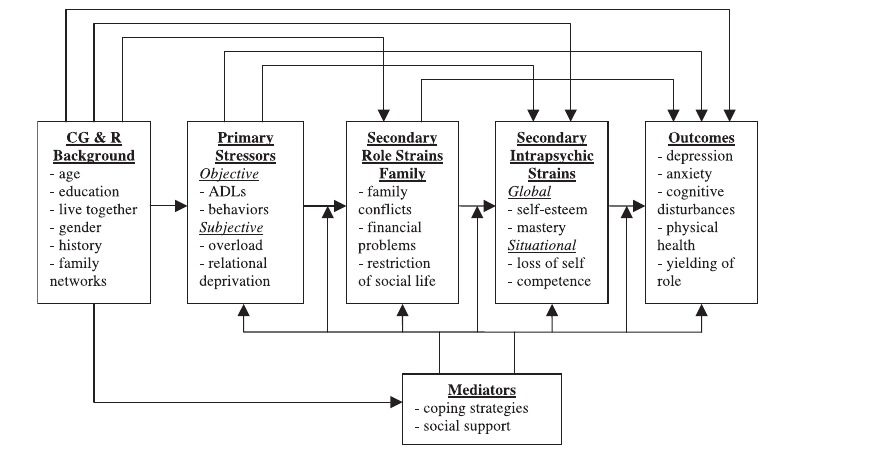
\includegraphics[width=160mm,height=80mm]{./Figures/img_frame}} 
	\caption{El modelo de ansiedad en cuidadores (Pearlin et. al 1990)} \label{fig:modeloAnsiedad}
\end{figure}
El modelo de la ansiedad en cuidadores, es definido por Pearlin como un conjunto de caracter\'isticas del individuo, factores de estres, carga del cuidador y estrategias de afrontamiento, las cuales tienen como salida efectos positivos o negativos\citep{Pearlin01101990}. A continuaci\'on, se explica el modelo de Pearlin elemento por elemento.
	\subsection{Caracter\'isticas del individuo}{\label{secc:modeloAnsiedadCaregivers}}
		La edad y sexo, el nivel de educaci\'on y los lazos que tiene el cuidador con la persona con demencia son los principales factores que pueden hacer mas suceptible a los cuidadores de sufrir los efectos de la ansiedad. Un adolescente que sin experiencia de cuidador podr\'ia sentirse en grandes aprietos al tratar de satisfacer una necesidad de una persona con demencia. De la misma forma, es dif\'icil emocionalmente para los cuidadores ver como el declive cognitivo de un familiar con demencia se va desarrollando hasta el grado de que no reconozca a sus propios hijo.
	\subsection{Factores de estr\'es primarios}{\label{secc:modeloAnsiedadStressFactors}}
		Los factores de estr\'es, o la carga f\'isica y/o cognitiva se dividen en dos: Los factores de estr\'es objetivos y los subjetivos. Los objetivos son aquellos que podemos medir como las actividades de la vida diaria (ADL) y los comportamientos. Estos los podemos medir como la frecuencia y severidad de los eventos en un espacio de tiempo y podemos hacer un registro de ellos. Por otra parte, los subjetivos son aquellos que residen dentro de la mente del cuidador, como la sobrecarga y la deprivaci\'on relacional.
	\subsection{Carga del cuidador}{\label{secc:modeloAnsiedadSecondaryroles}}
		Comunmente, los cuidadores son familiares que viven en la misma casa que la persona con demencia, por lo que suelen tener diferentes roles sociales. Muchos de ellos son madres, padres o hijos que tienen la obligaci\'on de trabajar y proveer de recursos al hogar. La carga extra de cuidar a alguien puede resultar en un desequilibrio emocional del cuidador.
	
	\subsection{Estrategias de afrontamiento}{\label{secc:modeloAnsiedadCoping}}
	Algunos cuidadores logran reducir su nivel de ansiedad por medio de estrategias de afrontamiento. Ejercicios de respiraci\'on, la b\'usqueda de apoyo de familiares y amigos o el consuelo religioso \citep{Sharma20121287} son algunas de las t\'ecnicas que mas sirven a los cuidadores. Sin embargo, no todos ellos las utilizan o utilizan estrategias negativas como el uso de alcohol o drogas.

	La salida de este modelo, afecta en los niveles de depresi\'on, ansiedad y salud f\'isica del cuidador. El buen uso de las estrategias de afrontamiento, el balance de roles y carga del cuidador pueden ayudar a reducir su ansiedad y mejorar su salud f\'isica y/o mental.

	\subsection{Cuidadores Formales e Informales}\label{secc:caregivers}


	\subsection{Se\~nales fisiol\'ogicas relacionadas}\label{secc:signals}
	El Sistema Aut\'onomo Central (SAC) es una divisi\'on del Sistema Nervioso Perif\'erico (SNP) el cual controla el funcionamiento de los \'organos viscerales. Controla las funciones del cuerpo como la respiraci\'on, digesti\'on, ritmo cardi\'aco, y deseo sexual de manera inconsciente. Est\'a dividido por dos subsistemas: el \textit{Sistema Nervioso Simp\'atico} y el \textit{Sistema Nervioso Parasimp\'atico} (Ver Figura ~\ref{fig:modeloSNP}). Ambos controlan las mismas funciones, pero de manera an\'aloga. Mientras el SNS aumenta los latidos del coraz\'on, el SNP lo disminuye..

\begin{figure}[h]
	\centering
	\subfigure[]{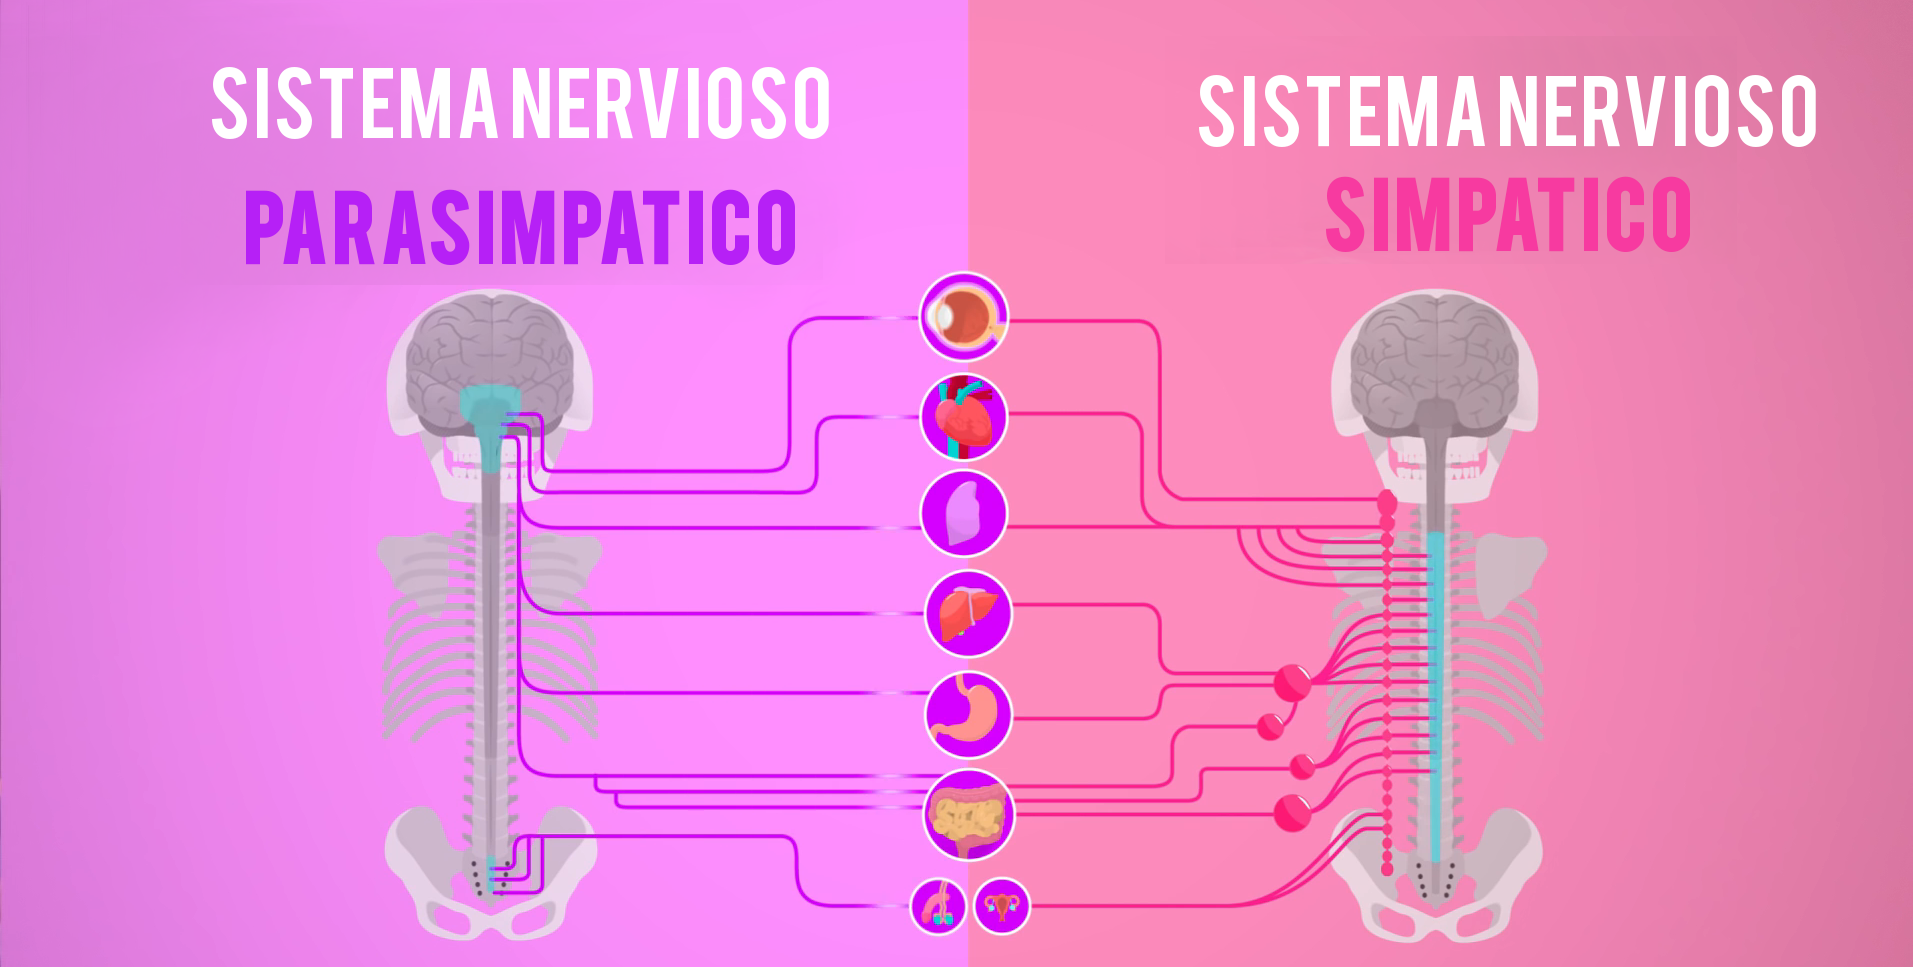
\includegraphics[width=160mm,height=80mm]{./Figures/img_snc}} 
	\caption{El sistema Aut\'onomo central (Crash Course A\&P \#13) \label{fig:modeloSNP}}
\end{figure}

Los efectos de la ansiedad se manifestan en el ritmo card\'iaco [ref], respiraci\'on [ref] y sudoraci\'on [ref] los cuales son controlados por el SAC. Normalmente, el individuo no tiene control sobre los cambios en sus funciones corporales. A continuaci\'on, se explican las diferentes se\~nales usadas para detectar la ansiedad.

	\subsubsection{Respuesta Galv\'anica de la Piel (GSR)}\label{secc:gsr}
	Uno de los efectos que la ansiedad causa sobre el cuerpo es la sudoraci\'on. El sudor est\'a formado mayormente por agua y minerales y ayuda a mantener la temperatura corporal. Un efecto secundario de la presencia del sudor es el cambio en la conductancia el\'ectrica de la piel, siendo esta definida como \textit{``la facilidad que ofrece un material apaso de la corrente el\'ectrica''}. Esta capacidad de conductividad es denotada por la unidad del sistema internacional \textit{Siemen ($S$)}. La unidad $S$ est\'a definida por: $S = \Omega^{-1} = \dfrac{A}{V}$. Donde $\Omega$ es el ohm, $A$ es el ampero y $V$ es el Voltio. Debido a que los valores de las mediciones son comunmente muy peque\~nas, las mediciones son denotadas por el prefijo $\mu$.
	\begin{figure}[h]
		\centering
		\subfigure[]{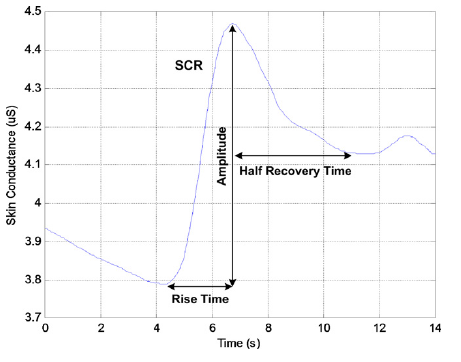
\includegraphics[width=100mm,height=80mm]{./Figures/img_gsr}} 
		\caption{Se\~nal t\'ipica de GSR \label{fig:GSRsignal}}
	\end{figure}

	La se\~nal de GSR se encuentra compuesta por dos partes: Un componente base y un componente t\'onico \citep{Katsis2011261}. El componente base corresponde a un nivel promedio sin un \textit{stimuli} en concreto, mientras que el componente t\'onico es la reacci\'on a un est\'imulo. La figura ~\ref{fig:GSRsignal} ejemplifica ambos componentes. Los picos durante el componente t\'onico tiene las siguientes caracter\'isticas:

\begin{itemize}
        \item{\textbf{Tiempo de Levantamiento del pico:}} Es el tiempo que tarda la se\~nal en alcanzar el punto m\'aximo (pico) en el segmento.
        \item{\textbf{Amplitud del pico:}} Es el valor de la se\~nal en el pico.
        \item{\textbf{Tiempo de media recuperac\'on :}} Es el tiempo que tarda la se\~nal en disminuir la mitad del valor de la amplitud del pico.
\end{itemize}


	\subsubsection{Se\~nales relacionadas con el coraz\'on}\label{secc:hearthrate}
	Las se\~nales relacionadas con el coraz\'on son utilizadas ampliamente como indicadores principales en estudios de detecci\'on de ansiedad y estr\'es [ref]. A continuaci\'on se describen algunas de ellas:
	\begin{itemize}
		\item \textit{Ritmo Card\'iaco (HR):} Se define como el n\'umero de latidos por minuto (BPM).
		\item \textit{Intervalo entre latidos (IBI):} Se define como el tiempo en segundos entre un latido y otro. Esta se\~nal est\'a directamente relacionada con el ritmo card\'iaco. Entre menor sea el valor de IBI, mayor ser\'a el valor del HR.
	\end{itemize}
	\subsubsection{Electroencefalogram\'ia (EEG)}\label{secc:eeg}

\section{Instrumentos tradicionales para la medici\'on de la ansiead}
        En psicolog\'ia existen diversos instrumentos que permiten detectar la ansiedad. Algunos de los cuestionarios existentes son:
        \begin{itemize}

                \item Hamilton Anxiety Rating Scale

                \item Zung Self-Rating Anxiety Scale (SAS)

                \item The State-Trait Anxiety Inventory (STAI)
                \item Subjective Self-raiting Anxiety Scale (SUDS)
        \end{itemize}


\section{C\'omputo vestible}\label{secc:dementia}
El c\'omputo vestible nos permite llevar computadoras con nosotros de la misma manera que llevamos la ropa puesta. Al ``vestir'' un dispositivo, el usuario tiene acceso a una computadora que es capaz de monitorearlo a \'el y a su entorno por medio de sensores. Los sensores pueden medir entre otras cosas: movimientos del cuerpo del usuario, la posici\'on del usuario, intensidad de luz, ruido, im\'agenes de su ambiente, ritmo card\'iaco, capacidad conductiva de la piel, distancias, actividad cerebral, entre otros. Debido a la cercania con el usuario, se pueden hacer monitoreos constantes y mas precisos que con los sistemas tradicionales y ayudar en las tareas de la vida cotidiana.

El uso de c\'omputo vestible abre la posibilidad de detectar la ansiedad por medio de las se\~nales fisiol\'ogicas del usuario.

\section{Trabajo previo en detecci\'on de ansiedad}

Existen diferentes estudios sobre detecci\'on de ansiedad.
*Trabajos de Bert
*Trabajos que encontre

\section{Conclusion}\label{secc:conclution}
El entendimiento del modelo del cuidador y la persona con demencia, las se\~nales del cuerpo y el uso de tecnolog\'ias vestibles, abren la posibilidad de cuantificar estados mentales que en el pasado eran dif\'iciles de medir. El uso de esta informaci\'on y la comunicaci\'on adecuada con el usuario, permitir\'ia la reducci\'on de ansiedad y mejorar el bienestar general del cuidador.

\newpage
%%=====================================================
} }%
%BeginExpansion
\chapter{Fundamentos te\'oricos}\label{capit:cap2}
\vspace{-2.0325ex}%
\noindent
\rule{\textwidth}{0.5pt}
\vspace{-5.5ex}% 
\newcommand{\pushline}{\Indp}% Indent puede ir o no :p

\section{Introducci\'on}\label{secc:introduccion}
La ansiedad es un fen\'omeno con el que nuestra sociedad se encuentra \'intimamente relacionada. Todos la sentimos multiples veces a lo largo de nuestras vidas, al dar un discurso en p\'ublico, al ser entrevistado para un nuevo trabajo o durante un examen. Es parte de lo que nos mantiene alertas y listos para enfrentar las situaciones de d\'ia a d\'ia. Sin embargo, solemos no darle la importancia que significa para las personas que sufren de elevados niveles de ansiedad y de los beneficios que la tecnolog\'ia puede brindarles. En este cap\'itulo, se define la ansiedad, la manera en que se origina, como afecta a los cuidadores y como podemos medirla.



\section{Qu\'e es la Ansiedad?}\label{secc:ansiedad}

La ansiedad es una emoci\'on caracterizada por sensaciones de tensi\'on, pensamientos de preocupaci\'on y cambios f\'isicos como incremento en la presi\'on arterial \citep{psychologyapa}, aumento de la sudoraci\'on y palpitaciones, entre otras respuestas fisiol\'ogicas. Estas manifestaciones se dan en determinados lapsos de tiempos durante la vida del individuo. Durante estos lapsos, se dice que el sujeto se encuentra en un estado mental de ansiedad [ref].

Este estado mental es \'util para los humanos, debido a que la ansiedad es una reacci\'on normal del cuerpo para lograr objetivos, o lograr sobrevivir ante a una amenaza. Sin embargo, cuando la persona experimenta un nivel de ansiedad el cual es tan alto que no le permite manejar su vida normal, se dice que la persona tiene un desorden de ansiedad\citep{repetto2013}. 

\subsection{Ansiedad y estr\'es}\label{secc:anxietyandstress}
Si bien, en ocasiones el estr\'es y la ansiedad son conceptos que se usan de manera intercambiable, existen diferencias entre ambos. El estr\'es es definido como el desvalance entre la carga mental dada y la percepci\'on de las habilidades que el individuo tiene para lidiar dicha carga[ref]. Este desvalance puede hacer que la ansiedad aumente, mientras que la ansiedad puede a su vez generar estr\'es. La relaci\'on entre el estr\'es y la ansiedad es la ansiedad es la se\~nal psicofisiol\'ogica de que la respuesta al estr\'es ha sido iniciada \citep{PMID2235645}.


\subsection{``State Anxiety'' y ``Trait Anxiety''}\label{secc:anxieystatevstrait}
Existen dos clasificaciones de ansiedad reconocidas por la \textit{American Psychological Association} \citep{psychologyapa} , ``State Anxiety'' y ``Trait Anxiety'' las cuales se mencionan a continuaci\'on.

\begin{itemize}
	\item{\textbf{State Anxiety:}} Es una manifestaci\'on de ansiedad a cerca de un evento \textbf{presente} bien definido. Normalmente la persona se encuentra conciente de la fuente de su ansiead. 
	\item{\textbf{Trait Anxiety:}} Es una manifestaci\'on a largo plazo de la ansiedad, en la que el individuo puede entrar al estado de ansiedad sin saber la raz\'on concreta. Las personas con personalidades t\'imidas tienden a sufrir mas de este tipo de ansiedad. [ref]

\end{itemize}

A pesar de que los efectos negativos en la calidad de vida de las personas que sufren de ``Trait Anxiety'' son mas fuertes, este trabajo est\'a enfocado en ``State Anxiety'' debido a que es mas f\'acil de cuantificar y medir por medio de sensores.

\section{Demencia}\label{secc:dementia}
La demencia es un s\'indrome del declive de las habilidades cognitivas. Los s\'intomas comunes son: problemas de memoria, dificultades para realizar tareas familiares, mal juicio, deterioro del lenguaje hablado y cambios de humor\citep{Aziz}. Afecta alrededor de el 4\% de las personas mayores de 65 a\~nos y al 40\% de las personas mayores de 90. La demencia suele manifestarse en sindromes como el de Alzheimer. Las personas con demencia necesitan de una persona que cuide de ellos, normalmente durante el resto de su vida. Usualmente necesitan ayuda en las actividades de la vida diaria (Activities of Daily Life), siendo esto una carga para los cuidadores.

\section{Cuidadores}\label{secc:caregivers}
Uno de los sectores de poblaci\'on vulnerables, son los cuidadores de personas con demencia. Se encuentra documentado que los cuidadores, al llevar una carga f\'isica, cognitiva y emocional derivada de su labor les genera padecimientos como ansiedad, estr\'es, y hasta la muerte\citep{Chen2013}. Debido a que los cuidadores no necesariamente son personas con una formaci\'on profesional, estos efectos pueden verse aumentados. Por lo general, los cuidadores que son familiares del paciente son a\'un m\'as afectados ya que necesitan administrar el tiempo de trabajo, familia, actividades sociales y la actividad misma del cuidado del paciente.
			%Cuales son las situaciones ( escenarios ) en los que los CUIDADORES presentan ansiedad?

\subsection{C\'omo se genera la ansiedad en los cuidadores?}\label{secc:caregiverburden}

\begin{figure}[h]
	\centering
	\subfigure[]{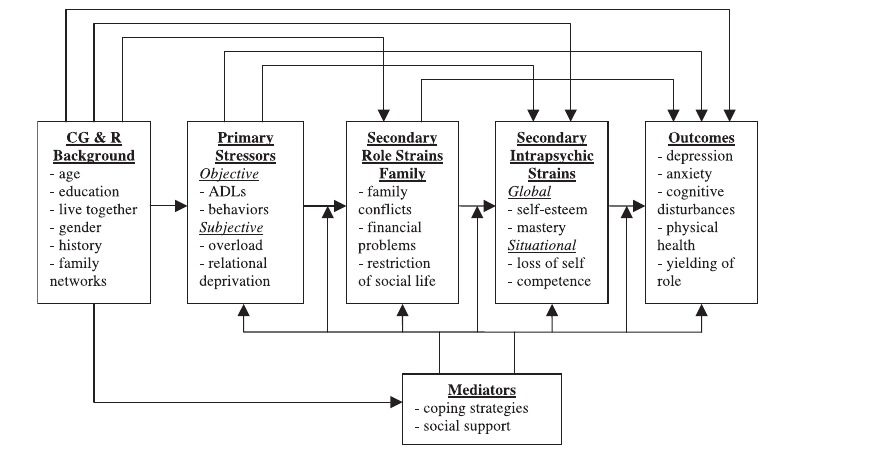
\includegraphics[width=160mm,height=80mm]{./Figures/img_frame}} 
	\caption{El modelo de ansiedad en cuidadores (Pearlin et. al 1990)} \label{fig:modeloAnsiedad}
\end{figure}
El modelo de la ansiedad en cuidadores, es definido por Pearlin como un conjunto de caracter\'isticas del individuo, factores de estres, carga del cuidador y estrategias de afrontamiento, las cuales tienen como salida efectos positivos o negativos\citep{Pearlin01101990}. A continuaci\'on, se explica el modelo de Pearlin elemento por elemento.
	\subsection{Caracter\'isticas del individuo}{\label{secc:modeloAnsiedadCaregivers}}
		La edad y sexo, el nivel de educaci\'on y los lazos que tiene el cuidador con la persona con demencia son los principales factores que pueden hacer mas suceptible a los cuidadores de sufrir los efectos de la ansiedad. Un adolescente que sin experiencia de cuidador podr\'ia sentirse en grandes aprietos al tratar de satisfacer una necesidad de una persona con demencia. De la misma forma, es dif\'icil emocionalmente para los cuidadores ver como el declive cognitivo de un familiar con demencia se va desarrollando hasta el grado de que no reconozca a sus propios hijo.
	\subsection{Factores de estr\'es primarios}{\label{secc:modeloAnsiedadStressFactors}}
		Los factores de estr\'es, o la carga f\'isica y/o cognitiva se dividen en dos: Los factores de estr\'es objetivos y los subjetivos. Los objetivos son aquellos que podemos medir como las actividades de la vida diaria (ADL) y los comportamientos. Estos los podemos medir como la frecuencia y severidad de los eventos en un espacio de tiempo y podemos hacer un registro de ellos. Por otra parte, los subjetivos son aquellos que residen dentro de la mente del cuidador, como la sobrecarga y la deprivaci\'on relacional.
	\subsection{Carga del cuidador}{\label{secc:modeloAnsiedadSecondaryroles}}
		Comunmente, los cuidadores son familiares que viven en la misma casa que la persona con demencia, por lo que suelen tener diferentes roles sociales. Muchos de ellos son madres, padres o hijos que tienen la obligaci\'on de trabajar y proveer de recursos al hogar. La carga extra de cuidar a alguien puede resultar en un desequilibrio emocional del cuidador.
	
	\subsection{Estrategias de afrontamiento}{\label{secc:modeloAnsiedadCoping}}
	Algunos cuidadores logran reducir su nivel de ansiedad por medio de estrategias de afrontamiento. Ejercicios de respiraci\'on, la b\'usqueda de apoyo de familiares y amigos o el consuelo religioso \citep{Sharma20121287} son algunas de las t\'ecnicas que mas sirven a los cuidadores. Sin embargo, no todos ellos las utilizan o utilizan estrategias negativas como el uso de alcohol o drogas.

	La salida de este modelo, afecta en los niveles de depresi\'on, ansiedad y salud f\'isica del cuidador. El buen uso de las estrategias de afrontamiento, el balance de roles y carga del cuidador pueden ayudar a reducir su ansiedad y mejorar su salud f\'isica y/o mental.

	\subsection{Cuidadores Formales e Informales}\label{secc:caregivers}


	\subsection{Se\~nales fisiol\'ogicas relacionadas}\label{secc:signals}
	El Sistema Aut\'onomo Central (SAC) es una divisi\'on del Sistema Nervioso Perif\'erico (SNP) el cual controla el funcionamiento de los \'organos viscerales. Controla las funciones del cuerpo como la respiraci\'on, digesti\'on, ritmo cardi\'aco, y deseo sexual de manera inconsciente. Est\'a dividido por dos subsistemas: el \textit{Sistema Nervioso Simp\'atico} y el \textit{Sistema Nervioso Parasimp\'atico} (Ver Figura ~\ref{fig:modeloSNP}). Ambos controlan las mismas funciones, pero de manera an\'aloga. Mientras el SNS aumenta los latidos del coraz\'on, el SNP lo disminuye..

\begin{figure}[h]
	\centering
	\subfigure[]{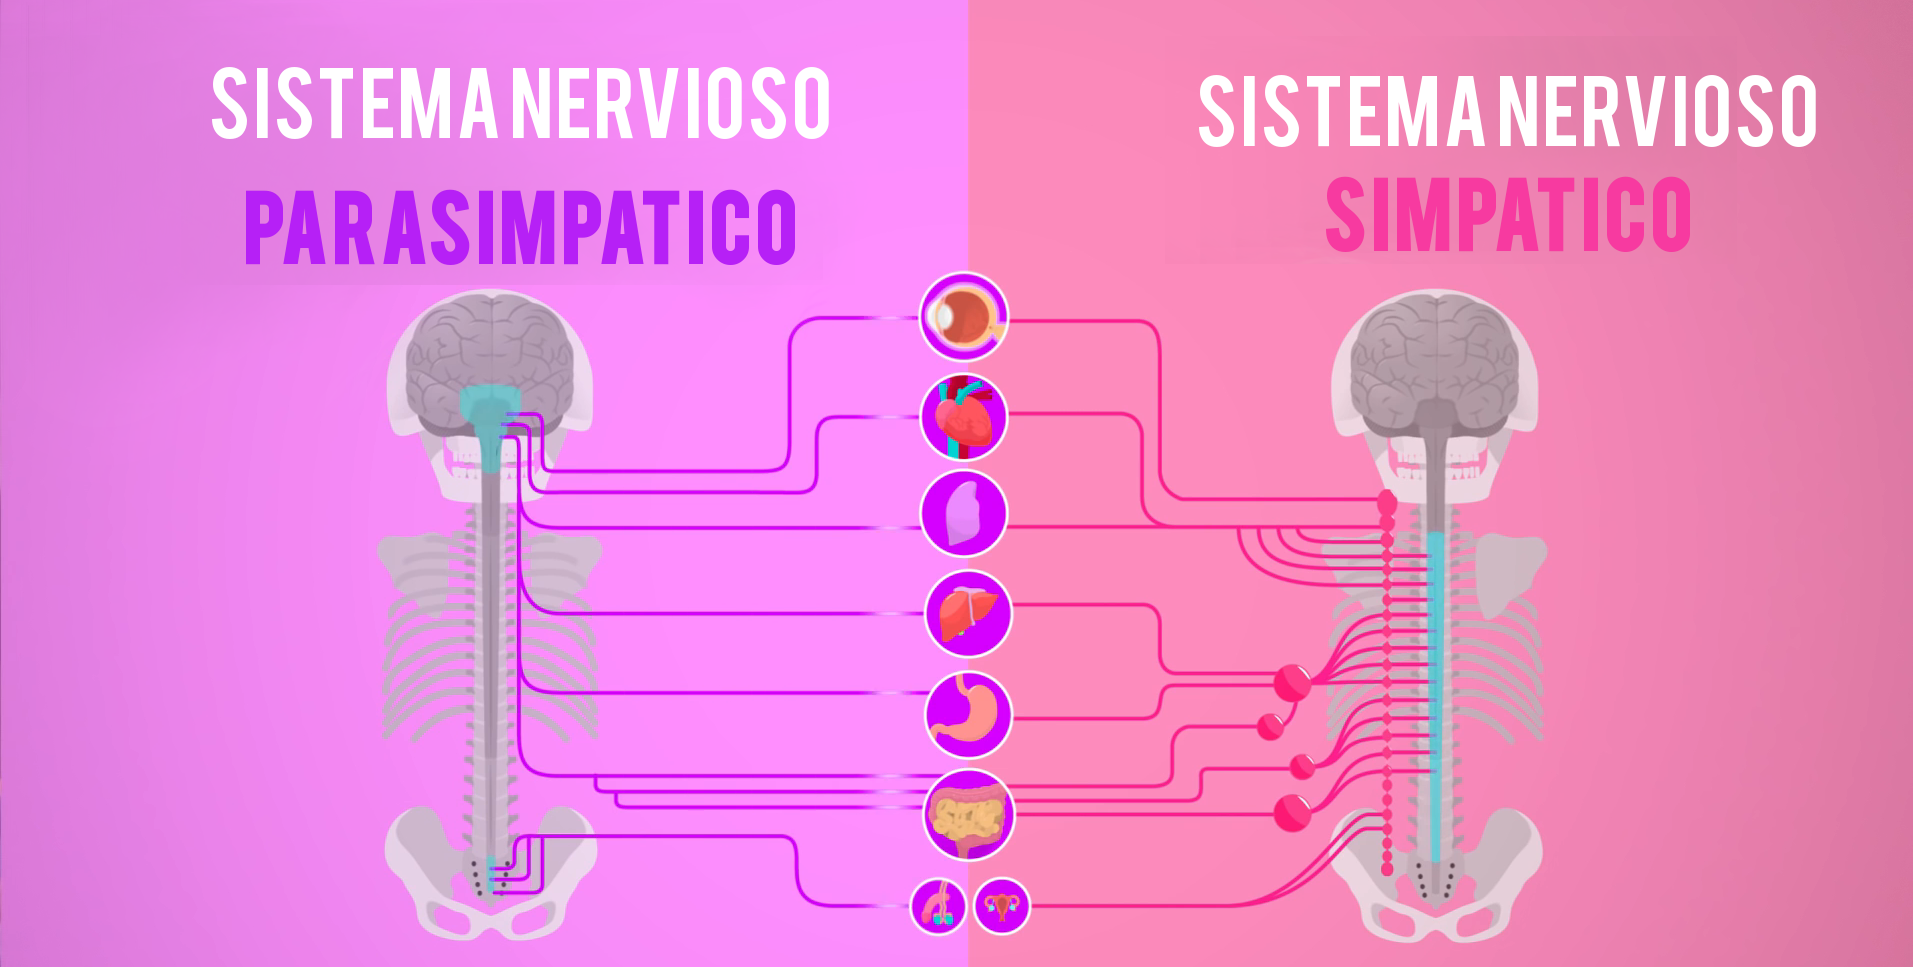
\includegraphics[width=160mm,height=80mm]{./Figures/img_snc}} 
	\caption{El sistema Aut\'onomo central (Crash Course A\&P \#13) \label{fig:modeloSNP}}
\end{figure}

Los efectos de la ansiedad se manifestan en el ritmo card\'iaco [ref], respiraci\'on [ref] y sudoraci\'on [ref] los cuales son controlados por el SAC. Normalmente, el individuo no tiene control sobre los cambios en sus funciones corporales. A continuaci\'on, se explican las diferentes se\~nales usadas para detectar la ansiedad.

	\subsubsection{Respuesta Galv\'anica de la Piel (GSR)}\label{secc:gsr}
	Uno de los efectos que la ansiedad causa sobre el cuerpo es la sudoraci\'on. El sudor est\'a formado mayormente por agua y minerales y ayuda a mantener la temperatura corporal. Un efecto secundario de la presencia del sudor es el cambio en la conductancia el\'ectrica de la piel, siendo esta definida como \textit{``la facilidad que ofrece un material apaso de la corrente el\'ectrica''}. Esta capacidad de conductividad es denotada por la unidad del sistema internacional \textit{Siemen ($S$)}. La unidad $S$ est\'a definida por: $S = \Omega^{-1} = \dfrac{A}{V}$. Donde $\Omega$ es el ohm, $A$ es el ampero y $V$ es el Voltio. Debido a que los valores de las mediciones son comunmente muy peque\~nas, las mediciones son denotadas por el prefijo $\mu$.
	\begin{figure}[h]
		\centering
		\subfigure[]{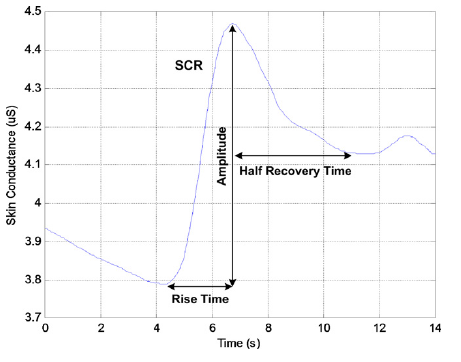
\includegraphics[width=100mm,height=80mm]{./Figures/img_gsr}} 
		\caption{Se\~nal t\'ipica de GSR \label{fig:GSRsignal}}
	\end{figure}

	La se\~nal de GSR se encuentra compuesta por dos partes: Un componente base y un componente t\'onico \citep{Katsis2011261}. El componente base corresponde a un nivel promedio sin un \textit{stimuli} en concreto, mientras que el componente t\'onico es la reacci\'on a un est\'imulo. La figura ~\ref{fig:GSRsignal} ejemplifica ambos componentes. Los picos durante el componente t\'onico tiene las siguientes caracter\'isticas:

\begin{itemize}
        \item{\textbf{Tiempo de Levantamiento del pico:}} Es el tiempo que tarda la se\~nal en alcanzar el punto m\'aximo (pico) en el segmento.
        \item{\textbf{Amplitud del pico:}} Es el valor de la se\~nal en el pico.
        \item{\textbf{Tiempo de media recuperac\'on :}} Es el tiempo que tarda la se\~nal en disminuir la mitad del valor de la amplitud del pico.
\end{itemize}


	\subsubsection{Se\~nales relacionadas con el coraz\'on}\label{secc:hearthrate}
	Las se\~nales relacionadas con el coraz\'on son utilizadas ampliamente como indicadores principales en estudios de detecci\'on de ansiedad y estr\'es [ref]. A continuaci\'on se describen algunas de ellas:
	\begin{itemize}
		\item \textit{Ritmo Card\'iaco (HR):} Se define como el n\'umero de latidos por minuto (BPM).
		\item \textit{Intervalo entre latidos (IBI):} Se define como el tiempo en segundos entre un latido y otro. Esta se\~nal est\'a directamente relacionada con el ritmo card\'iaco. Entre menor sea el valor de IBI, mayor ser\'a el valor del HR.
	\end{itemize}
	\subsubsection{Electroencefalogram\'ia (EEG)}\label{secc:eeg}

\section{Instrumentos tradicionales para la medici\'on de la ansiead}
        En psicolog\'ia existen diversos instrumentos que permiten detectar la ansiedad. Algunos de los cuestionarios existentes son:
        \begin{itemize}

                \item Hamilton Anxiety Rating Scale

                \item Zung Self-Rating Anxiety Scale (SAS)

                \item The State-Trait Anxiety Inventory (STAI)
                \item Subjective Self-raiting Anxiety Scale (SUDS)
        \end{itemize}


\section{C\'omputo vestible}\label{secc:dementia}
El c\'omputo vestible nos permite llevar computadoras con nosotros de la misma manera que llevamos la ropa puesta. Al ``vestir'' un dispositivo, el usuario tiene acceso a una computadora que es capaz de monitorearlo a \'el y a su entorno por medio de sensores. Los sensores pueden medir entre otras cosas: movimientos del cuerpo del usuario, la posici\'on del usuario, intensidad de luz, ruido, im\'agenes de su ambiente, ritmo card\'iaco, capacidad conductiva de la piel, distancias, actividad cerebral, entre otros. Debido a la cercania con el usuario, se pueden hacer monitoreos constantes y mas precisos que con los sistemas tradicionales y ayudar en las tareas de la vida cotidiana.

El uso de c\'omputo vestible abre la posibilidad de detectar la ansiedad por medio de las se\~nales fisiol\'ogicas del usuario.

\section{Trabajo previo en detecci\'on de ansiedad}

Existen diferentes estudios sobre detecci\'on de ansiedad.
*Trabajos de Bert
*Trabajos que encontre

\section{Conclusion}\label{secc:conclution}
El entendimiento del modelo del cuidador y la persona con demencia, las se\~nales del cuerpo y el uso de tecnolog\'ias vestibles, abren la posibilidad de cuantificar estados mentales que en el pasado eran dif\'iciles de medir. El uso de esta informaci\'on y la comunicaci\'on adecuada con el usuario, permitir\'ia la reducci\'on de ansiedad y mejorar el bienestar general del cuidador.

\newpage
%%=====================================================

%EndExpansion
\newpage }

{\normalsize
%TCIMACRO{\QSubDoc{Include Capitulo03}{\chapter{Dise\~no de un estudio de usuario para inducir ansiedad en cuidadores de personas con demencia}\label{capit:cap3}
\vspace{-2.0325ex}%
\noindent
\rule{\textwidth}{0.5pt}
\vspace{-5.5ex}% 
\newcommand{\pushline}{\Indp}% Indent puede ir o no :p
\section{Introducci\'on}\label{secc:introduction}

Como vimos en el cap\'itulo 2, la mayor\'ia de los estudios logran inducir ansiedad o estr\'es por medio de situaciones controladas dentro del laboratorio. Sin embargo, generar ansiedad en cuidadores informales es mucho mas dif\'icil. El escenario de un laboratorio no coincide con el entorno en el que una persona con demencia se desarrolla, por lo que los comportamientos impredecibles no ser\'ian congruentes con dicho ambiente. Adem\'as, exponer a personas sin experiencia ante una persona con demencia que tiene necesidades reales resultar\'ia riesgoso para ambos individuos. Por otra parte, realizar una intervenci\'on totalmente natural a\~nade un grado de dificultad al estudio, resultando en ruido en los datos recolectados (p. ej. la se\~nal de ritmo card\'iaco podr\'ia ser alta no por una situaci\'on de ansiedad, sino por una actividad f\'isica, m\'ultiples distracciones o responsabilidades al mismo tiempo para el cuidador) haciendo d\'ificil de analizarlos.

En este cap\'itulo se explica el uso de una t\'ecnica llamada ``Naturalistic Enactment (NE)'' \citep{Castro11} dentro de un estudio de usuario para capturar datos de ansiedad en cuidadores de personas con demencia.


\section{Un estudio de usuario para inducir ansiedad en cuidadores informales}\label{secc:experiment}
Se dise\~n\'o un estudio de usuario para inducir ansiedad en cuidadores informales bajo situaciones simuladas y parecidas a la realidad. Para lograr esto, se utiliz\'o la t\'ecnica de NE. NE fue propuesta originalmente para evaluar tecnolog\'ias m\'edicas ubicuas, donde el tener una validez ambiental e interacc\'on directa del usuario es importante, y donde sin embargo, utilizar pacientes reales puede ser peligroso \citep{Castro11}. NE consiste del desarrollo de tareas reales (p. ej. la exposici\'on a situaciones y tareas en situaciones naturales) para simular la experiencia del usuario bajo condiciones normales, y por lo tanto encontrar problemas y comportamientos que pudieran de otra manera haber sido dif\'iciles de capturar. NE representa una ventaja ante otros m\'etodos de evaluaci\'on gracias a su alta fidelidad, mediano riesgo y alta involucramiento del usuario (Ver figura ~\ref{fig:evalmethods}).

\begin{figure}[h]
        \centering
        \subfigure[]{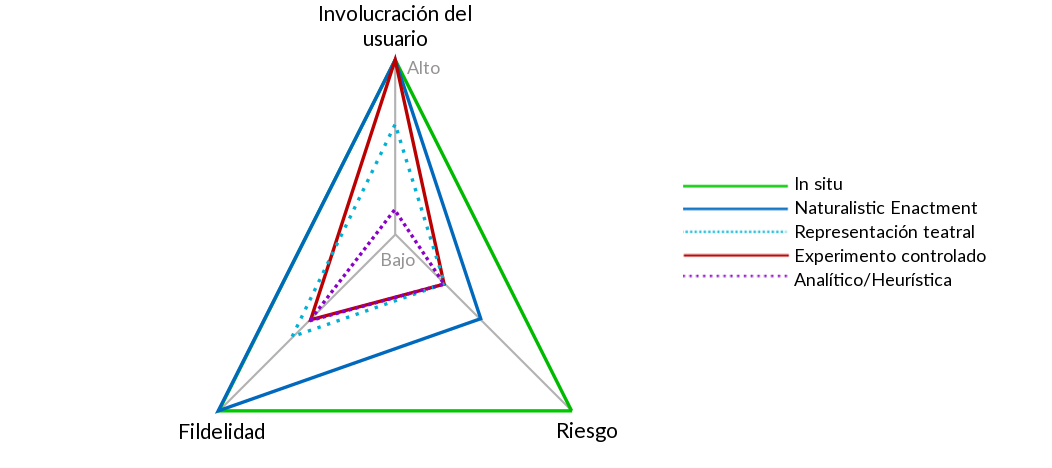
\includegraphics[width=160mm]{./Figures/img_evalmethods}}
	\caption{M\'etodos de evaluaci\'on clasificados de acuerdo a la involucramiento del usuario, fidelidad y riesgo \protect\citep{Castro11} }\label{fig:evalmethods}
\end{figure}


Para poder exponer a los sujetos a una situaci\'on de cuidador, estresante y realista, bajo condiciones controladas; se formul\'o un ejercicio que consisti\'o de una situaci\'on de terapia real con una persona actuando como si tuviera demencia. Un adulto mayor de 75 a\~nos actu\'o como si sufriera de demencia. Una especialista en intervenciones con adultos mayores con demencia le entren\'o con los comportamientos t\'ipicos de demencia moderada como: murmureo, gritos, vagabundeo, preguntas repetitivas, entre otras. Ella ya estaba familiarazada con estos comportamientos por conocidos que sufrieron de demencia. En cambio, se les dijo que se evaluaba su rendimiento como cuidadores basados en el entrenamiento inicial que se les di\'o. Para fines pr\'acticos de esta tesis, se referir\'a al adulto mayor como actor de un adulto mayor con demencia (aPcD).

Se les pidi\'o firmar un documento de no divulgaci\'on (Ver Ap\'endice~\ref{aped:cartanodiv}) para evitar que los participantes hablaran entre ellos acerca del estudio de usuario, de los comportamientos del adulto mayor o cualquier otra t\'ecnica acerca de como manejar el comportamiento del adulto mayor, durante el tiempo en que el estudio de usuario durara.

\subsection{Participantes}\label{secc:subjects}
Los sujetos fueron reclutados a trav\'es de la lista de correo de CICESE (3 personas), por el departamento de ciencias de la computaci\'on (5 personas) y dos personas externas a la instituci\'on. Se les otorg\'o un premio de compensaci\'on de 100.00 MXN en dinero electr\'onico para el cine. Se les pidi\'o a los participantes asisitr a 3 sesiones (una por cada semana), cada sesi\'on dur\'o al rededor de 30 minutos. Para simular el escenario de una persona que reci\'en toma un papel de cuidador se excluyeron a personas que fueran cuidadores que fueran cuidadores en el momento. Se incluyeron a personas que tuvieran experiencia previa como cuidadores informales para realizar comparaciones futuras (ver Trabajo a futuro). Se les dijo que estar\'ian trabajando con una persona que realmente ten\'ia demencia. Tambi\'en, se les ocult\'o la verdadera raz\'on del estudio. Se obtuvo consentimiento firmado de todos los sujetos (Ver Ap\'endice ~\ref{aped:cartainfo})

Todos los sujetos participaron en una sesi\'on de entrenamiento, en donde una especialista en intervenciones con adultos mayores con demencia les explic\'o las actividades a realizar en las terapias que hicieron con el adulto mayor.
Participaron 10 estudiantes (5 hombres y 5 Mujeres) con un promedio de 24.5 a\~nos de edad ($\sigma=1.059$). La tabla \ref{table:kysymys} muestra los datos demogr\'aficos de los participantes.
\begin{table}
	\footnotesize
	\centering
	\caption{Participantes en el estudio}
	\label{table:kysymys}
	%\rotatebox{90}{
	\begin{tabular}{m{0.2cm}m{2.5cm}m{2.5cm}m{2.5cm}m{2.5cm}}
		\hline\noalign{\smallskip}
		 & \textbf{Sujeto} & \textbf{G\'enero} & \textbf{Edad} & \textbf{Experiencia de cuidador}
		\\ \noalign{\smallskip}
		\hline
		\noalign{\smallskip}
		&S1& Masculino & 24 & No   \\ 
		&S2& Masculino &  25&  No  \\ 
		&S3& Femenino & 24 & No   \\ 
		&S4& Femenino & 26 & No  \\ 
		&S5& Femenino & 24 & No   \\ 
		&S6& Masculino & 26 &  No  \\ 
		&S7& Masculino & 23 &  No \\ 
		&S8& Masculino & 25 &  Si  \\ 
		&S9& Femenino & 26 & No   \\ 
	  	&S10& Femenino & 24 & Si  \\ 
		\hline
	\end{tabular}
	%}
\end{table}
\section{Procedimiento}\label{secc:methods}
El desarrollo del estudio de usuario se dividi\'o en diferentes actividades. A continuaci\'on se explican a detalle cada una de ellas.
\subsection{Entrenamiento}\label{secc:training}
	Todos los sujetos participaron en una sesi\'on de entrenamiento para familiarizarse con las terapias cognitivas que har\'ian con el adulto mayor. La sesi\'on de entrenamiento dur\'o aproximadamente 90 minutos. Todos los participantes practicaron las terapias y tuvieron oportunidad de hacer preguntas. No se les di\'o ninguna estrategia de afrontamiento acerca de como lidiar con los comportamientos del adulto mayor. Se les dijo a los participantes que el adulto mayor ten\'ia declive cognitivo ligero y que podr\'ia mostrar algunos problemas de comportamiento como olvidar instrucciones recientes, apat\'ia y renuencia de completar las tareas, entre otras. Se les dijo que las tareas no ten\'ian que ser completadas si el adulto mayor no estaba cooperando, pero que deber\'ian intentar completar la terap\'ia.

\subsection{Tareas de terapias}\label{secc:therapytasks}
Antes de iniciar la tarea, equipamos a los participantes con una banda de pecho Zephyr Hxm para monitorear su ritmo card\'iaco, una pulsera Empatica E3 para obtener GSR y temperatura corporal y una banda cerebral Muse para obtener datos de EEG. Todas las sesiones fueron videograbadas para analizarlas posteriormente.

Durante cinco minutos y ya equipados con los dispositivos, se les pidi\'o a los participantes relajarase por medio de respiraci\'on profunda y con los ojos cerrados para obtener una l\'inea base de datos fisiol\'ogicos. S\'olo una persona necesit\'o mas de 5 minutos debido a que tuvo problemas para relajarse.

Se les pidi\'o a los participantes que guiaran al adulto mayor a trav\'es de una sesi\'on de terapia que involucr\'o una de las 7 posibles tareas que fueron explicadas durante la sesi\'on de entrenamiento. La tabla ~\ref{table:therapies} presenta las tareas realizadas por cada participante en las tres sesiones del estudio. La figura ~\ref{fig:imgtherapies} muestra dos terapias de ejemplo. Los rostros de los participantes fueron modificados para mantener su privacidad.

\begin{table}[h!]
	\footnotesize
	\centering
	\caption{Terapias realizadas con el adulto mayor por cada participante.}
	\label{table:therapies}
	%\rotatebox{90}{
	\renewcommand{\arraystretch}{1.5}
	\begin{tabular}{m{0.2cm}m{3.5cm}m{3.5cm}m{3.5cm}m{3.5cm}}
		\hline\noalign{\smallskip}
	&\textbf{Participante}&  \textbf{Terapia 1}& \textbf{Terapia 2}   & \textbf{Terapia 3}  \\ \hline
		\\ \noalign{\smallskip}
		&S1&  Atado de agujetas& Memorama & \pbox{12cm}{Clasificaci\'on\\de im\'agenes}   \\ 
  &S2&  \pbox{12cm}{Clasificaci\'on\\de im\'agenes}& Atado de agujetas & Crucigrama   \\ 
  &S3&  \pbox{12cm}{Formaci\'on de palabras}& Cruzigrama & Memorama    \\ 
  &S4&  Atado de agujetas&\pbox{12cm}{Clasificaci\'on de\\im\'agenes}& Memorama   \\ 
  &S5&  \pbox{12cm}{Clasificaci\'on\\de im\'agenes}&  Atado de agujetas & Crucigrama   \\ 
  &S6&  \pbox{12cm}{Separaci\'on de objetos}& Memorama & Atado de agujetas   \\ 
  &S7&  \pbox{12cm}{Separaci\'on de objetos}& Atado de agujetas & Crucigrama   \\ 
  &S8&  Crucigrama& Atado de agujetas &\pbox{12cm}{Clasificaci\'on\\de im\'agenes}   \\ 
  &S9&  \pbox{12cm}{Formaci\'on\\de palabras}& \pbox{12cm}{Clasificaci\'on\\de im\'agenes} & Memorama   \\ 
  &S10&  Memorama&\pbox{12cm}{Formaci\'on\\de palabras} & Atado de agujetas   \\ 
		\hline
	\end{tabular}
	%}
\end{table}

\begin{figure}[h!]
        \centering
	\subfigure[]{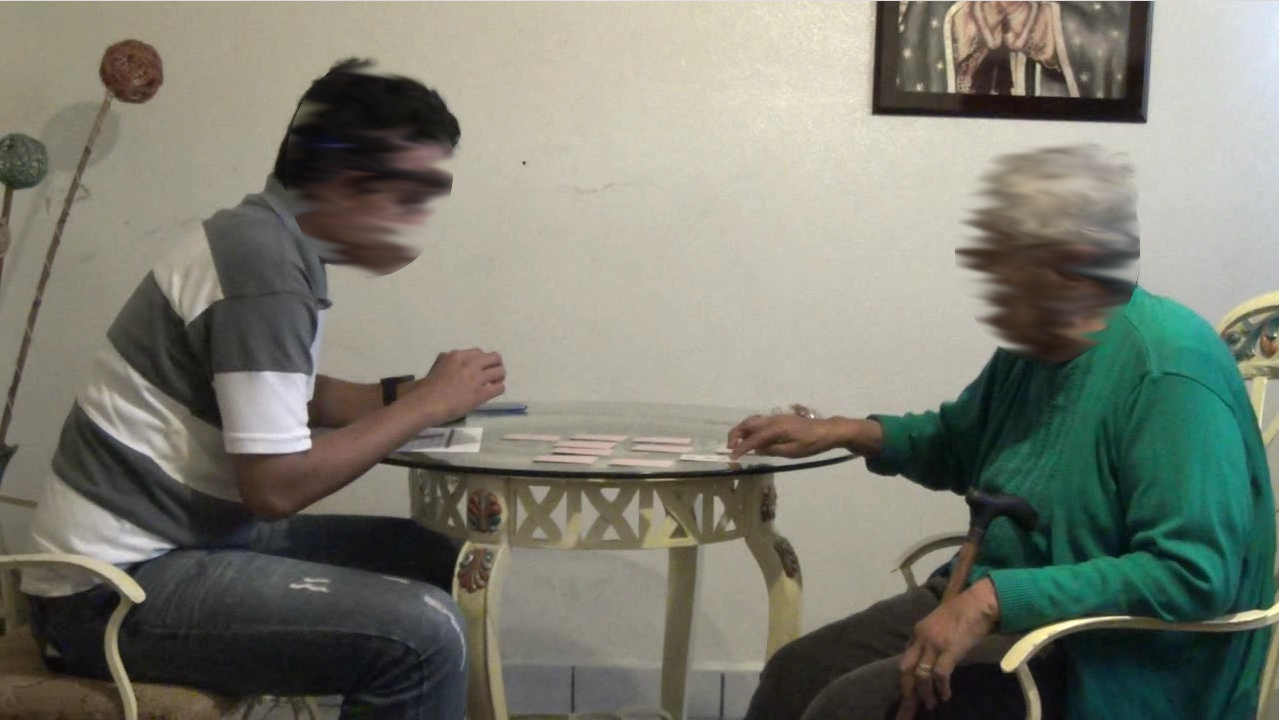
\includegraphics[width=160mm,height=80mm]{./Figures/img_memorama.png}}
	\subfigure[]{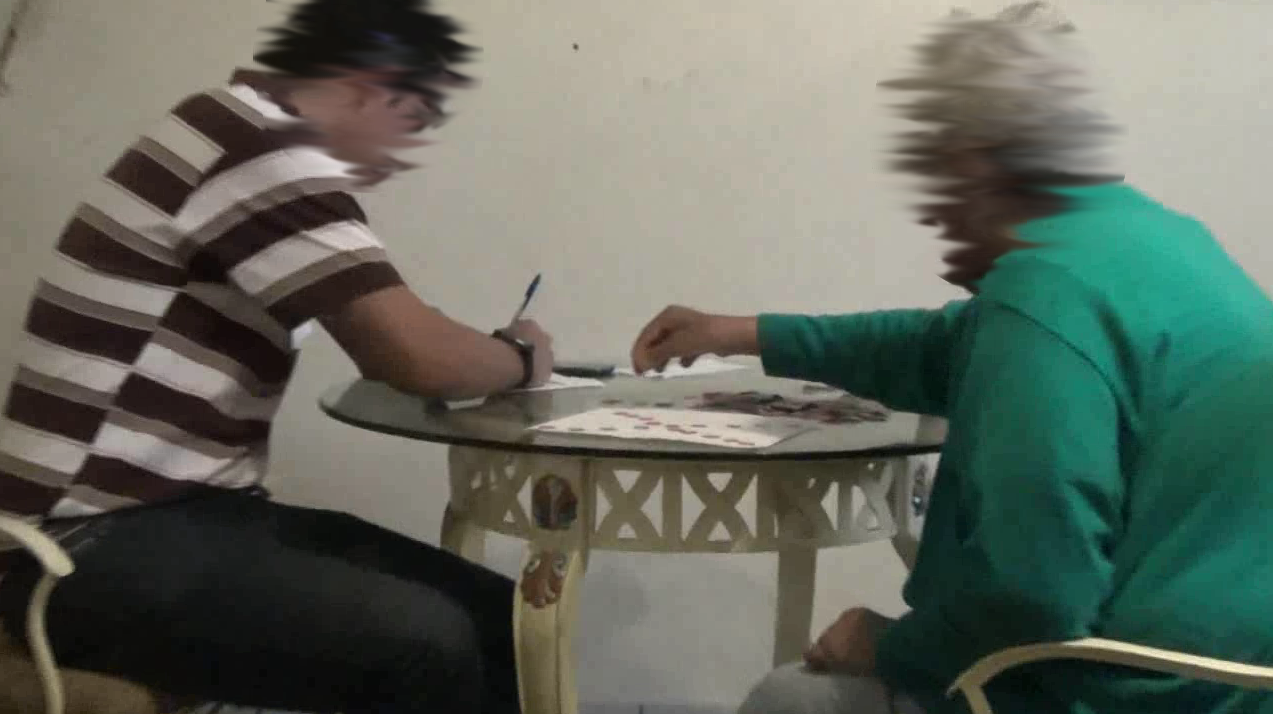
\includegraphics[width=160mm,height=80mm]{./Figures/img_fichas.png}}
	\caption{a) Participante 7 durante una terapia de memorama. b) Participante 7 durante una terapia de separaci\'on de objetos.}\label{fig:imgtherapies}

\end{figure}
%\begin{itemize}
%	\item Atado de agujetas.
%%	\item Separaci\'on de objetos.
%	\item Memorama.
%	\item Clasificaci\'on de im\'agenes.
%	\item Formaci\'on de palabras with syllables.
%	\item Sentences with words.
%	\item Formaci\'on de palabras.
%	\item Cruzigrama.
%\end{itemize}

Toda la intervenci\'on dur\'o 15 d\'ias, cada prueba de los participantes dur\'o alrededor de 30 minutos. Cada d\'ia dos participantes asistieron al sitio.

Cada participante asisiti\'o a tres sesiones. Por cada sesi\'on, una o dos tareas fueron realizadas, con varias iteraciones en cada tarea. Ninguna de las terapias fueron repetidas por los participantes. Adem\'as, ninguno de los participantes asisti\'o con el mismo compa\~nero mas de una vez. Se dividi\'o el estudio de usuario en tres semanas. Cada sujeto particip\'o una vez cada semana. Se entren\'o al adulto mayor para actuar con diferentes comportamientos diruptivos de distinto nivel de intensidad. En la primer semana, ella actu\'o en niveles de 0 a 2 (Ver tabla ~\ref{table:anxilevels}). En la segunda y tercer semana, actu\'o niveles de 0 a 3. En la \'ultima, se les ense\~n\'o a los participantes a usar estrategias de afrontamiento.
\section{Configuraci\'on}\label{secc:setup}
	Se acondicion\'o un cuarto dentro de una casa real para hacerlo parecer como si fuera la sala de una persona con demencia. La utiler\'ia incluy\'o: Muebles viejos, baja iluminaci\'on, fotograf\'ias viejas, pistas de papel sobre el lavamanos, entre otras. Una mesa de madera fue usada para instalar el equipo: una Macbook, una videoc\'amara, y un tel\'efono inteligente para monitorear el estudio de usuario.
\begin{figure}[h!]
        \centering
        \subfigure[]{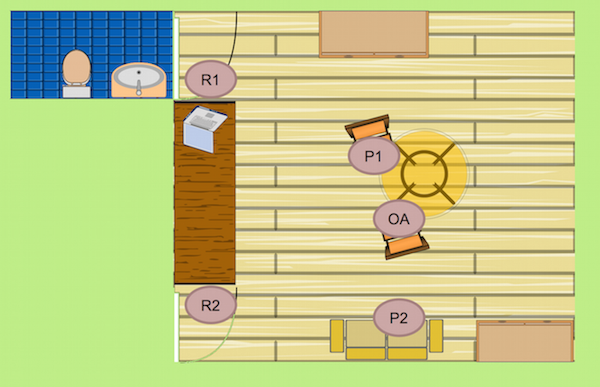
\includegraphics[width=160mm,height=80mm]{./Figures/img_exp_setup}}
	\caption{Escenario del estudio de usuario. Las actividades fueron realizadas sobre una mesa, con el actor de un adulto mayor con demencia (OA) y el participante (P1) sentados frente a frente. El segundo participante (P2) observaba sobre el sof\'a, mientras que dos investigadores (R1,R2) monitoreaban la sesi\'on desde una mesa cercana.} \label{fig:img_exp_setup}
\end{figure}

\begin{figure}[h!]
        \centering
        \subfigure[]{\includegraphics[width=160mm]{./Figures/img_exp_pics}}
	\caption{Fotograf\'ias del escenario real.} \label{fig:img_exp_pics}
\end{figure}
Dos investigadores permanecieron parados al lado de la mesa de madera para operar el equipo y tomar notas (Ver figuras ~\ref{fig:img_exp_setup} y ~\ref{fig:img_exp_pics}). La persona que actuaba como si tuviera demencia y el cuidador permanecieron sentados frente a frente en una mesa circular. Se les pidi\'o a los participantes usar el cuarto de ba\~no para vestir la banda Zephyr debido a que se pone debajo de la ropa, en contacto con la piel. Un segundo participante se sent\'o sobre el sof\'a y le pedimos que observara la sesi\'on. Este participante tambi\'en fue monitorizado por medio de \'unicamente una pulsera Empatica E3.


\subsection{Obtenci\'on de datos}\label{secc:datagathering}
Se desarrollaron dos aplicaciones separadas para el sensor Empatica E3 y el banda Zephyr HxM. Para el primer dispositivo se desarroll\'o la aplicaci\'on ``Care Me Too'' para android (ver figura ~\ref{fig:caremetoo}) la cual se conecta al dispositivo E3 v\'ia Bluetooth Low Energy (BLE), muestra los datos en tiempo real y los guarda en formato .csv. Esta aplicaci\'on tambi\'en puede ayudar a etiquetar eventos con ayuda del usuario.


\begin{figure}[h]
        \centering
        \subfigure[]{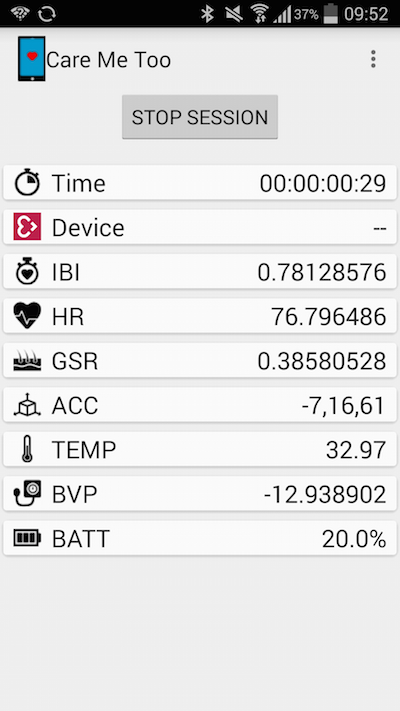
\includegraphics[height=80mm]{./Figures/img_caremetoo}}
        \caption{La aplicaci\'on Care Me Too mostrando se\~nales fisiol\'ogicas siendo grabadas.}\label{fig:caremetoo}
\end{figure}

Para obtener datos del ritmo card\'iaco de la banda Zephyr HxM se utiliz\'o el programa de l\'inea de comandos ``anxiLogger''\footnote{https://github.com/panzerfausten/anxiLogger} desarrollado por el autor para un estudio anterior \citep{Miranda}. El archivo csv de salida fue agregado a los datos de sesi\'on para sincronizar los tiempos a trav\'es de una librer\'ia llamada ``maxiProcesser''\footnote{https://github.com/panzerfausten/maxiProcesser}
	Para la banda Muse se us\'o la aplicaci\'on de escritorio ``Muse lab''. Los datos obtenidos en formato .muse fueron exportados a .csv para analizarlos posteriormente.

	Se us\'o una laptop Macbook en el sitio para conectar las bandas Muse y Zephyr y un tel\'efono inteligente Samsung Galaxy S4 para colectar datos. Los datos del participante observador fueron obtenidos a trav\'es de una segunda pulsera Empatica E3 en modo de grabaci\'on. Este modo no requiere de una conexi\'on bluetooth.


\section{Obtenci\'on de l\'inea base}\label{secc:dataanalysis}
Un reto del estudio de usuario fue identificar cuando los participantes sent\'ian ansiedad. Para lograrlo, se utilizaron tres diferentes t\'ecnicas: An\'alisis de video, observaci\'on directa y autoreportado. La figura ~\ref{fig:labeling} muestra el proceso unificado de etiquetado. A continuaci\'on se explica el procesamiento de cada fuente.

\begin{figure}[h]
        \centering
        \subfigure[]{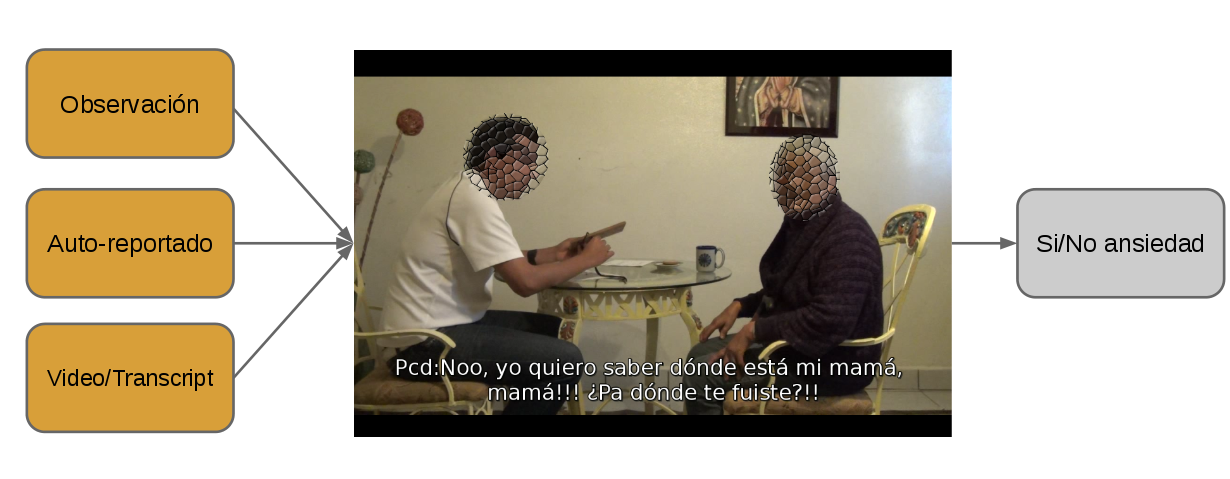
\includegraphics[height=100mm,width=160mm,keepaspectratio]{./Figures/img_labeling}}
	\caption{Proceso de etiquetado a partir de tres diferentes fuentes.}\label{fig:labeling}
\end{figure}
	\subsection{Procesamiento de video}\label{secc:videoprocesing}

	Todos los videos fueron transcritos utilizando el programa F5 transkript para Mac OS X. Con el archivo de transcripci\'on, se generaron subt\'itulos para facilitar el an\'alisis. Luego, se etiquet\'o linea por linea el comportamiento del actor de un adulto mayor con demencia. Cada linea fue clasificada en una de los tres posibles niveles que cumplieran con un criterio (ver tabla ~\ref{table:anxilevels}).  La figura ~\ref{fig:f5transcript} muestra una porci\'on de la transcripci\'on de la sesi\'on de un participante
\begin{figure}[h!]
        \centering
        \subfigure[]{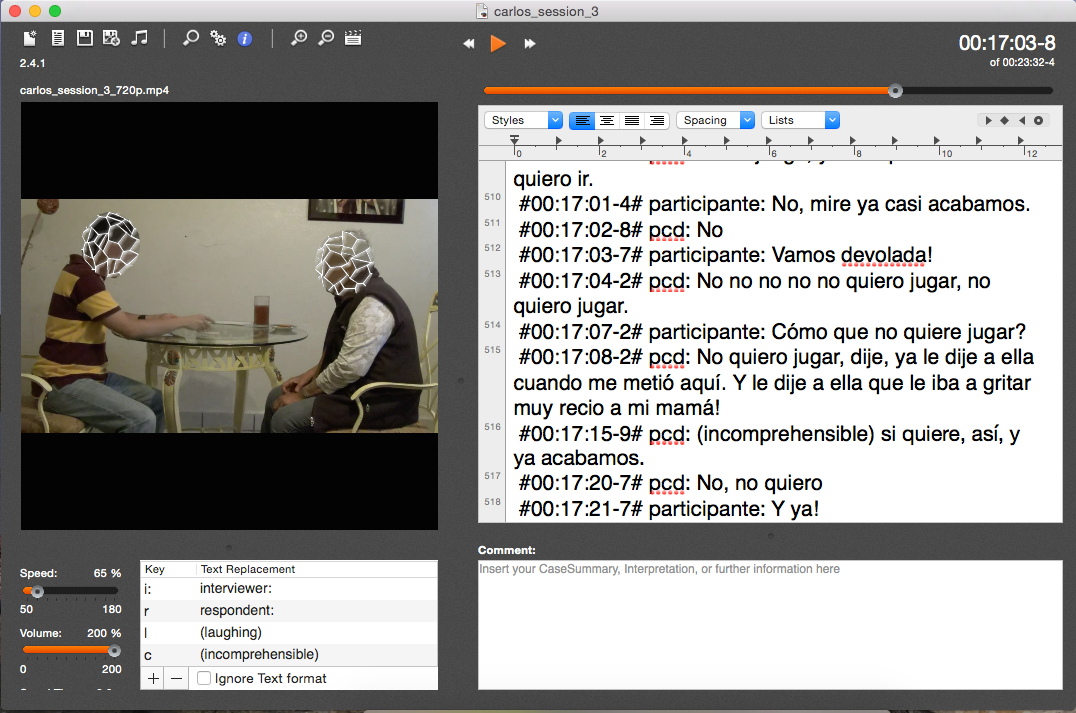
\includegraphics[height=10cm,keepaspectratio]{./Figures/img_experiment.png}}
        \caption{Transcripci\'on correspondiente a una sesi\'on completa de un participante}\label{fig:f5transcript}
\end{figure}

%La figura ~\ref{fig:imgsegment} ejemplifica un segmento extra\'ido. En el siguiente cap\'itulo se explica como se clasificaron los datos y los resultados de la detecci\'on.

%\begin{figure}[h]
%        \centering
%        \subfigure[]{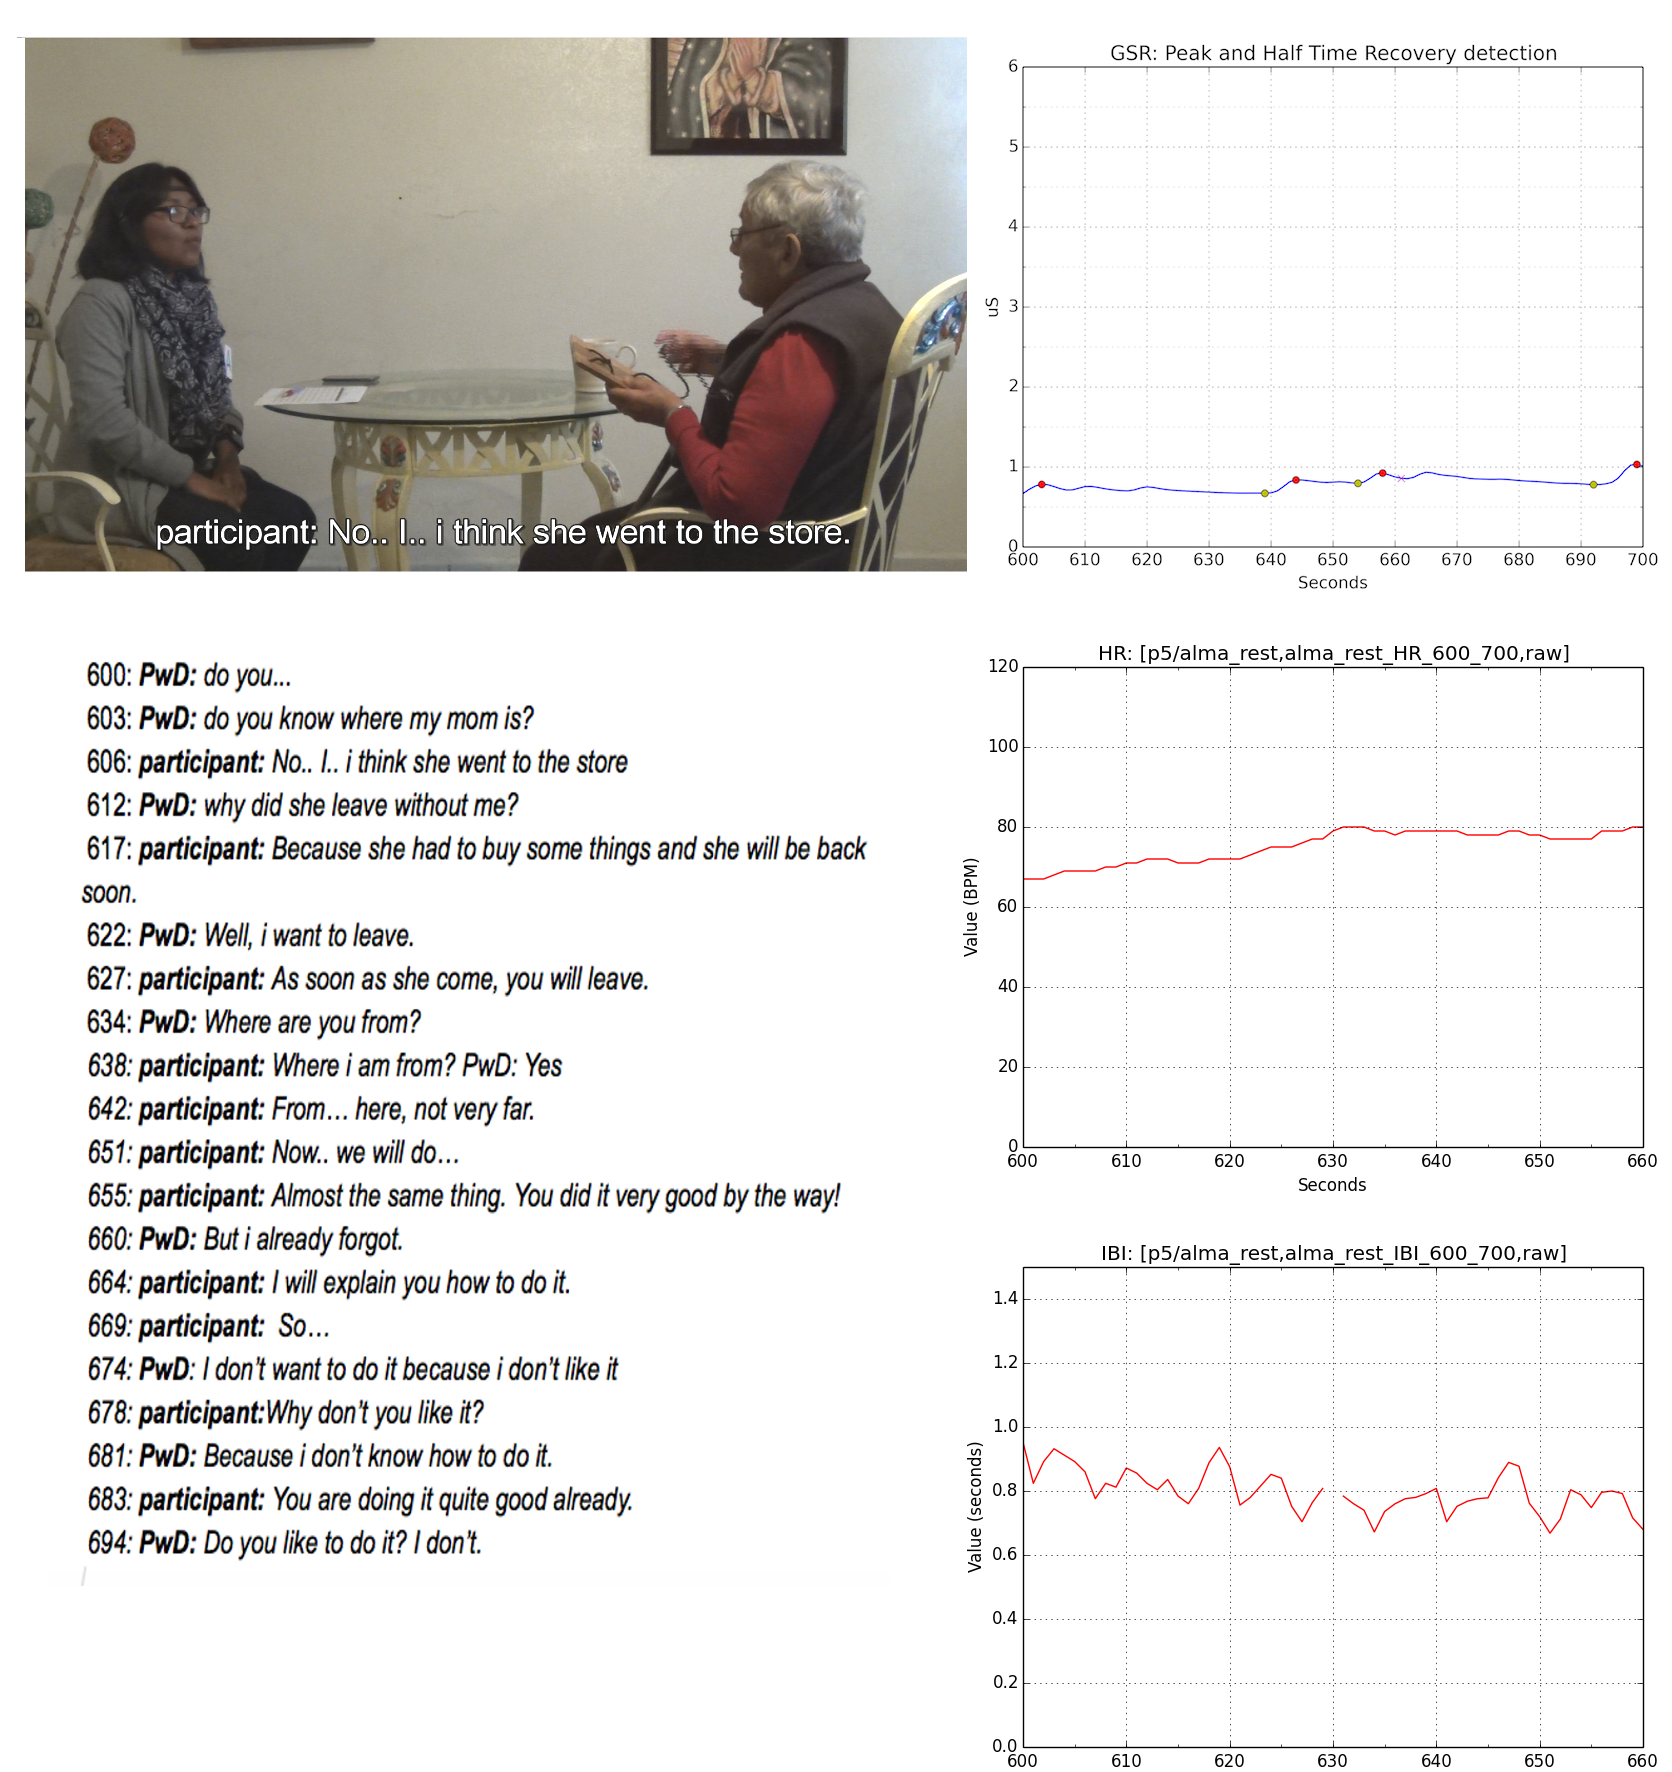
\includegraphics[height=18cm,keepaspectratio]{./Figures/img_segment.png}}
%        \caption{Transcripci\'on y se\~nales GSR, HR, e IBI correspondientes a una situaci\'on estresante}\label{fig:imgsegment}
%\end{figure}

	\subsection{Observaci\'on}
	Dos investigadores realizaron observaci\'on en el sitio, tomando nota del tiempo, nivel del comportamiento del actor de un adulto mayor con demencia, y una descripci\'on del evento. Esta descripci\'on fue escrita en base a lo que el participante y/o la aPcD dijo o hizo en el momento. El nivel de comportamiento fue codificado en base a la tabla ~\ref{table:anxilevels}. Esta codif\'ificaci\'on no es un instrumento de medici\'on de ansiedad, sino una clasificaci\'on que describe el comportamiento del aPcD y ayuda como informaci\'on extra para pasos posteriores. La secci\'on ~\ref{secc:unificacion} muestra como esta informaci\'on es unida con otras fuentes. Un evento etiquetado como ``0'' corresponde a cuando la aPcD se encuentra realizando la tarea como se le pidi\'o. En esta situaci\'on el cuidador puede estar totalmente relajado o bien ligeramente estresado. En un evento con la etiqueta ``1'' la aPcD se encuentra en un estado renuente diciendo cosas como ``No me gusta esta tarea'' o ``Hazlo tu, yo no quiero''. La aPcD podr\'ia estar realizando la tarea con bajo rendimiento o podr\'ia no prestar atenci\'on del todo. En un nivel ``2'', la aPcD realiza situaciones no esperadas como preguntar al participante por su madre o cualquier otra pregunta que lo ponga inc\'omodo. La atenci\'on hacia la tarea puede ser muy baja. En el nivel ``3'', la aPcD realiza acciones como tratar de golpear al participante, levantarse de la silla y querer salir de la habitaci\'on o gritar. La atenci\'on a la tarea suele ser nula. La figura~\ref{fig:imgobservation} ejemplifica la observaci\'on correspondiente a una sesi\'on.

	\begin{table}[h!]
		\footnotesize
		\centering
		\caption{Criterio de etiquetado de comportamiento de la aPcD.}
		\label{table:anxilevels}
		%\rotatebox{90}{
		\begin{tabular}{m{2.5cm}m{5.0cm}m{5.0cm}m{2.5cm}}
			\hline\noalign{\smallskip}

		    \textbf{Nivel} & \textbf{Criterio}                                                                                    & \textbf{Ejemplo de evento}                                                                      \\ \hline
			\\ \noalign{\smallskip}

			    0     & \pbox{12cm}{La aPcD actua de forma pasiva,\\La aPcD accede a participar,  \\El participante y la aPcD \\est\'an haciendo la tarea} &                   \pbox{12cm}{La aPcD est\'a realizando la\\ tarea como se le pidi\'o.}                       \\ 
	      1     & \pbox{12cm}{Comportamientos renuentes.,\\Reacio a participar,\\Quejandose acerca de la tarea.}                & \pbox{12cm}{ ``No me gusta este juego.'' \\ ``Esto es muy dif\'icil.'' \\``Hazlo tu.'' }             \\ 
	      2     & \pbox{12cm}{Murmureo,\\Hablando cosas sin sentido,  \\Comportamientos impredecibles}                                      & \pbox{5cm}{``?`Donde est\'a mi mam\'a?''\\``Qui\'en eres?''}                                          \\ 
	      3     & \pbox{12cm}{Gritos.\\Amenazas al particpante,\\Paranoia,  \\Urgencia de irse.}                          & \pbox{12cm}{``MAM\'A, DONDE EST\'AS!!??''\\``YA QUIERO IRME!''  \\``QUIEN ERES? D\'EJAME IR!'' } \\ 
		\end{tabular}
		%}
	\end{table}
\begin{figure}[h]
        \centering
        \subfigure[]{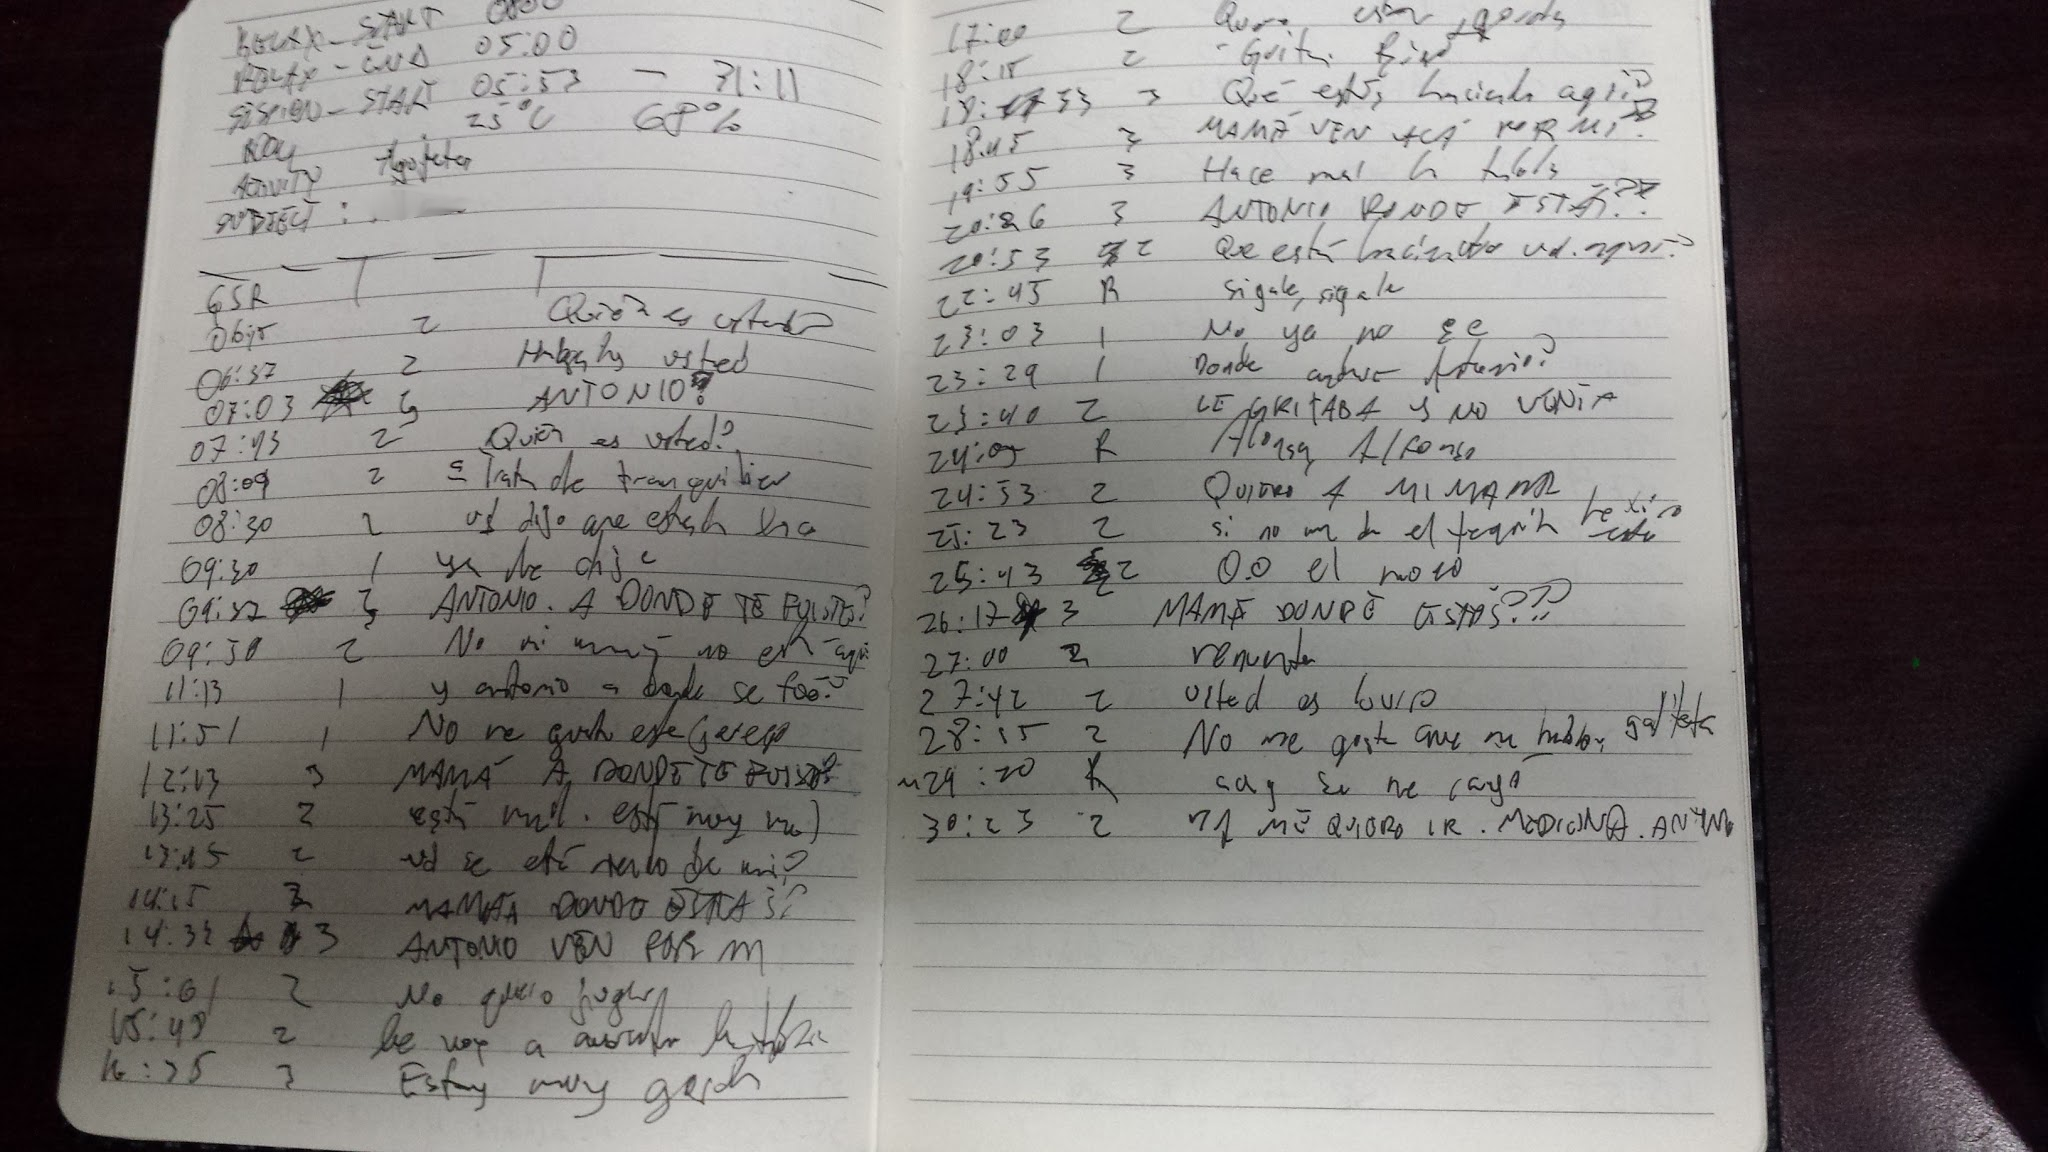
\includegraphics[height=200mm,width=160mm,keepaspectratio]{./Figures/img_observation.png}}
        \caption{Libreta de observaci\'on. Se anot\'o el tiempo con respecto al inicio de la sesi\'on, el nivel de evento de la aPcD percibido y una porci\'on del dialogo como referencia. Otros datos como la temperatura y humedad relativa del cuarto fueron anotados.}\label{fig:imgobservation}
\end{figure}
	\subsection{Autoreportado}
	Se les entreg\'o a los participantes un formulario en papel para indicar su nivel de ansiedad mientras desarrollaban la tarea. La escala del nivel de ansiedad fue tomada de la escala de ansiedad subjetiva autocalificada explicada en el ~\ref{capit:cap2}. Se les explic\'o a los participantes durante la sesi\'on de entrenamiento como utilizar el formulario de auto reportado. Sin embargo, algunos de ellos encontraron dif\'icil de contestarlo adecuadamente, principalmente porque estaban muy ocupados con la terapia. La figura ~\ref{fig:imggtlabel} ejemplifica el auto reportado de un participante que contest\'o correctamente el formulario.
	\begin{figure}[h!]
		\centering
		\subfigure[]{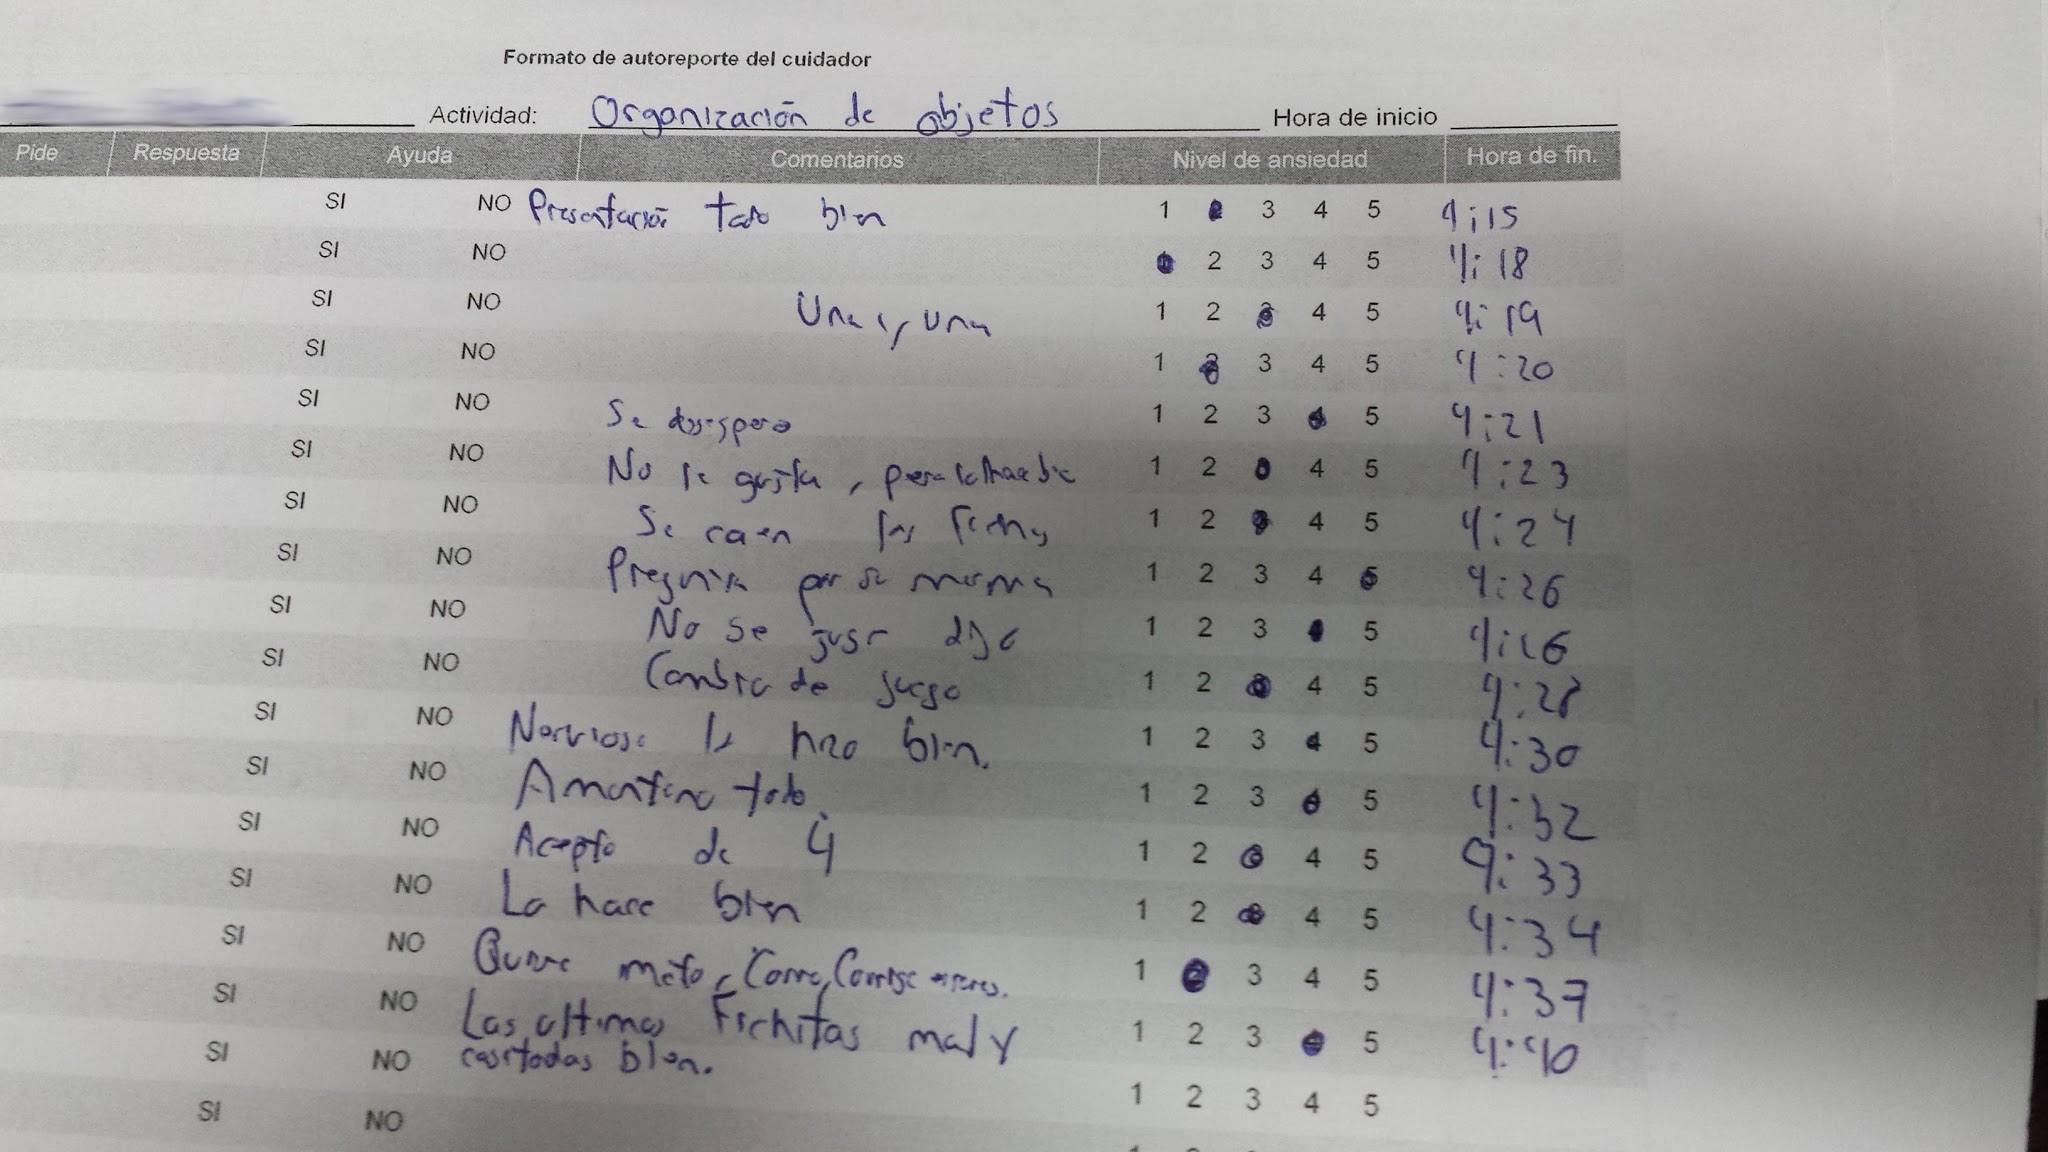
\includegraphics[height=200mm,width=160mm,keepaspectratio]{./Figures/img_sr.png}}
		\caption{Formato de auto reportado de una sesi\'on completa de un participante}\label{fig:imggtlabel}
	\end{figure}

	\subsection{Unificaci\'on de l\'inea base}\label{secc:unificacion}
	Por \'ultimo, se gener\'o un formato con los datos de transcripci\'on, nivel del evento del actor de un adulto mayor con demencia y auto reportado. Al mismo tiempo, se observ\'o el video para obtener rasgos de ansiedad como cambios en la tonalidad de voz, desv\'io de mirada, o movimientos del participante. Con esta informaci\'on, se etiquet\'o cada 30 segundos si exist\'ia ansiedad o no. Se anot\'o con el n\'umero ``1'' cuando claramente el participante experimentaba ansiedad y con un ``0'' si claramente no. Si el segmento era muy ambiguo (p. ej. El participante se ve ansioso en el video pero el nivel del auto reportado y el evento de la PcD eran bajos) se etiquet\'o con el n\'umero ``-1''. La figura ~\ref{fig:imggtlabel} ejemplifica un segmento codificado.
	\begin{figure}[h!]
		\centering
		\subfigure[]{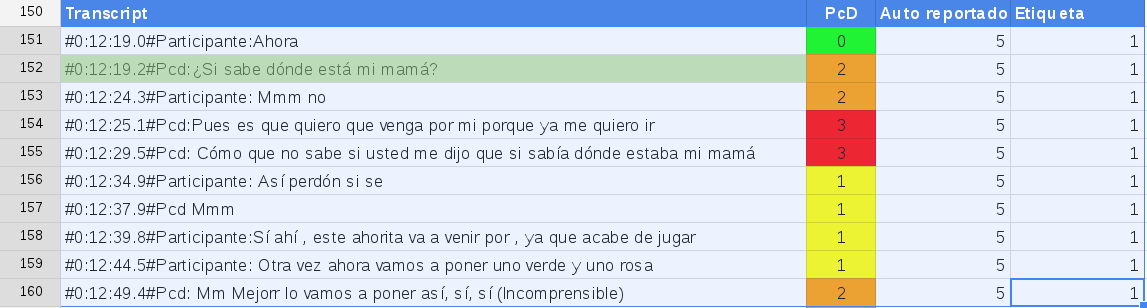
\includegraphics[height=200mm,width=160mm,keepaspectratio]{./Figures/img_gtlabel.png}}
		\caption{Segmento codificado como ansiedad. El nivel de auto reportado es alto y existen valores altos en el comportamiento de la aPcD. }\label{fig:imggtlabel}
	\end{figure}
\section{Preprocesamiento de GSR}\label{secc:gsrpreprocessing}
Se desarroll\'o una librer\'ia en python para procesar todos los datos fisiol\'ogicos, incluyendo funciones para exportar, extraer caracter\'isticas, sincronizaci\'on de tiempos, y graficado de datos de ansiedad de todos los dispositivos. La librer\'ia tambi\'en puede graficar atributos de la se\~nal GSR (picos, tiempos de recuperaci\'on medios, amplitudes, etc.) y guardar los datos en formato .csv y .json.

Se inici\'o remuestreando los datos de GSR de 4.0 Hz a 1.0 Hz calculando el valor promedio de todos los datos que cayeran en una ventana deslizante de 1 segundo. Esto se hizo debido a que se esperaba que los periodos de ansiedad duraran segundos. Luego, se aplic\'o un filtro gausiano para suavizar la se\~nal y el ruido. Finalmente, se us\'o un m\'etodo de la librer\'ia scipy de python para detectar picos y se filtraron todos los picos con amplitud mas grande que un umbral ($t \geqslant 0.04$ para datos no normalizados y $t \geqslant 0.01$ para datos normalizados en base a experimentaci\'on e inspecci\'on visual) con la finalidad de evitar variaciones dadas por el sensor o muy peque\~nas para tener una utilidad. Tambi\'en se calcul\'o el ``Tiempo de media recuperaci\'on'' de la se\~nal. Esto es, el punto donde la se\~nal decae al valor exacto de la mitad del pico.
\section{Preprocesamiento de HR e IBI}\label{secc:hribipreprocessing}
No fue necesario remuestrear los datos de HR e IBI debido a la naturaleza de la se\~nal. El sensor solo reporta datos cuando ocurre un latido del coraz\'on. Sin embargo, se agrup\'o en ventanas de segundos para compararlo con el resto de las se\~nales. El ruido de los datos fu\'e muy bajo y no requiri\'o pre-procesamiento adicional.
\section{Extracci\'on de caracter\'isticas}
Una vez segmentadas y etiquetadas las sesiones, se tomaron varias caracter\'isticas por cada tipo de se\~nal. Estas caracter\'isticas generalizan al evento completo. La tabla ~\ref{tab:features} describe dichas caracter\'isticas.

	\begin{table}[t]
		\footnotesize
		\centering
        	\caption{Caracter\'isticas usadas como entrada para el clasificador de SVM}
 	       \label{tab:features}

		%\rotatebox{90}{
		\begin{tabular}{m{2.5cm}m{5.0cm}m{5.0cm}m{2.5cm}}
			\hline\noalign{\smallskip}

                \textbf{Se\~nal} & \textbf{Caracter\'istica} & \textbf{Descripci\'on} & \textbf{Unidad} \\
		\hline
			\\ \noalign{\smallskip}
                GSR   & \pbox{12cm}{\textit{Amplitud de los picos}}                & \pbox{12cm}{Distancias promedio \\desde el punto de crecimiento\\ hacia el pico}             & \pbox{12cm}{$\mu S$}        \\
                GSR   & \pbox{12cm}{\textit{Amplitud m\'axima de los picos}}                & \pbox{12cm}{Amplitud mas grande \\ de los picos}             & \pbox{12cm}{$\mu S$}        \\
                GSR   & \pbox{12cm}{\textit{Amplitud m\'inima de los picos}}                & \pbox{12cm}{Amplitud mas chica \\ de los picos}             & \pbox{12cm}{$\mu S$}        \\
                GSR   & \pbox{12cm}{\textit{Varianza de los picos}}                & \pbox{12cm}{Varianza total de todos\\ los picos}             & \pbox{12cm}{$\mu S$}        \\
			GSR   & \pbox{12cm}{\textit{Tiempo promedio de} \\\textit{media recuperaci\'on de los picos}}                & \pbox{12cm}{Varianza total de todos\\ los picos}             & \pbox{12cm}{$\mu S$}        \\
                IBI   &\textit{M\'inimo}                & Valor m\'inimo del segmento            &Segundos       \\
                IBI   &\textit{M\'aximo}                & Valor m\'aximo del segmento            &Segundos       \\
                IBI   &\textit{Promedio}                & Valor promedio del segmento            &Segundos       \\
                IBI   &\textit{Desviaci\'on estandar}                &  \pbox{12cm}{Desviaci\'on estandar de todos\\ los datos del segmento}            &Segundos        \\


        \end{tabular}
\end{table}
%TODO:UPDATE THIS 
%Para este trabajo, se tuvo un total de 51 segmentos del nivel 0, 177 del nivel 1, 145 del nivel 2 y 106 del nivel 3. Los datos corresponden a 5 del total de 10 de participantes. Utilizando 15 sesiones. No se procesaron todas las sesiones en su totalidad, debido al extenso tiempo necesario para transcribir los videos. Todos los segmentos fueron luego codificados en forma de vectores descriptores. Estos vectores fueron guardados en formato .csv, con la primera columna correspondiente a la etiqueta de nivel de ansiedad.
%\section{Sincronizaci\'on de datos}
%	Agregar 
\section{Conclusi\'on}
El dise\~no de este estudio de usuario permite capturar datos de actores en un escenario concreto de cuidadores de personas con demencia que simulan condiciones cercanas a las reales. Esto abre la posibilidad de analizar por medio de tecnolog\'ia los efectos de ansiedad en los cuidadores.

En la siguiente secci\'on se utiliza una t\'ecnica de aprendizaje de m\'aquina para clasificar los eventos de ansiedad. Se explican las diferentes pruebas realizadas, y los resultados generales de este estudio de usuario.
\newpage
%%=====================================================

} }%
%BeginExpansion
\chapter{Dise\~no de un estudio de usuario para inducir ansiedad en cuidadores de personas con demencia}\label{capit:cap3}
\vspace{-2.0325ex}%
\noindent
\rule{\textwidth}{0.5pt}
\vspace{-5.5ex}% 
\newcommand{\pushline}{\Indp}% Indent puede ir o no :p
\section{Introducci\'on}\label{secc:introduction}

Como vimos en el cap\'itulo 2, la mayor\'ia de los estudios logran inducir ansiedad o estr\'es por medio de situaciones controladas dentro del laboratorio. Sin embargo, generar ansiedad en cuidadores informales es mucho mas dif\'icil. El escenario de un laboratorio no coincide con el entorno en el que una persona con demencia se desarrolla, por lo que los comportamientos impredecibles no ser\'ian congruentes con dicho ambiente. Adem\'as, exponer a personas sin experiencia ante una persona con demencia que tiene necesidades reales resultar\'ia riesgoso para ambos individuos. Por otra parte, realizar una intervenci\'on totalmente natural a\~nade un grado de dificultad al estudio, resultando en ruido en los datos recolectados (p. ej. la se\~nal de ritmo card\'iaco podr\'ia ser alta no por una situaci\'on de ansiedad, sino por una actividad f\'isica, m\'ultiples distracciones o responsabilidades al mismo tiempo para el cuidador) haciendo d\'ificil de analizarlos.

En este cap\'itulo se explica el uso de una t\'ecnica llamada ``Naturalistic Enactment (NE)'' \citep{Castro11} dentro de un estudio de usuario para capturar datos de ansiedad en cuidadores de personas con demencia.


\section{Un estudio de usuario para inducir ansiedad en cuidadores informales}\label{secc:experiment}
Se dise\~n\'o un estudio de usuario para inducir ansiedad en cuidadores informales bajo situaciones simuladas y parecidas a la realidad. Para lograr esto, se utiliz\'o la t\'ecnica de NE. NE fue propuesta originalmente para evaluar tecnolog\'ias m\'edicas ubicuas, donde el tener una validez ambiental e interacc\'on directa del usuario es importante, y donde sin embargo, utilizar pacientes reales puede ser peligroso \citep{Castro11}. NE consiste del desarrollo de tareas reales (p. ej. la exposici\'on a situaciones y tareas en situaciones naturales) para simular la experiencia del usuario bajo condiciones normales, y por lo tanto encontrar problemas y comportamientos que pudieran de otra manera haber sido dif\'iciles de capturar. NE representa una ventaja ante otros m\'etodos de evaluaci\'on gracias a su alta fidelidad, mediano riesgo y alta involucramiento del usuario (Ver figura ~\ref{fig:evalmethods}).

\begin{figure}[h]
        \centering
        \subfigure[]{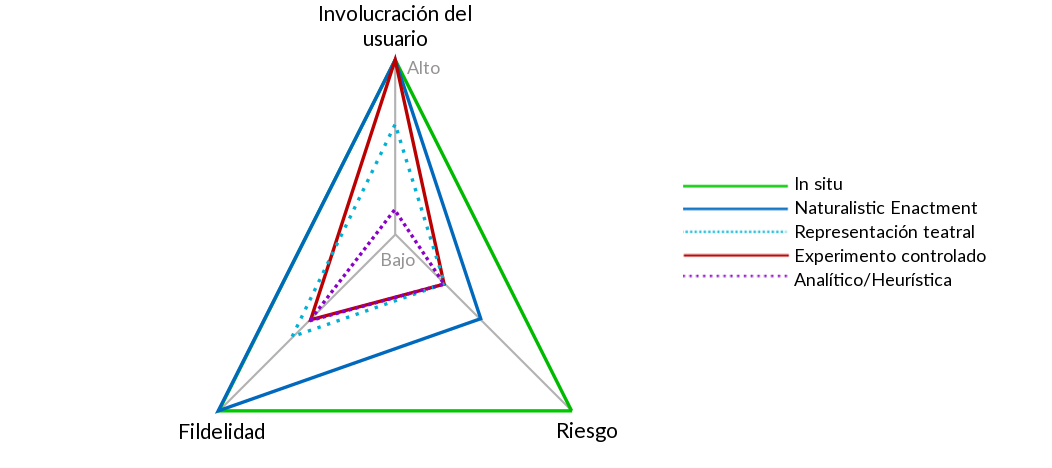
\includegraphics[width=160mm]{./Figures/img_evalmethods}}
	\caption{M\'etodos de evaluaci\'on clasificados de acuerdo a la involucramiento del usuario, fidelidad y riesgo \protect\citep{Castro11} }\label{fig:evalmethods}
\end{figure}


Para poder exponer a los sujetos a una situaci\'on de cuidador, estresante y realista, bajo condiciones controladas; se formul\'o un ejercicio que consisti\'o de una situaci\'on de terapia real con una persona actuando como si tuviera demencia. Un adulto mayor de 75 a\~nos actu\'o como si sufriera de demencia. Una especialista en intervenciones con adultos mayores con demencia le entren\'o con los comportamientos t\'ipicos de demencia moderada como: murmureo, gritos, vagabundeo, preguntas repetitivas, entre otras. Ella ya estaba familiarazada con estos comportamientos por conocidos que sufrieron de demencia. En cambio, se les dijo que se evaluaba su rendimiento como cuidadores basados en el entrenamiento inicial que se les di\'o. Para fines pr\'acticos de esta tesis, se referir\'a al adulto mayor como actor de un adulto mayor con demencia (aPcD).

Se les pidi\'o firmar un documento de no divulgaci\'on (Ver Ap\'endice~\ref{aped:cartanodiv}) para evitar que los participantes hablaran entre ellos acerca del estudio de usuario, de los comportamientos del adulto mayor o cualquier otra t\'ecnica acerca de como manejar el comportamiento del adulto mayor, durante el tiempo en que el estudio de usuario durara.

\subsection{Participantes}\label{secc:subjects}
Los sujetos fueron reclutados a trav\'es de la lista de correo de CICESE (3 personas), por el departamento de ciencias de la computaci\'on (5 personas) y dos personas externas a la instituci\'on. Se les otorg\'o un premio de compensaci\'on de 100.00 MXN en dinero electr\'onico para el cine. Se les pidi\'o a los participantes asisitr a 3 sesiones (una por cada semana), cada sesi\'on dur\'o al rededor de 30 minutos. Para simular el escenario de una persona que reci\'en toma un papel de cuidador se excluyeron a personas que fueran cuidadores que fueran cuidadores en el momento. Se incluyeron a personas que tuvieran experiencia previa como cuidadores informales para realizar comparaciones futuras (ver Trabajo a futuro). Se les dijo que estar\'ian trabajando con una persona que realmente ten\'ia demencia. Tambi\'en, se les ocult\'o la verdadera raz\'on del estudio. Se obtuvo consentimiento firmado de todos los sujetos (Ver Ap\'endice ~\ref{aped:cartainfo})

Todos los sujetos participaron en una sesi\'on de entrenamiento, en donde una especialista en intervenciones con adultos mayores con demencia les explic\'o las actividades a realizar en las terapias que hicieron con el adulto mayor.
Participaron 10 estudiantes (5 hombres y 5 Mujeres) con un promedio de 24.5 a\~nos de edad ($\sigma=1.059$). La tabla \ref{table:kysymys} muestra los datos demogr\'aficos de los participantes.
\begin{table}
	\footnotesize
	\centering
	\caption{Participantes en el estudio}
	\label{table:kysymys}
	%\rotatebox{90}{
	\begin{tabular}{m{0.2cm}m{2.5cm}m{2.5cm}m{2.5cm}m{2.5cm}}
		\hline\noalign{\smallskip}
		 & \textbf{Sujeto} & \textbf{G\'enero} & \textbf{Edad} & \textbf{Experiencia de cuidador}
		\\ \noalign{\smallskip}
		\hline
		\noalign{\smallskip}
		&S1& Masculino & 24 & No   \\ 
		&S2& Masculino &  25&  No  \\ 
		&S3& Femenino & 24 & No   \\ 
		&S4& Femenino & 26 & No  \\ 
		&S5& Femenino & 24 & No   \\ 
		&S6& Masculino & 26 &  No  \\ 
		&S7& Masculino & 23 &  No \\ 
		&S8& Masculino & 25 &  Si  \\ 
		&S9& Femenino & 26 & No   \\ 
	  	&S10& Femenino & 24 & Si  \\ 
		\hline
	\end{tabular}
	%}
\end{table}
\section{Procedimiento}\label{secc:methods}
El desarrollo del estudio de usuario se dividi\'o en diferentes actividades. A continuaci\'on se explican a detalle cada una de ellas.
\subsection{Entrenamiento}\label{secc:training}
	Todos los sujetos participaron en una sesi\'on de entrenamiento para familiarizarse con las terapias cognitivas que har\'ian con el adulto mayor. La sesi\'on de entrenamiento dur\'o aproximadamente 90 minutos. Todos los participantes practicaron las terapias y tuvieron oportunidad de hacer preguntas. No se les di\'o ninguna estrategia de afrontamiento acerca de como lidiar con los comportamientos del adulto mayor. Se les dijo a los participantes que el adulto mayor ten\'ia declive cognitivo ligero y que podr\'ia mostrar algunos problemas de comportamiento como olvidar instrucciones recientes, apat\'ia y renuencia de completar las tareas, entre otras. Se les dijo que las tareas no ten\'ian que ser completadas si el adulto mayor no estaba cooperando, pero que deber\'ian intentar completar la terap\'ia.

\subsection{Tareas de terapias}\label{secc:therapytasks}
Antes de iniciar la tarea, equipamos a los participantes con una banda de pecho Zephyr Hxm para monitorear su ritmo card\'iaco, una pulsera Empatica E3 para obtener GSR y temperatura corporal y una banda cerebral Muse para obtener datos de EEG. Todas las sesiones fueron videograbadas para analizarlas posteriormente.

Durante cinco minutos y ya equipados con los dispositivos, se les pidi\'o a los participantes relajarase por medio de respiraci\'on profunda y con los ojos cerrados para obtener una l\'inea base de datos fisiol\'ogicos. S\'olo una persona necesit\'o mas de 5 minutos debido a que tuvo problemas para relajarse.

Se les pidi\'o a los participantes que guiaran al adulto mayor a trav\'es de una sesi\'on de terapia que involucr\'o una de las 7 posibles tareas que fueron explicadas durante la sesi\'on de entrenamiento. La tabla ~\ref{table:therapies} presenta las tareas realizadas por cada participante en las tres sesiones del estudio. La figura ~\ref{fig:imgtherapies} muestra dos terapias de ejemplo. Los rostros de los participantes fueron modificados para mantener su privacidad.

\begin{table}[h!]
	\footnotesize
	\centering
	\caption{Terapias realizadas con el adulto mayor por cada participante.}
	\label{table:therapies}
	%\rotatebox{90}{
	\renewcommand{\arraystretch}{1.5}
	\begin{tabular}{m{0.2cm}m{3.5cm}m{3.5cm}m{3.5cm}m{3.5cm}}
		\hline\noalign{\smallskip}
	&\textbf{Participante}&  \textbf{Terapia 1}& \textbf{Terapia 2}   & \textbf{Terapia 3}  \\ \hline
		\\ \noalign{\smallskip}
		&S1&  Atado de agujetas& Memorama & \pbox{12cm}{Clasificaci\'on\\de im\'agenes}   \\ 
  &S2&  \pbox{12cm}{Clasificaci\'on\\de im\'agenes}& Atado de agujetas & Crucigrama   \\ 
  &S3&  \pbox{12cm}{Formaci\'on de palabras}& Cruzigrama & Memorama    \\ 
  &S4&  Atado de agujetas&\pbox{12cm}{Clasificaci\'on de\\im\'agenes}& Memorama   \\ 
  &S5&  \pbox{12cm}{Clasificaci\'on\\de im\'agenes}&  Atado de agujetas & Crucigrama   \\ 
  &S6&  \pbox{12cm}{Separaci\'on de objetos}& Memorama & Atado de agujetas   \\ 
  &S7&  \pbox{12cm}{Separaci\'on de objetos}& Atado de agujetas & Crucigrama   \\ 
  &S8&  Crucigrama& Atado de agujetas &\pbox{12cm}{Clasificaci\'on\\de im\'agenes}   \\ 
  &S9&  \pbox{12cm}{Formaci\'on\\de palabras}& \pbox{12cm}{Clasificaci\'on\\de im\'agenes} & Memorama   \\ 
  &S10&  Memorama&\pbox{12cm}{Formaci\'on\\de palabras} & Atado de agujetas   \\ 
		\hline
	\end{tabular}
	%}
\end{table}

\begin{figure}[h!]
        \centering
	\subfigure[]{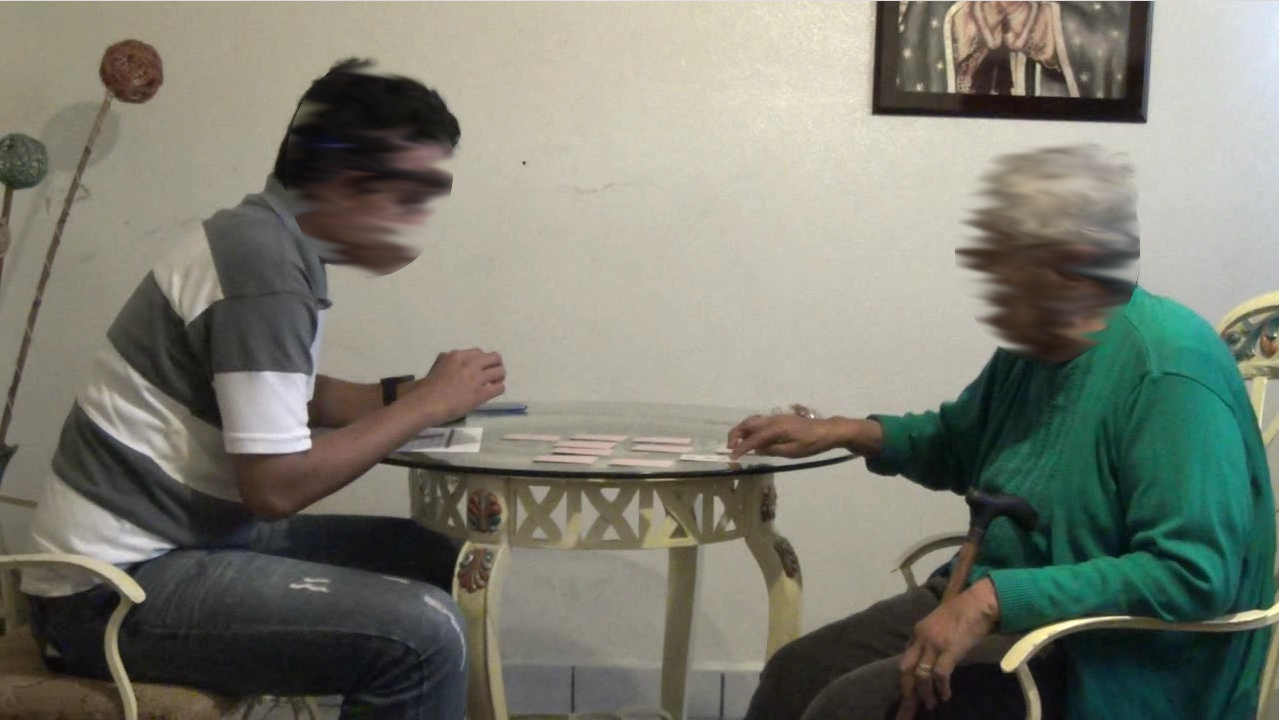
\includegraphics[width=160mm,height=80mm]{./Figures/img_memorama.png}}
	\subfigure[]{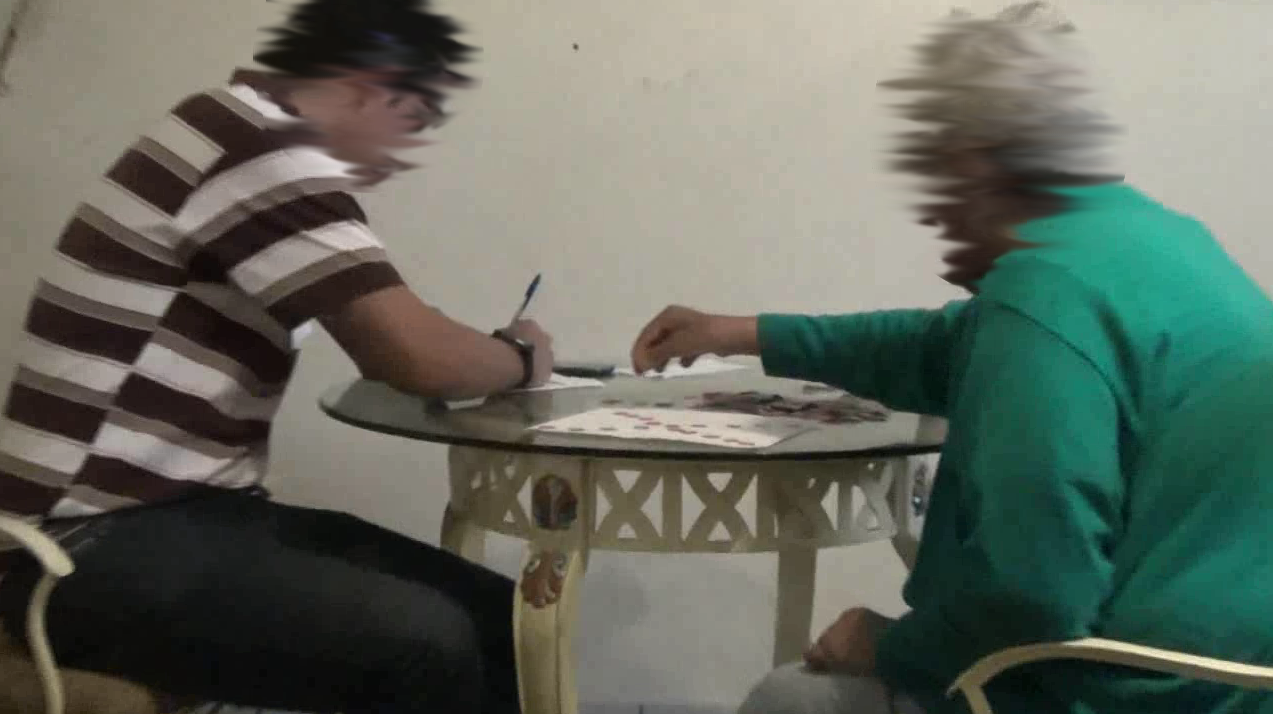
\includegraphics[width=160mm,height=80mm]{./Figures/img_fichas.png}}
	\caption{a) Participante 7 durante una terapia de memorama. b) Participante 7 durante una terapia de separaci\'on de objetos.}\label{fig:imgtherapies}

\end{figure}
%\begin{itemize}
%	\item Atado de agujetas.
%%	\item Separaci\'on de objetos.
%	\item Memorama.
%	\item Clasificaci\'on de im\'agenes.
%	\item Formaci\'on de palabras with syllables.
%	\item Sentences with words.
%	\item Formaci\'on de palabras.
%	\item Cruzigrama.
%\end{itemize}

Toda la intervenci\'on dur\'o 15 d\'ias, cada prueba de los participantes dur\'o alrededor de 30 minutos. Cada d\'ia dos participantes asistieron al sitio.

Cada participante asisiti\'o a tres sesiones. Por cada sesi\'on, una o dos tareas fueron realizadas, con varias iteraciones en cada tarea. Ninguna de las terapias fueron repetidas por los participantes. Adem\'as, ninguno de los participantes asisti\'o con el mismo compa\~nero mas de una vez. Se dividi\'o el estudio de usuario en tres semanas. Cada sujeto particip\'o una vez cada semana. Se entren\'o al adulto mayor para actuar con diferentes comportamientos diruptivos de distinto nivel de intensidad. En la primer semana, ella actu\'o en niveles de 0 a 2 (Ver tabla ~\ref{table:anxilevels}). En la segunda y tercer semana, actu\'o niveles de 0 a 3. En la \'ultima, se les ense\~n\'o a los participantes a usar estrategias de afrontamiento.
\section{Configuraci\'on}\label{secc:setup}
	Se acondicion\'o un cuarto dentro de una casa real para hacerlo parecer como si fuera la sala de una persona con demencia. La utiler\'ia incluy\'o: Muebles viejos, baja iluminaci\'on, fotograf\'ias viejas, pistas de papel sobre el lavamanos, entre otras. Una mesa de madera fue usada para instalar el equipo: una Macbook, una videoc\'amara, y un tel\'efono inteligente para monitorear el estudio de usuario.
\begin{figure}[h!]
        \centering
        \subfigure[]{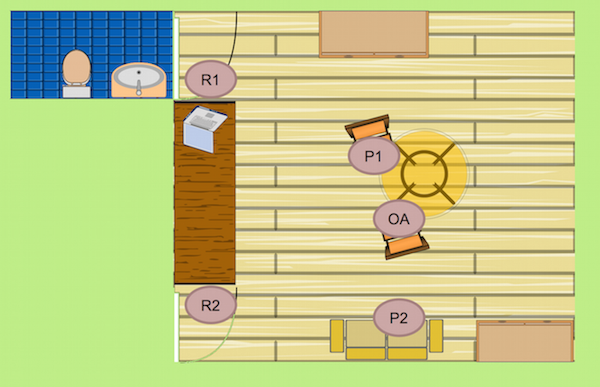
\includegraphics[width=160mm,height=80mm]{./Figures/img_exp_setup}}
	\caption{Escenario del estudio de usuario. Las actividades fueron realizadas sobre una mesa, con el actor de un adulto mayor con demencia (OA) y el participante (P1) sentados frente a frente. El segundo participante (P2) observaba sobre el sof\'a, mientras que dos investigadores (R1,R2) monitoreaban la sesi\'on desde una mesa cercana.} \label{fig:img_exp_setup}
\end{figure}

\begin{figure}[h!]
        \centering
        \subfigure[]{\includegraphics[width=160mm]{./Figures/img_exp_pics}}
	\caption{Fotograf\'ias del escenario real.} \label{fig:img_exp_pics}
\end{figure}
Dos investigadores permanecieron parados al lado de la mesa de madera para operar el equipo y tomar notas (Ver figuras ~\ref{fig:img_exp_setup} y ~\ref{fig:img_exp_pics}). La persona que actuaba como si tuviera demencia y el cuidador permanecieron sentados frente a frente en una mesa circular. Se les pidi\'o a los participantes usar el cuarto de ba\~no para vestir la banda Zephyr debido a que se pone debajo de la ropa, en contacto con la piel. Un segundo participante se sent\'o sobre el sof\'a y le pedimos que observara la sesi\'on. Este participante tambi\'en fue monitorizado por medio de \'unicamente una pulsera Empatica E3.


\subsection{Obtenci\'on de datos}\label{secc:datagathering}
Se desarrollaron dos aplicaciones separadas para el sensor Empatica E3 y el banda Zephyr HxM. Para el primer dispositivo se desarroll\'o la aplicaci\'on ``Care Me Too'' para android (ver figura ~\ref{fig:caremetoo}) la cual se conecta al dispositivo E3 v\'ia Bluetooth Low Energy (BLE), muestra los datos en tiempo real y los guarda en formato .csv. Esta aplicaci\'on tambi\'en puede ayudar a etiquetar eventos con ayuda del usuario.


\begin{figure}[h]
        \centering
        \subfigure[]{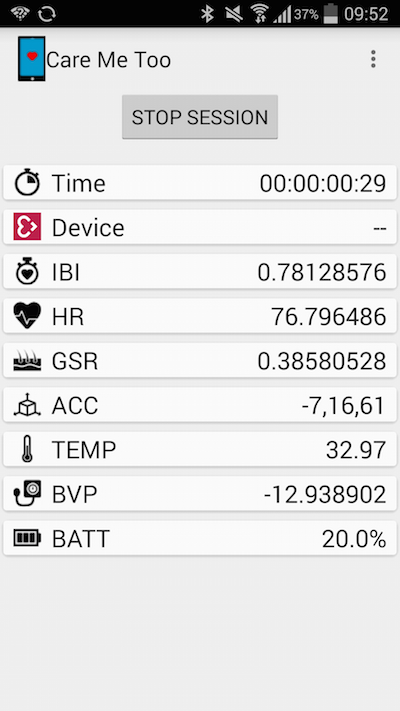
\includegraphics[height=80mm]{./Figures/img_caremetoo}}
        \caption{La aplicaci\'on Care Me Too mostrando se\~nales fisiol\'ogicas siendo grabadas.}\label{fig:caremetoo}
\end{figure}

Para obtener datos del ritmo card\'iaco de la banda Zephyr HxM se utiliz\'o el programa de l\'inea de comandos ``anxiLogger''\footnote{https://github.com/panzerfausten/anxiLogger} desarrollado por el autor para un estudio anterior \citep{Miranda}. El archivo csv de salida fue agregado a los datos de sesi\'on para sincronizar los tiempos a trav\'es de una librer\'ia llamada ``maxiProcesser''\footnote{https://github.com/panzerfausten/maxiProcesser}
	Para la banda Muse se us\'o la aplicaci\'on de escritorio ``Muse lab''. Los datos obtenidos en formato .muse fueron exportados a .csv para analizarlos posteriormente.

	Se us\'o una laptop Macbook en el sitio para conectar las bandas Muse y Zephyr y un tel\'efono inteligente Samsung Galaxy S4 para colectar datos. Los datos del participante observador fueron obtenidos a trav\'es de una segunda pulsera Empatica E3 en modo de grabaci\'on. Este modo no requiere de una conexi\'on bluetooth.


\section{Obtenci\'on de l\'inea base}\label{secc:dataanalysis}
Un reto del estudio de usuario fue identificar cuando los participantes sent\'ian ansiedad. Para lograrlo, se utilizaron tres diferentes t\'ecnicas: An\'alisis de video, observaci\'on directa y autoreportado. La figura ~\ref{fig:labeling} muestra el proceso unificado de etiquetado. A continuaci\'on se explica el procesamiento de cada fuente.

\begin{figure}[h]
        \centering
        \subfigure[]{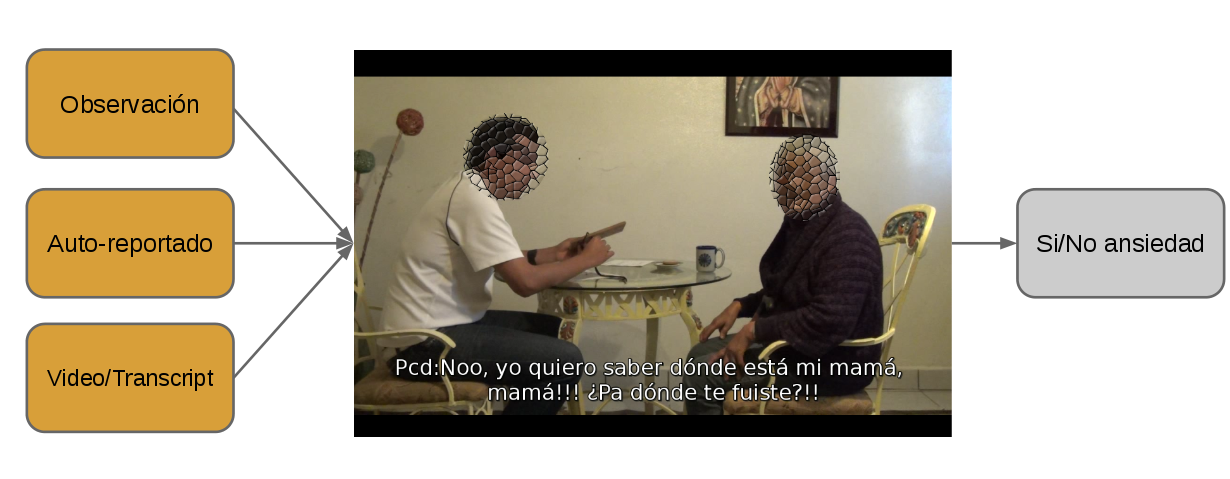
\includegraphics[height=100mm,width=160mm,keepaspectratio]{./Figures/img_labeling}}
	\caption{Proceso de etiquetado a partir de tres diferentes fuentes.}\label{fig:labeling}
\end{figure}
	\subsection{Procesamiento de video}\label{secc:videoprocesing}

	Todos los videos fueron transcritos utilizando el programa F5 transkript para Mac OS X. Con el archivo de transcripci\'on, se generaron subt\'itulos para facilitar el an\'alisis. Luego, se etiquet\'o linea por linea el comportamiento del actor de un adulto mayor con demencia. Cada linea fue clasificada en una de los tres posibles niveles que cumplieran con un criterio (ver tabla ~\ref{table:anxilevels}).  La figura ~\ref{fig:f5transcript} muestra una porci\'on de la transcripci\'on de la sesi\'on de un participante
\begin{figure}[h!]
        \centering
        \subfigure[]{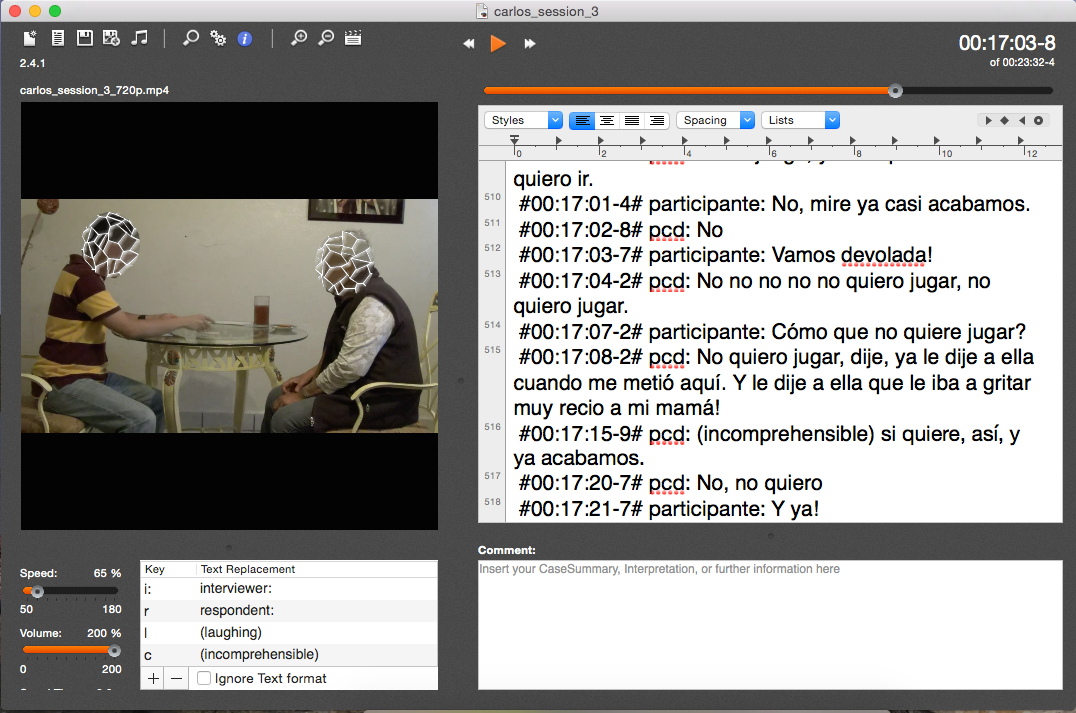
\includegraphics[height=10cm,keepaspectratio]{./Figures/img_experiment.png}}
        \caption{Transcripci\'on correspondiente a una sesi\'on completa de un participante}\label{fig:f5transcript}
\end{figure}

%La figura ~\ref{fig:imgsegment} ejemplifica un segmento extra\'ido. En el siguiente cap\'itulo se explica como se clasificaron los datos y los resultados de la detecci\'on.

%\begin{figure}[h]
%        \centering
%        \subfigure[]{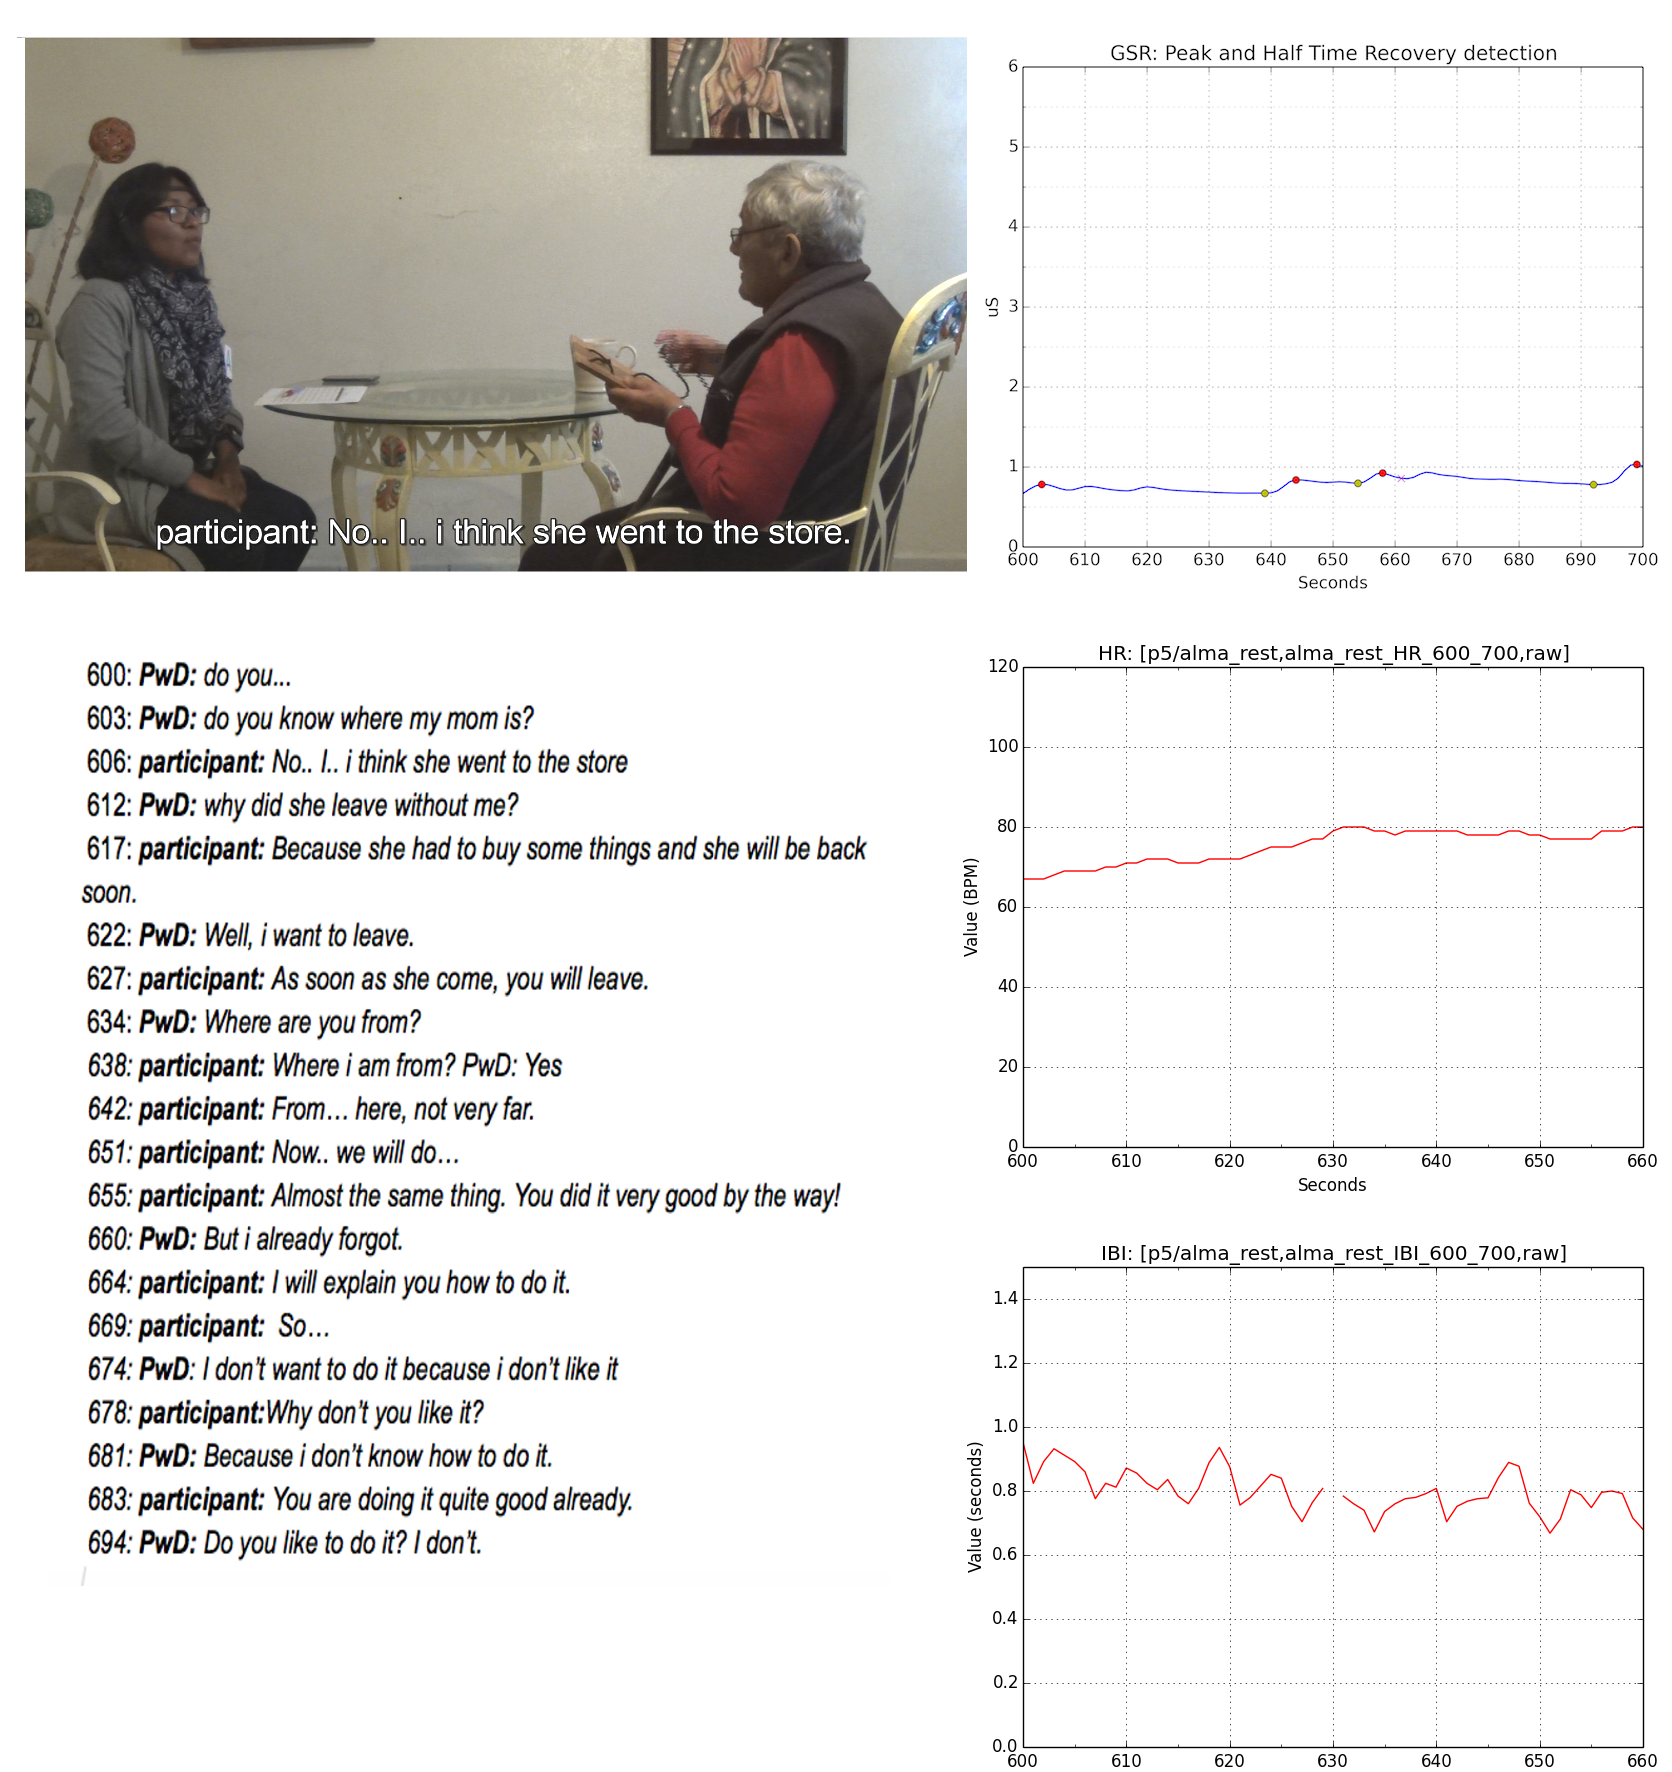
\includegraphics[height=18cm,keepaspectratio]{./Figures/img_segment.png}}
%        \caption{Transcripci\'on y se\~nales GSR, HR, e IBI correspondientes a una situaci\'on estresante}\label{fig:imgsegment}
%\end{figure}

	\subsection{Observaci\'on}
	Dos investigadores realizaron observaci\'on en el sitio, tomando nota del tiempo, nivel del comportamiento del actor de un adulto mayor con demencia, y una descripci\'on del evento. Esta descripci\'on fue escrita en base a lo que el participante y/o la aPcD dijo o hizo en el momento. El nivel de comportamiento fue codificado en base a la tabla ~\ref{table:anxilevels}. Esta codif\'ificaci\'on no es un instrumento de medici\'on de ansiedad, sino una clasificaci\'on que describe el comportamiento del aPcD y ayuda como informaci\'on extra para pasos posteriores. La secci\'on ~\ref{secc:unificacion} muestra como esta informaci\'on es unida con otras fuentes. Un evento etiquetado como ``0'' corresponde a cuando la aPcD se encuentra realizando la tarea como se le pidi\'o. En esta situaci\'on el cuidador puede estar totalmente relajado o bien ligeramente estresado. En un evento con la etiqueta ``1'' la aPcD se encuentra en un estado renuente diciendo cosas como ``No me gusta esta tarea'' o ``Hazlo tu, yo no quiero''. La aPcD podr\'ia estar realizando la tarea con bajo rendimiento o podr\'ia no prestar atenci\'on del todo. En un nivel ``2'', la aPcD realiza situaciones no esperadas como preguntar al participante por su madre o cualquier otra pregunta que lo ponga inc\'omodo. La atenci\'on hacia la tarea puede ser muy baja. En el nivel ``3'', la aPcD realiza acciones como tratar de golpear al participante, levantarse de la silla y querer salir de la habitaci\'on o gritar. La atenci\'on a la tarea suele ser nula. La figura~\ref{fig:imgobservation} ejemplifica la observaci\'on correspondiente a una sesi\'on.

	\begin{table}[h!]
		\footnotesize
		\centering
		\caption{Criterio de etiquetado de comportamiento de la aPcD.}
		\label{table:anxilevels}
		%\rotatebox{90}{
		\begin{tabular}{m{2.5cm}m{5.0cm}m{5.0cm}m{2.5cm}}
			\hline\noalign{\smallskip}

		    \textbf{Nivel} & \textbf{Criterio}                                                                                    & \textbf{Ejemplo de evento}                                                                      \\ \hline
			\\ \noalign{\smallskip}

			    0     & \pbox{12cm}{La aPcD actua de forma pasiva,\\La aPcD accede a participar,  \\El participante y la aPcD \\est\'an haciendo la tarea} &                   \pbox{12cm}{La aPcD est\'a realizando la\\ tarea como se le pidi\'o.}                       \\ 
	      1     & \pbox{12cm}{Comportamientos renuentes.,\\Reacio a participar,\\Quejandose acerca de la tarea.}                & \pbox{12cm}{ ``No me gusta este juego.'' \\ ``Esto es muy dif\'icil.'' \\``Hazlo tu.'' }             \\ 
	      2     & \pbox{12cm}{Murmureo,\\Hablando cosas sin sentido,  \\Comportamientos impredecibles}                                      & \pbox{5cm}{``?`Donde est\'a mi mam\'a?''\\``Qui\'en eres?''}                                          \\ 
	      3     & \pbox{12cm}{Gritos.\\Amenazas al particpante,\\Paranoia,  \\Urgencia de irse.}                          & \pbox{12cm}{``MAM\'A, DONDE EST\'AS!!??''\\``YA QUIERO IRME!''  \\``QUIEN ERES? D\'EJAME IR!'' } \\ 
		\end{tabular}
		%}
	\end{table}
\begin{figure}[h]
        \centering
        \subfigure[]{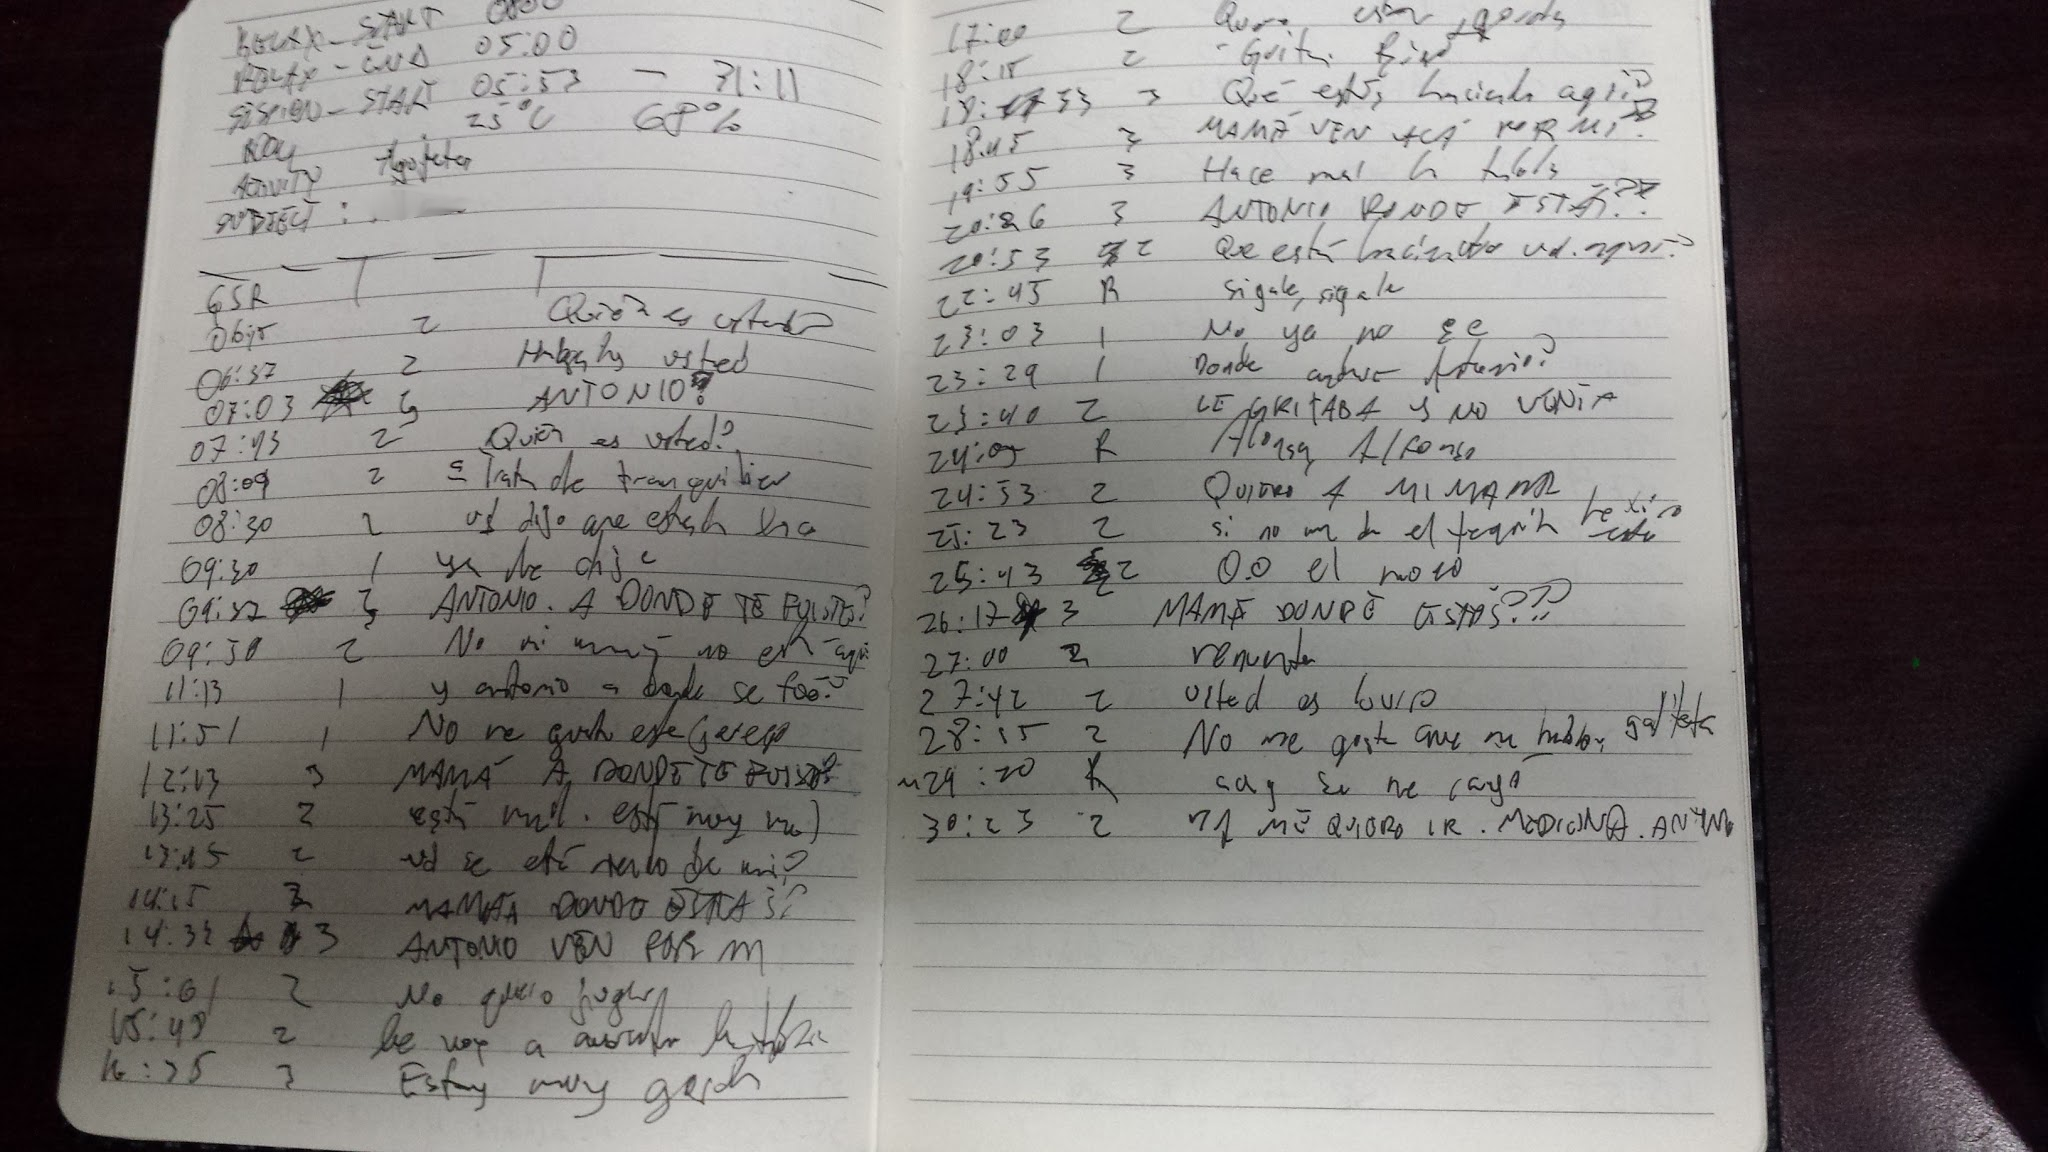
\includegraphics[height=200mm,width=160mm,keepaspectratio]{./Figures/img_observation.png}}
        \caption{Libreta de observaci\'on. Se anot\'o el tiempo con respecto al inicio de la sesi\'on, el nivel de evento de la aPcD percibido y una porci\'on del dialogo como referencia. Otros datos como la temperatura y humedad relativa del cuarto fueron anotados.}\label{fig:imgobservation}
\end{figure}
	\subsection{Autoreportado}
	Se les entreg\'o a los participantes un formulario en papel para indicar su nivel de ansiedad mientras desarrollaban la tarea. La escala del nivel de ansiedad fue tomada de la escala de ansiedad subjetiva autocalificada explicada en el ~\ref{capit:cap2}. Se les explic\'o a los participantes durante la sesi\'on de entrenamiento como utilizar el formulario de auto reportado. Sin embargo, algunos de ellos encontraron dif\'icil de contestarlo adecuadamente, principalmente porque estaban muy ocupados con la terapia. La figura ~\ref{fig:imggtlabel} ejemplifica el auto reportado de un participante que contest\'o correctamente el formulario.
	\begin{figure}[h!]
		\centering
		\subfigure[]{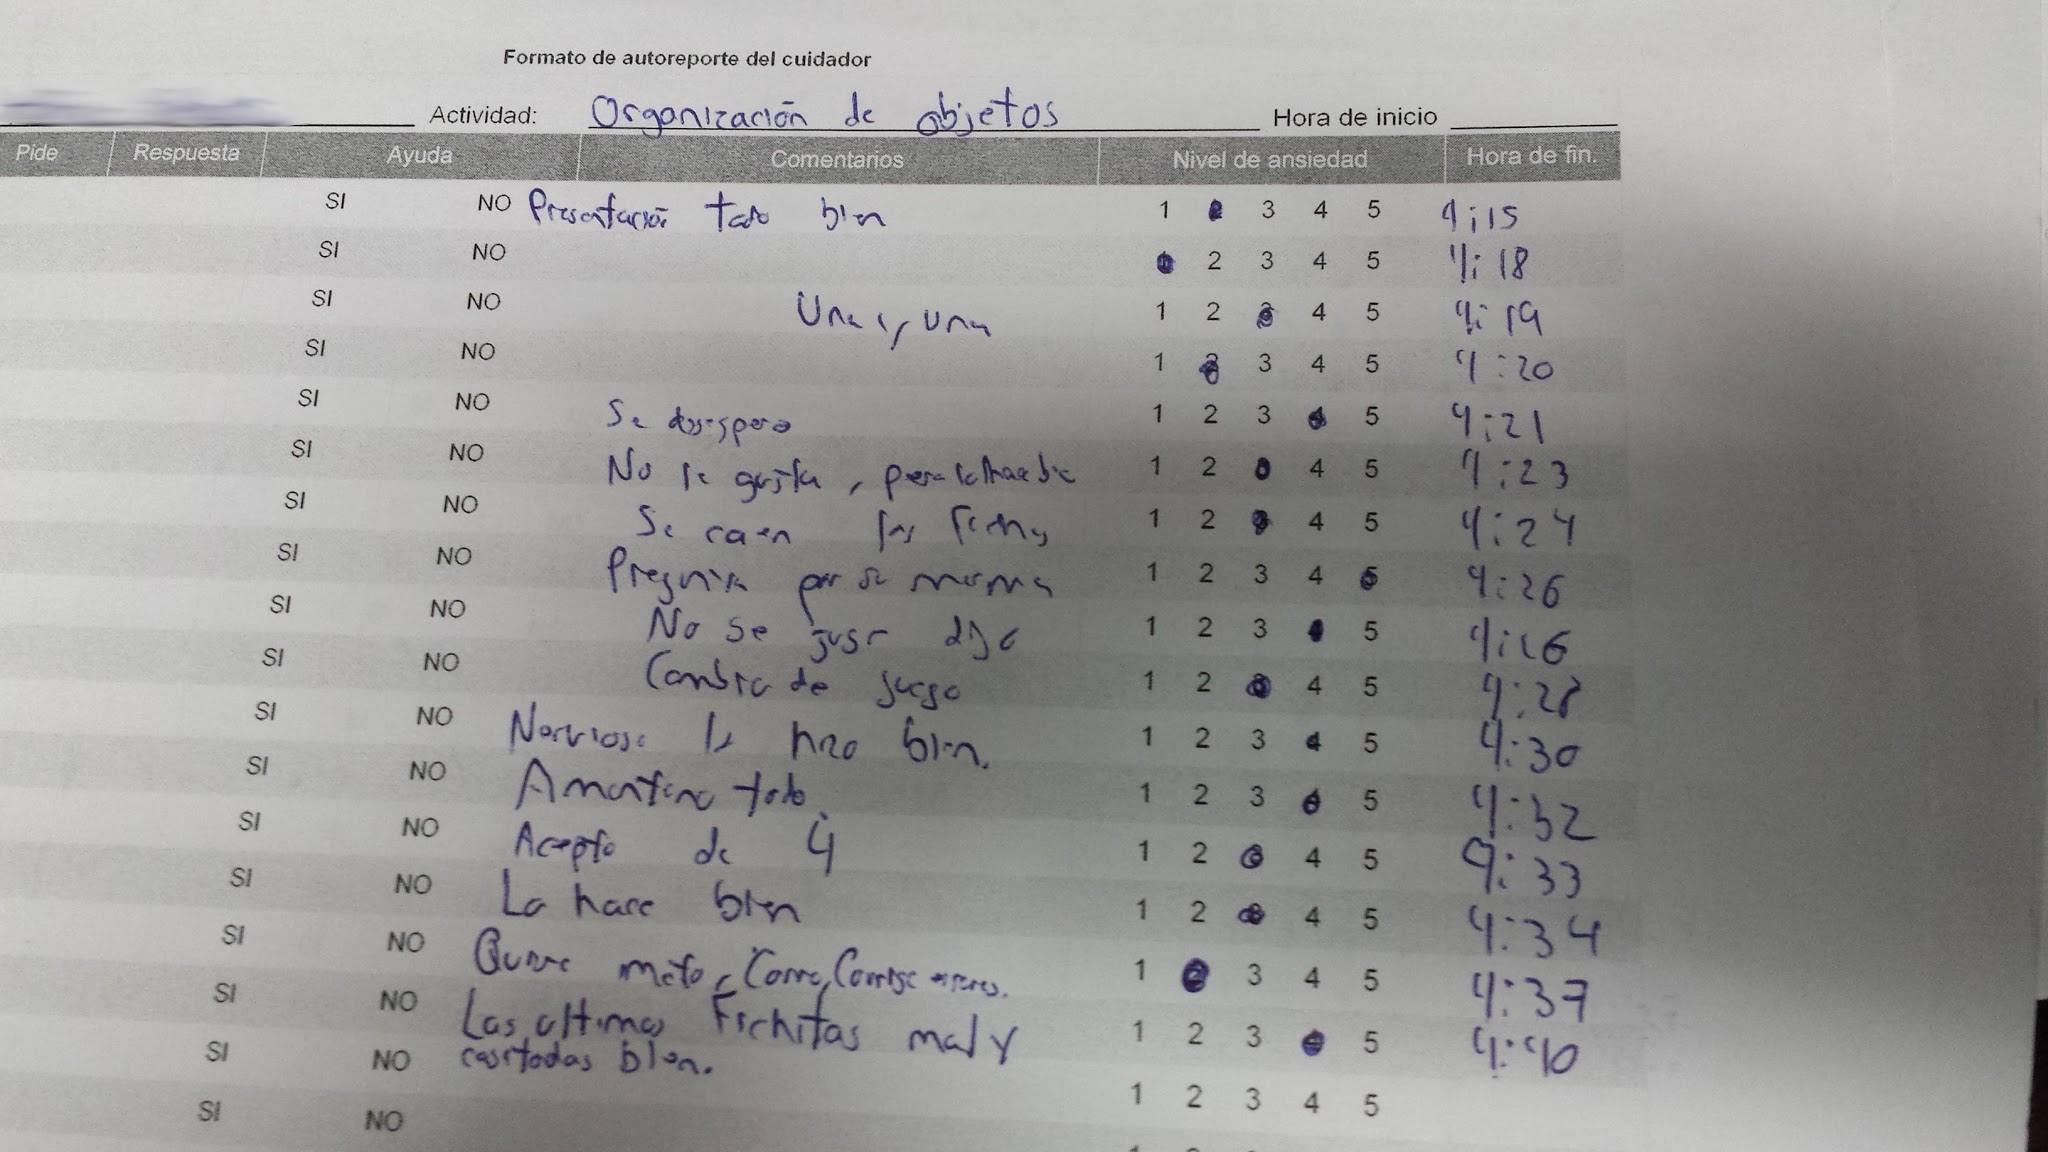
\includegraphics[height=200mm,width=160mm,keepaspectratio]{./Figures/img_sr.png}}
		\caption{Formato de auto reportado de una sesi\'on completa de un participante}\label{fig:imggtlabel}
	\end{figure}

	\subsection{Unificaci\'on de l\'inea base}\label{secc:unificacion}
	Por \'ultimo, se gener\'o un formato con los datos de transcripci\'on, nivel del evento del actor de un adulto mayor con demencia y auto reportado. Al mismo tiempo, se observ\'o el video para obtener rasgos de ansiedad como cambios en la tonalidad de voz, desv\'io de mirada, o movimientos del participante. Con esta informaci\'on, se etiquet\'o cada 30 segundos si exist\'ia ansiedad o no. Se anot\'o con el n\'umero ``1'' cuando claramente el participante experimentaba ansiedad y con un ``0'' si claramente no. Si el segmento era muy ambiguo (p. ej. El participante se ve ansioso en el video pero el nivel del auto reportado y el evento de la PcD eran bajos) se etiquet\'o con el n\'umero ``-1''. La figura ~\ref{fig:imggtlabel} ejemplifica un segmento codificado.
	\begin{figure}[h!]
		\centering
		\subfigure[]{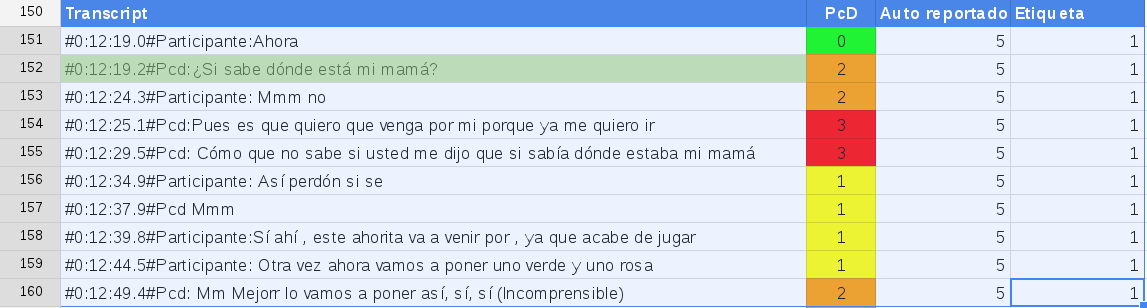
\includegraphics[height=200mm,width=160mm,keepaspectratio]{./Figures/img_gtlabel.png}}
		\caption{Segmento codificado como ansiedad. El nivel de auto reportado es alto y existen valores altos en el comportamiento de la aPcD. }\label{fig:imggtlabel}
	\end{figure}
\section{Preprocesamiento de GSR}\label{secc:gsrpreprocessing}
Se desarroll\'o una librer\'ia en python para procesar todos los datos fisiol\'ogicos, incluyendo funciones para exportar, extraer caracter\'isticas, sincronizaci\'on de tiempos, y graficado de datos de ansiedad de todos los dispositivos. La librer\'ia tambi\'en puede graficar atributos de la se\~nal GSR (picos, tiempos de recuperaci\'on medios, amplitudes, etc.) y guardar los datos en formato .csv y .json.

Se inici\'o remuestreando los datos de GSR de 4.0 Hz a 1.0 Hz calculando el valor promedio de todos los datos que cayeran en una ventana deslizante de 1 segundo. Esto se hizo debido a que se esperaba que los periodos de ansiedad duraran segundos. Luego, se aplic\'o un filtro gausiano para suavizar la se\~nal y el ruido. Finalmente, se us\'o un m\'etodo de la librer\'ia scipy de python para detectar picos y se filtraron todos los picos con amplitud mas grande que un umbral ($t \geqslant 0.04$ para datos no normalizados y $t \geqslant 0.01$ para datos normalizados en base a experimentaci\'on e inspecci\'on visual) con la finalidad de evitar variaciones dadas por el sensor o muy peque\~nas para tener una utilidad. Tambi\'en se calcul\'o el ``Tiempo de media recuperaci\'on'' de la se\~nal. Esto es, el punto donde la se\~nal decae al valor exacto de la mitad del pico.
\section{Preprocesamiento de HR e IBI}\label{secc:hribipreprocessing}
No fue necesario remuestrear los datos de HR e IBI debido a la naturaleza de la se\~nal. El sensor solo reporta datos cuando ocurre un latido del coraz\'on. Sin embargo, se agrup\'o en ventanas de segundos para compararlo con el resto de las se\~nales. El ruido de los datos fu\'e muy bajo y no requiri\'o pre-procesamiento adicional.
\section{Extracci\'on de caracter\'isticas}
Una vez segmentadas y etiquetadas las sesiones, se tomaron varias caracter\'isticas por cada tipo de se\~nal. Estas caracter\'isticas generalizan al evento completo. La tabla ~\ref{tab:features} describe dichas caracter\'isticas.

	\begin{table}[t]
		\footnotesize
		\centering
        	\caption{Caracter\'isticas usadas como entrada para el clasificador de SVM}
 	       \label{tab:features}

		%\rotatebox{90}{
		\begin{tabular}{m{2.5cm}m{5.0cm}m{5.0cm}m{2.5cm}}
			\hline\noalign{\smallskip}

                \textbf{Se\~nal} & \textbf{Caracter\'istica} & \textbf{Descripci\'on} & \textbf{Unidad} \\
		\hline
			\\ \noalign{\smallskip}
                GSR   & \pbox{12cm}{\textit{Amplitud de los picos}}                & \pbox{12cm}{Distancias promedio \\desde el punto de crecimiento\\ hacia el pico}             & \pbox{12cm}{$\mu S$}        \\
                GSR   & \pbox{12cm}{\textit{Amplitud m\'axima de los picos}}                & \pbox{12cm}{Amplitud mas grande \\ de los picos}             & \pbox{12cm}{$\mu S$}        \\
                GSR   & \pbox{12cm}{\textit{Amplitud m\'inima de los picos}}                & \pbox{12cm}{Amplitud mas chica \\ de los picos}             & \pbox{12cm}{$\mu S$}        \\
                GSR   & \pbox{12cm}{\textit{Varianza de los picos}}                & \pbox{12cm}{Varianza total de todos\\ los picos}             & \pbox{12cm}{$\mu S$}        \\
			GSR   & \pbox{12cm}{\textit{Tiempo promedio de} \\\textit{media recuperaci\'on de los picos}}                & \pbox{12cm}{Varianza total de todos\\ los picos}             & \pbox{12cm}{$\mu S$}        \\
                IBI   &\textit{M\'inimo}                & Valor m\'inimo del segmento            &Segundos       \\
                IBI   &\textit{M\'aximo}                & Valor m\'aximo del segmento            &Segundos       \\
                IBI   &\textit{Promedio}                & Valor promedio del segmento            &Segundos       \\
                IBI   &\textit{Desviaci\'on estandar}                &  \pbox{12cm}{Desviaci\'on estandar de todos\\ los datos del segmento}            &Segundos        \\


        \end{tabular}
\end{table}
%TODO:UPDATE THIS 
%Para este trabajo, se tuvo un total de 51 segmentos del nivel 0, 177 del nivel 1, 145 del nivel 2 y 106 del nivel 3. Los datos corresponden a 5 del total de 10 de participantes. Utilizando 15 sesiones. No se procesaron todas las sesiones en su totalidad, debido al extenso tiempo necesario para transcribir los videos. Todos los segmentos fueron luego codificados en forma de vectores descriptores. Estos vectores fueron guardados en formato .csv, con la primera columna correspondiente a la etiqueta de nivel de ansiedad.
%\section{Sincronizaci\'on de datos}
%	Agregar 
\section{Conclusi\'on}
El dise\~no de este estudio de usuario permite capturar datos de actores en un escenario concreto de cuidadores de personas con demencia que simulan condiciones cercanas a las reales. Esto abre la posibilidad de analizar por medio de tecnolog\'ia los efectos de ansiedad en los cuidadores.

En la siguiente secci\'on se utiliza una t\'ecnica de aprendizaje de m\'aquina para clasificar los eventos de ansiedad. Se explican las diferentes pruebas realizadas, y los resultados generales de este estudio de usuario.
\newpage
%%=====================================================


%EndExpansion
\newpage }

{\normalsize
%TCIMACRO{\QSubDoc{Include Capitulo04}{
\chapter{Very título}\label{capit:cap4}
\vspace{-2.0325ex}%
\noindent
\rule{\textwidth}{0.5pt}
\vspace{-5.5ex}% 
\newcommand{\pushline}{\Indp}% Indent puede ir o no :p

Sobre referencias. CICESE pide este formato \citep{Adleman1998}


\newpage
%%=====================================================
} }%
%BeginExpansion

\chapter{Very título}\label{capit:cap4}
\vspace{-2.0325ex}%
\noindent
\rule{\textwidth}{0.5pt}
\vspace{-5.5ex}% 
\newcommand{\pushline}{\Indp}% Indent puede ir o no :p

Sobre referencias. CICESE pide este formato \citep{Adleman1998}


\newpage
%%=====================================================

%EndExpansion
\newpage }

{\normalsize
%TCIMACRO{\QSubDoc{Include Capitulo05}{
\chapter{Conclusiones y trabajo a futuro}\label{capit:cap5}
\vspace{-2.0325ex}%
\noindent
\rule{\textwidth}{0.5pt}
\vspace{-5.5ex}% 
\newcommand{\pushline}{\Indp}% Indent puede ir o no :p


\newpage
%%=====================================================
} }%
%BeginExpansion

\chapter{Conclusiones y trabajo a futuro}\label{capit:cap5}
\vspace{-2.0325ex}%
\noindent
\rule{\textwidth}{0.5pt}
\vspace{-5.5ex}% 
\newcommand{\pushline}{\Indp}% Indent puede ir o no :p


\newpage
%%=====================================================

%EndExpansion
\newpage }


\linespread{1.0}
\addcontentsline{toc}{chapter}{\normalsize\expandafter{Lista de referencias}}
{\normalsize
\bibliographystyle{cicese}%cicese, ieeetr, plain, unsrt, alpha, abbrv, acm, apalike 
\nocite{*}
\bibliography{iTesis}
}

\linespread{1.5}
{\normalsize
%TCIMACRO{\QSubDoc{Include Apendice}{\appendix{}

\chapter{Instrumentos y protocolos de diagnóstico} \label{aped:A_instrumentos}
\vspace{-3ex}%
\noindent
\rule{\textwidth}{1pt}
\vspace{-2ex}%

Lorem ipsum dolor sit amet, consectetur adipiscing elit. Aliquam sit amet lobortis turpis. Praesent auctor mi metus, sed bibendum ligula efficitur eu. Suspendisse ut ante id erat interdum accumsan. Pellentesque eget hendrerit eros, et ullamcorper elit. Proin a lacus et sem hendrerit efficitur. Praesent eget eros sed tellus dapibus bibendum sit amet vel justo. Maecenas finibus porttitor dictum. Fusce lacinia dictum interdum.

Proin aliquam laoreet luctus. Vivamus ipsum nulla, dapibus nec turpis consequat, imperdiet dictum ipsum. Nunc augue purus, accumsan sed venenatis eget, lacinia id lorem. Praesent et sapien in velit dapibus congue. Curabitur vitae velit nisi. Nam tellus elit, tincidunt blandit mauris ut, porttitor eleifend sem. Nunc sed varius orci. Nunc varius consectetur felis quis ultricies. Duis accumsan diam nulla, egestas porttitor nisi fringilla et. Duis ut leo odio. Vestibulum ante ipsum primis in faucibus orci luctus et ultrices posuere cubilia Curae; Pellentesque malesuada dui quis nisi sollicitudin venenatis. Nulla facilisi.

Nunc hendrerit justo vitae leo imperdiet, eu egestas nunc tristique. Etiam eget risus purus. Suspendisse sagittis tellus eu ipsum ultrices porttitor. Aliquam iaculis, metus sed ullamcorper blandit, justo nibh vehicula ipsum, vitae finibus diam orci vitae magna. Donec sit amet orci a dui laoreet euismod. Sed sed justo eget metus fermentum lacinia quis eget tellus. Pellentesque nibh metus, auctor id felis sed, lobortis condimentum urna. Nullam vel pharetra nisi. Sed volutpat nisi at efficitur blandit. Nulla interdum dictum dui, nec laoreet diam vulputate non. Lorem ipsum dolor sit amet, consectetur adipiscing elit. Suspendisse non lobortis elit, vel bibendum tellus. Praesent gravida feugiat metus, non ultricies nunc mattis ut. Sed eget interdum velit.

Mauris et imperdiet tortor. Maecenas consectetur lacus elit, dignissim eleifend dolor ornare ut. Aenean euismod porta nisi, et volutpat ex laoreet sit amet. Sed ac elit vestibulum neque ultrices feugiat. Class aptent taciti sociosqu ad litora torquent per conubia nostra, per inceptos himenaeos. Aenean tincidunt, enim eget finibus accumsan, orci nisl condimentum odio, at condimentum elit nisi at mauris. Nam sapien justo, tempor id ornare in, rutrum sit amet nisi. Sed arcu magna, egestas a sollicitudin eleifend, blandit et ex. Vestibulum sed euismod sem. Sed non quam lobortis mauris interdum tincidunt. Integer luctus tortor sed risus sagittis pretium. Vivamus pellentesque justo eu tincidunt accumsan. Suspendisse sed erat in metus maximus ornare vel quis turpis. Morbi pharetra orci sem, vel pretium leo dictum in.

Aenean id nisl dapibus, hendrerit massa nec, mattis tortor. Maecenas tempus risus risus, eu lacinia libero vestibulum volutpat. Phasellus ac mi ligula. Cum sociis natoque penatibus et magnis dis parturient montes, nascetur ridiculus mus. Aliquam rutrum rhoncus auctor. Phasellus sit amet ligula ut enim tristique vestibulum at dictum nisi. Nunc suscipit laoreet tellus tempus placerat. Proin porta, orci vel ornare faucibus, augue justo euismod nisl, non semper turpis sem quis mauris. Praesent ut interdum sem. Vestibulum eu malesuada nunc. Curabitur suscipit ligula libero, at pellentesque lacus iaculis sed. Proin porta dolor volutpat dui tempor commodo. Donec id est hendrerit, bibendum nisl ut, tempus nibh. Nullam vitae tincidunt velit.



\begin{table}
\centering
\caption{Praesent eget eros sed tellus dapibus bibendum sit amet vel justo. Maecenas finibus porttitor dictum. Fusce lacinia dictum interdum.}
\label{tab:unidimencional}
\rotatebox{90}{
\begin{tabular}{m{0.3cm}m{7cm}m{3.5cm}m{5.5cm}m{3cm}m{1.5cm}}
\hline\noalign{\smallskip}
& \textbf{CUESTIONARIO} & \textbf{POBLACIÓN} & \textbf{EVALUACIÓN} & \textbf{ESCALA} & \textbf{ÍTEMS}
\\ \noalign{\smallskip}
\hline
\noalign{\smallskip}
1	&	Brief Fatigue Inventory								&	Cancer							& 	Gravedad							&	Likert (11) 	& 	9 	 \\
2	&	Cancer-Related Fatigue Distress Scale				&	Cancer							& 	Impacto							& 	Likert (11) 	& 	20 	 \\ 
3	&	Daily Fatigue Impact Scale							&	MS, BI, PG						&	Impacto 							& 	Likert (5) 	& 	8 	 \\ 
4	&	Fatigue Severity Scale								&	MS, Pakirson, SDP, Cancer		&	Impacto y resutlados 			& 	Likert (7) 	& 	9 	 \\ 
5	&	Functional Assessment of Cancer Therapy				&	Cancer							&	Severidad e impacto 				& 	Likert (5) 	& 	13 	 \\ 
6	&	Global Vigour Affect									&	Cancer							&	Gravedad 						& 	Analogía visual 	& 	8 	 \\ 
7	&	May and Kline Adjective Checklist					&	Efectos de medicamentos, SDP		&	Fenomenología y severidad 		& 	Likert (9) 	&	16	 \\ 
8	&	Pearson–Byars Fatigue Feeling Checklist				&	No clínico						&	Severidad 						& 	Checklist	& 	26 	 \\ 
9	&	Rhoten Fatigue Scale									&	Cancer, embarazo					&	Severidad					 	& 	Likert (5) 	& 	1 	 \\ 
10	&	Screening for Prolonged Fatigue Syndrome (Prolonged Fatigue Syndrome and Chronic Fatigue Syndrome)
															&	Cancer, embarazo					&	Fenomenología y gravedad 		& 	Likert (5) 	& 	10 	 \\ 
11	&	Functional Assessment of Chronic Illness Therapy		&	Población geriátrica				&	Severidad e impacto	 			& 	Likert (4) 	& 	13 	 \\ 
\hline
\end{tabular}
}
\end{table}





\begin{table}
\small
\centering
\caption{Praesent eget eros sed tellus dapibus bibendum sit amet vel justo. Maecenas finibus porttitor dictum. Fusce lacinia dictum interdum.}
\label{tab:recopilacionDePruebasFisicas}
\rotatebox{90}{
\begin{tabular}{m{0.2cm}m{4cm}m{7cm}m{9cm}}
\hline\noalign{\smallskip}
& \textbf{NOMBRE} & \textbf{DESCRIPCIÓN} & \textbf{PARÁMETROS} 
\\ \noalign{\smallskip}
\hline
\noalign{\smallskip}
1	&	Test de Cooper	
		&	Prueba de resistencia que consiste en recorrer la mayor distancia posible en 12 minutos a una velocidad constante.							
		& 	Se mide el tiempo y la distancia recorrida para clasifica al participante de acuerdo a su nivel de condicionamiento físico: muy mala, mala, regular, buena, excelente.\\
2	&	Test de Conconi	
		&	El participante pedalea una bicicleta/corre con una carga cada vez más pesada hasta quedar exhausto.							
		& 	Se debe llevar un registro de la pulsación cardiaca, el tiempo, y el incremento de carga. Finalmente, los datos son sometidos a una relación pre-establecida a tavés de la cual se calcula el umbral anaeróbico.\\
3	&	Test de Course-Navette	
		&	El participante va desplazándose de un punto a otro situado a 20 metros de distancia, realizando cambio de sentido al ritmo indicado por una señal sonora que va acelerándose progresivamente.
		& 	Se debe registrar la edad, y velocidad máxima alcanzada para posteriormente evaluar la funcionalidad máxima de la potencia aeróbica que se identifica con el $VO_{2}$ Máx.\\
4	&	Yo-yo test
		&	El participante corre 20 metros y descansa 5. El ejercicio se realiza de manera consecutiva hasta completar 15 secuencias o quedar exhausto.					
		& 	Evalua la capacidad de trabajo de forma continua durante un periodo  de tiempo prolongado (resistencia). Al final los participantes son clasificados en: elite, excelente, bueno, promedio, abajo del promedio, y malo.\\
5	&	Test de Mognoni (6MWT)
		&	El participante recorre la distancia máxima posible durante 6 minutos.
		& 	Basta con llevar el registro de percepción de cansancio para determinar el esfuerzo realizado en la prueba, o bien la velocidad y distancia recorrida para evaluar el concentrado de lactato por litro de sangre del participante.\\	
6	&	Wingate Anaerobic cycle Test
		&	El participante pedalea de manera constante una bicicleta durante 10 minutos.
		& 	Llevando un registro de la distancia recorrida, tiempo, y peso del participante, es posible calcular: pico absoluto y relativo de la potencia de salida, fatiga y capacidad anaeróbica.\\
7	&	Margaria Kalamen Power Test
		&	Se mide el tiempo requerido de un sujeto para subir una serie de escalera la velocidad máxima. El tiempo se mide por dos pasos (de cuando un pie toca el segundo paso hasta que aterriza de nuevo).
		& 	Basta con llevar un control sobre la configuración del protocolo para calcular la potencia del participante.\\		
\hline
\end{tabular}
}
\end{table}

\pagebreak
\subsection{Carta de consentimiento informativo de participantes en el proyecto de investigación}\label{aped:A_cartaConsentiemiento}
Lorem ipsum dolor sit amet, consectetur adipiscing elit. Aliquam sit amet lobortis turpis. Praesent auctor mi metus, sed bibendum ligula efficitur eu. Suspendisse ut ante id erat interdum accumsan. Pellentesque eget hendrerit eros, et ullamcorper elit. Proin a lacus et sem hendrerit efficitur. Praesent eget eros sed tellus dapibus bibendum sit amet vel justo. Maecenas finibus porttitor dictum. Fusce lacinia dictum interdum.

Proin aliquam laoreet luctus. Vivamus ipsum nulla, dapibus nec turpis consequat, imperdiet dictum ipsum. Nunc augue purus, accumsan sed venenatis eget, lacinia id lorem. Praesent et sapien in velit dapibus congue. Curabitur vitae velit nisi. Nam tellus elit, tincidunt blandit mauris ut, porttitor eleifend sem. Nunc sed varius orci. Nunc varius consectetur felis quis ultricies. Duis accumsan diam nulla, egestas porttitor nisi fringilla et. Duis ut leo odio. Vestibulum ante ipsum primis in faucibus orci luctus et ultrices posuere cubilia Curae; Pellentesque malesuada dui quis nisi sollicitudin venenatis. Nulla facilisi. 


} }%
%BeginExpansion
\appendix{}
\chapter{intrumentos para el dise\~no del experimento}\label{aped:A}
\subsection{Carta de consentimiento informado de participantes en el proyecto de investigaci\'on} \label{aped:cartainfo}
\vspace{-3ex}%
\noindent
\rule{\textwidth}{1pt}
\vspace{-2ex}%

Por medio de la presente acepto participar en el proyecto de investigación que CICESE realiza, titulado: \textbf{``Monitoreo por sensores electrónicos en adultos mayores sanos en Ensenada, B.C,''}, a llevarse a cabo en esta ciudad de Mayo a Septiembre de 2015.

\textbf{El objetivo de este estudio es:} Obtener información capturada a través de teléfonos celulares  inteligentes, de las actividades cotidianas que realizan los adultos mayores de 65 años de edad.

\textbf{Se me ha explicado que mi participación consistirá en:}  Llevar a cabo sesiones de terapias a adultos mayores con Alzheimer de alrededor de una hora de duración. También se me informó que debo de contestar a diversas preguntas sobre mi desempeño en la terapia en forma de cuestionarios. Por último, fui informado que recibiré una compensación de un pase doble al cine en la pelicula disponible de mi elección al termino de la sesión.

\textbf{Se me ha informado ampliamente sobre los posibles riesgos, inconvenientes, molestias y beneficios derivados de la participación en el estudio.}

Podré dejar de contestar cualquier pregunta  si no es mi deseo, o si dudo de la respuesta.
El investigador principal se ha comprometido a responder cualquier pregunta y aclarar cualquier duda que tenga, acerca de los procedimientos que se llevarán a cabo, o cualquier otro asunto relacionado con la investigación.
Entiendo que conservo el derecho a retirarme del estudio en cualquier momento en que lo considere conveniente.
Los investigadores a cargo del proyecto me ha asegurado de que no se me identificará en las presentaciones o publicaciones que se deriven de este estudio, y que los datos recabados  serán manejados en manera confidencial. Al mismo tiempo se me ha asegurado, que si así lo deseo, se me proporcionará la información que se derive del estudio.

Nombre, firma y domicilio del participante
\pagebreak
\subsection{Carta de no divulgaci\'on de participantes en el proyecto de investigaci\'on} \label{aped:cartanodiv}
\vspace{-3ex}%
\noindent
\rule{\textwidth}{1pt}
\vspace{-2ex}%

El siguiente documento describe la manera en que los participantes deberán de hacer uso de la información generada durante las actividades del estudio con el fin de asegurar la calidad de los datos obtenidos.

Definiciones:
\begin{itemize}
        \item \textbf{Participante:} Persona reclutada para realizar las actividades durante el estudio.
        \item \textbf{Adulto Mayor:} Persona reclutada con la cual el participante realizará las actividades durante el estudio.
        \item \textbf{Investigadores:} Personal del CICESE (estudiante de posgrado, profesor o auxiliar de investigador) responsable del estudio.
\end{itemize}
Dentro de las limitaciones, el participante no podrá:
\begin{itemize}
        \item Comentar la situación mental o física del adulto mayor.
        \item Describir las actividades que realizó durante las terapias.
        \item Compartir técnicas o cualquier otra información que pueda ser utilizada para afectar el resultado de las terapias de otros participantes.
\end{itemize}

Todas las inquietudes o dudas deben de ser canalizadas a través de los investigadores por las formas de contacto proporcionadas.

Todas estas limitaciones son vigentes durante el tiempo de la intervención. Una vez que todos los participantes hayan terminado su participación este acuerdo será invalidado.

Nombre, firma y domicilio del participante

\appendix{}

\chapter{Carta de no divulgaci\'on de participantes en el proyecto de investigaci\'on} \label{aped:B}
\vspace{-3ex}%
\noindent
\rule{\textwidth}{1pt}
\vspace{-2ex}%

El siguiente documento describe la manera en que los participantes deberán de hacer uso de la información generada durante las actividades del estudio con el fin de asegurar la calidad de los datos obtenidos.

Definiciones:
\begin{itemize}
	\item \textbf{Participante:} Persona reclutada para realizar las actividades durante el estudio.
	\item \textbf{Adulto Mayor:} Persona reclutada con la cual el participante realizará las actividades durante el estudio.
	\item \textbf{Investigadores:} Personal del CICESE (estudiante de posgrado, profesor o auxiliar de investigador) responsable del estudio.
\end{itemize}
Dentro de las limitaciones, el participante no podrá:
\begin{itemize}
	\item Comentar la situación mental o física del adulto mayor. 
	\item Describir las actividades que realizó durante las terapias. 
	\item Compartir técnicas o cualquier otra información que pueda ser utilizada para afectar el resultado de las terapias de otros participantes.
\end{itemize}

Todas las inquietudes o dudas deben de ser canalizadas a través de los investigadores por las formas de contacto proporcionadas.

Todas estas limitaciones son vigentes durante el tiempo de la intervención. Una vez que todos los participantes hayan terminado su participación este acuerdo será invalidado.

Nombre y firma del participante

Domicilio del participante

%EndExpansion
\newpage }



\end{document}
